\documentclass{article}

%\usepackage{corl_2023} % Use this for the initial submission.
%\usepackage[final]{corl_2023} % Uncomment for the camera-ready ``final'' version.
\usepackage[preprint]{corl_2023} % Uncomment for pre-prints (e.g., arxiv); This is like ``final'', but will remove the CORL footnote.

% ### custom packages start ###
% math
\usepackage{amsmath,amsfonts,amssymb,amsthm}
\usepackage{mathtools}
\usepackage{commath}
\DeclareMathOperator*{\argmax}{arg\,max}
\DeclareMathOperator*{\argmin}{arg\,min}

% tables
\usepackage{array}
\usepackage{booktabs}
\usepackage{multirow}

% figures
\usepackage{subcaption}
\usepackage{wrapfig}

% algorithms
\usepackage{algorithm}
\usepackage{algpseudocode}
\newcommand{\minuseq}{\mathrel{-}=}

% colors
\usepackage{color}  % CoRL uses color insted of xcolor.
\definecolor{purple}{rgb}{0.5,0.0,0.5}
\definecolor{olive}{rgb}{0.5,0.5,0.0}
\newcommand{\ob}[1]{\textcolor{purple}{[\textbf{OB:} #1]}}
\newcommand{\evdp}[1]{\textcolor{blue}{[\textbf{EvdP:} #1]}}
\newcommand{\lsw}[1]{\textcolor{olive}{[\textbf{lsw:} #1]}}
\newcommand{\rob}[1]{\textcolor{green}{[\textbf{rob:} #1]}}
\newcommand{\tk}[1]{\textcolor{magenta}{[\textbf{TK:} #1]}}
\newcommand{\rst}
[1]{\textcolor{red}
{[\textbf{ST:} #1]}}


% highlight
\usepackage{soul}
\definecolor{lightlightgrey}{rgb}{0.9,0.9,0.9}
\sethlcolor{lightlightgrey}

% notation
\newcommand{\pcx}[1]{\mathrm{pcd}^{(#1)}}
\newcommand{\wxy}[2]{W_{#1 \rightarrow #2}}
\newcommand{\pci}{\pcx{i}}
\newcommand{\pcj}{\pcx{j}}
\newcommand{\pcc}{\pcx{C}}
\newcommand{\wij}{\wxy{i}{j}}
\newcommand{\wci}{\wxy{C}{i}}

% ### custom packages end ###

% \title{SA-Warp: Simple $\mathrm{SE}(3)$ Object Re-arrangement \\via Shape and Action Warping}

% \title{Simple $\mathrm{SE}(3)$ Object Re-arrangement \\via Shape and Action Warping}

% didn't like the title above, but not sure how I feel about this one either...

% \title{One-Shot Imitation Learning via Shape Warping}

\title{Imitation Learning via Simple Linear Shape Warping}

% \title{Keypoint Matching via Linear Shape Warping}

% The \author macro works with any number of authors. There are two
% commands used to separate the names and addresses of multiple
% authors: \And and \AND.
%
% Using \And between authors leaves it to LaTeX to determine where to
% break the lines. Using \AND forces a line break at that point. So,
% if LaTeX puts 3 of 4 authors names on the first line, and the last
% on the second line, try using \AND instead of \And before the third
% author name.

% NOTE: authors will be visible only in the camera-ready and preprint versions (i.e., when using the option 'final' or 'preprint'). 
% 	For the initial submission the authors will be anonymized.

\author{
  (Not final order) Ondrej Biza$^1$, Skye Thompson$^2$, Kishore Reddy Pagidi$^1$, Abhinav Kumar$^1$, \\
  \textbf{Elise van der Pol$^3$, Robin Walters$^1$, Thomas Kipf$^4$,} \\
  \textbf{Jan-Willem van de Meent$^{1,5}$, Lawson Wong$^1$, Robert Platt$^1$} \\
  $^1$ Northeastern University, $^2$ Brown University, $^3$ Microsoft Research, \\$^4$ Google Research, $^5$ University of Amsterdam \\
  \texttt{biza.o@northeastern.edu} \\
}


\begin{document}
\maketitle

%===============================================================================

\begin{abstract}
Imitation learning of robot policies from few demonstrations in crucial in open-ended applications. We propose a new method, Interaction Warping, for learning 3D robotic manipulation policies from a single demonstration. Our method infers the 3D mesh of each object in the environment using shape warping, a technique for aligning point clouds across object instances. We then use the warped meshes to transfer interaction points from a single demonstration to a scene with novel objects. The notion of interaction points allows us to transfer robot grasps and relational object placements. We show successful one-shot imitation learning on three simulated and real-world object re-arrangement tasks. We also demonstrate the ablity of our method to predict object meshes and robot grasps in the wild.
\end{abstract}

% Two or three meaningful keywords should be added here
\keywords{3D manipulation, imitation learning, shape warping.} 

%===============================================================================

% \begin{figure}[h]
%     \centering
%     \includegraphics[width=\textwidth]{figures/figure_9.pdf}
%     \caption{Examples of real-world generalization capabilities of SA-Warp. \ob{TODO: Reduce visual clutter, maybe masking or blurring.}}
%     \label{fig:intro}
% \end{figure}

\section{Introduction}


\begin{wrapfigure}[17]{r}{0.45\textwidth}
\vspace{-0.5cm}
  \begin{center}
    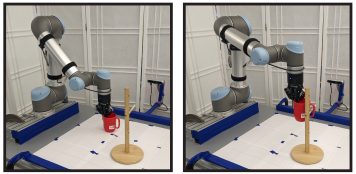
\includegraphics[width=0.45\textwidth]{figures/mugs1.png} \\
    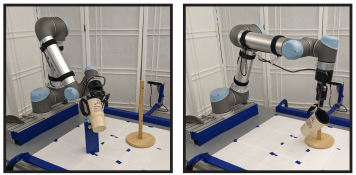
\includegraphics[width=0.45\textwidth]{figures/mugs2.png}
    \end{center}
\vspace{-0.2cm}
\caption{The Mug Tree task.}
\label{fig:mugontree}
\end{wrapfigure}


In one shot imitation learning, we are given a single demonstration of a desired manipulation behavior and we must find a policy that can reproduce the behavior in different situations. The classic example of this is the Mug Tree task where the robot must grasp a mug and hang it on a tree by its handle. Given a single demonstration of grasping a mug and hanging it on a tree (top row of Figure~\ref{fig:mugontree}), we want to obtain a policy that can successfully perform the same task for differently shaped objects placed in different poses, e.g. differently shaped mugs and trees (bottom row of Figure~\ref{fig:mugontree}). There are two key challenges here. First, the demonstration must generalize to novel object instances, e.g. different mugs. Second, the policy must reason in $SE(3)$ rather than in $SE(2)$ where the problem is significantly easier.

% A variety of effective approaches have been proposed for imitation learning in the plane, e.g.~\cite{}, but the problem in $SE(3)$ is much harder. 

To be successful in $SE(3)$, it is generally necessary to bias the model significantly toward the object manipulation domains in question. One popular method of accomplishing this is to use keypoints~\cite{pan2022tax,wang2019dynamic,manuelli2019kpam}. The idea here is to train a neural network model to assign descriptors to points on a novel object instance as a function of their semantic location on the object, e.g. points on the handles from different mugs would be assigned similar descriptors. Once these descriptors have been learned, they can be used to represent relative object poses for object categories in terms of the relative locations of their keypoints. This enables us to translate a demonstration on one of set of in-category objects to a different set of in-category objects. For example, the system would be able to translate the demonstration in the top row of Figure~\ref{fig:mugontree} to produce the behavior in the bottom row of Figure~\ref{fig:mugontree}.

Within the context of keypoint methods, a key challenge becomes how to learn semantically meaningful keypoint descriptors. This generally happens during a pretraining step where category-level object models are trained using a large number (generally hundreds) of in-category object instances for each category, e.g. hundreds of different instances of mugs. Different methods use different descriptor models. Early work used hand coded feature labels~\cite{manuelli2019kpam}. More recent methods learn descriptors as the byproduct of an implicit object model~\cite{simeonov2022neural}. Other methods learn a point embedding using a constrastive loss on a DGCNN~\cite{wang2019dynamic} model~\cite{pan2022tax}. The common thread here is that all of these methods involve a heavyweight category level object model that is trained on hundreds of objects to produce keypoint descriptors.

This paper proposes a different approach to the problem based on Coherent Point Drift (CPD)~\cite{myronenko2010point}, a point set registration algorithm. Using CPD, we train a shape completion model to register a novel in-category object instance to a canonical object model in which the a task has been defined via one-shot demonstration. The canonical task can then be projected into scenes with novel in-category objects by registering the new objects to the canonical models. Our method has several advantages over the previous work mentioned above~\cite{pan2022tax,wang2019dynamic,manuelli2019kpam}. First, it performs better, both in simulation and on robotic hardware, in terms of its ability to successfully perform a novel instance of a demonstrated task. Second, it requires an order of magnitude fewer object instances to train each new object category -- tens of object instances rather than hundreds. Third, our method is completely devoid of neural networks -- the approach is based on Gaussian Mixture models instead. This makes the approach more computationally efficient and it means that it is much easier to reason about issues like uncertainty and safety of the model. 


% \subsection{Old Intro}

% Robot learning of manipulation policies in the open world -- in situations, and to objects, the robot has not previously encountered -- is a grand challenge in robotics. An important aspect of this problem is our representation of the 3D world. Our paper focuses on a factored representation of the world, where we first find all objects of interest and then represent the 3D shape of each object independently. Our representation should generalize to unfamiliar objects in unfamiliar environments. For example, a robot should be able to enter a new kitchen and place a mug of a new shape on a hook (Figure \ref{fig:intro}). Additionally, we wish the robot to generalize to objects placed in novel positions and orientations. E.g. the robot should be able to pick a mug laying sideways on a floor even if it has previously only seen mugs standing on a countertop. We call this property $\mathrm{SE}(3)$-equivariance.

% Classical robotics approaches represent objects using explicit 3D geometries. \citet{miller03automatic,tenorth13decomposing} decompose complex objects into primitive shapes to plan for grasps and \citet{klank09realtime,beetz11robotic} rely on having CAD models of all objects in the world. The generalization ability of these approaches is limited, as these hand-crafted 3D representations cannot be accurately fit to any new object the robot encounters. To address this limitation, recent approaches use implicitly learned 3D descriptors. \citet{mescheder19occupancy,park19deepsdf} represent the 3D surface of an object as a decision boundary of a binary classifier neural network. Each 3D point nearby the surface of the object can then be described using the activations of the neural network \cite{simeonov22neural}. \citet{pan22taxpose} use neural point cloud embeddings \cite{qi17pointneta} and cross-attention \cite{vaswani17attention} to learn point cloud representations that are comparable between object instances.

% Implicit 3D descriptors have led to impressive results in few-shot 3D manipulation. Neural Descriptor Fields (NDFs) \cite{simeonov22neural,simeonov22se} and TAX-Pose \cite{pan22taxpose} learn object re-arrangement policies, e.g. hanging a mug on a hook, from 5 - 10 demonstrations. NDFs use 3D descriptors to match task-relevant object parts between different instances of objects. For example, they align the handles of differently shaped mugs in order to successfully hang them. Alternatively, Tax-Pose computes the cross-attention between the child (mug) and the parent (hook) objects in order to find which parts of the two objects should be nearby each other in the target configuration (mug on tree). The direct comparison between the child and the parent objects can lead to higher accuracy than in NDFs. But, both NDFs and Tax-Pose have two important limitations: (1) a large collection of 3D meshes is required for pre-training (200 objects per category from ShapeNet \cite{chang15shapenet}) and (2) without explicit 3D geometries, it is difficult to perform collision checking and motion planning on a physical robot.

% Our paper focuses on an alternative and highly sample-efficient explicit 3D geometry representation method based on \textit{shape warping} \citep{jakel12learning,brandi14generalizing,lee15learning,schulman16learning,rodriguez18transferring,rodriguez18transferringa,thompson21shapebased}. The core idea is to pick a canonical example of an object class, and warp its point cloud (or mesh) to conform to the observations of novel object instances \cite{myronenko10pointset,hillenbrand12transferring,benamor12generalization}. The immediate benefit is that we do not have to represent the shape of an object, but only the \textit{displacement} of points as they are warped between different object instances (belonging to the same object class). We base our method on prior work by \citet{rodriguez18transferring,thompson21shapebased}, who propose to use gradient-descent-based inference to enable shape warping to partial point clouds.
% % \tk{We base our method on ... [or mention this connection later in the method section, might not be needed here]} 

% We propose \textbf{Shape and Action Warping (SA-Warp)}, a general method for one-shot learning of robotic manipulation policies. First, we propose a new algorithm for the joint inference of object shape, scale, translation and orientation based on its partial point cloud. The algorithm is based on canonical object warping with a low-dimensional latent space of shapes \cite{rodriguez18transferring,thompson21shapebased} and returns a warped 3D mesh. Second, we propose a method for the warping of robot actions. We focus on actions where two objects come into contact: e.g., grasping, relative object placement (e.g. mug on tree) and trajectory cloning with contacts (e.g. painting with a brush on a canvas). Our method finds the \textit{interaction points} between pairs of objects, anchors them to their canonical counterparts, and warps them to conform to objects of novel shapes. We developed SA-Warp specifically for on-robot behavior cloning, and we extensively test it in real-world robot experiments.

\section{Related Work}

\subsection{Imitation Learning from Few Demonstrations} 

We build on a body of robotics work aimed at learning generalizable manipulation policies from few demonstrations. A seminal idea in the literature is a key-point-based representation of objects. \citet{manuelli19kpam} manually create a dataset of semantically meaningful key-points, such as the rim and the handle of a mug, and train a classifier to detect key-points on novel object instances. A task is defined as a time series of key-point positions. Then, a trajectory for a previously unseen object can be computed by matching the key-points on the novel object to the key-point positions seen in a demonstration. In comparison, our method does not require a manual labeling of key-points -- we use the inferred geometry of objects to automatically extract interaction points. \citet{gao21kpam,gao21kpamsc} further extend the key-point framework with feedback control and collision checking. ... also ... \cite{1910,vecerik20s3k,manuelli20keypoints,turpin21gift}.

A related idea is the learning of descriptors attached to arbitrary 2D or 3D key-points. \citet{florence18dense} use self-supervised learning to learn dense descriptors from images. These descriptors can be used to compute similarities of arbitrary key-points between different instances and poses of objects. \citet{chen22neural} compute descriptors of an arbitrary 3D coordinate, called Neural Descriptor Fields, using an implicit shape representation neural network conditioned on a point cloud \cite{mescheder19occupancy}. By attaching a pose of an object to a set of descriptors, they can match e.g.~the pose of a handle of a mug across different mug instances and poses. The method is used re-arrange objects with a variable initial pose and a fixed goal. \citet{simeonov22se} represent pairs of objects using Neural Descriptor Fields to enable generalization across goal poses. \citet{chun23local} further leverage the locality bias of Neural Descriptor Fields to generalize demonstrations across object classes.

Some works rely on CAD model matching to reproduce grasps or manipulation trajectories  \cite{klank09realtime,brook11collaborative,beetz11robotic,jakel12learning}. ... also shape primitives \cite{miller03automatic} ... But, it can be difficult to generalize these methods to novel instances of objects. Recently, \citet{wen22you} tackled category-level manipulation by re-mapping key poses of objects across instances. \citet{pan22taxpose} make predictions about the desired pose of a child object related to a parent object (e.g. hanging a mug on a mug-tree) using cross-attention \cite{vaswani17attention} between the pair of point clouds.


\subsection{Shape Warping and Manipulation}

Prior works explored the idea of learning a generative model of point clouds through non-rigid point cloud registration \cite{rodriguez18transferring,rodriguez18transferringa,klamt18supervised,thompson21shapebased}. The model is used to grasp objects based on partial point clouds \cite{rodriguez18transferring,rodriguez18transferringa,klamt18supervised} and to parameterize motion primitives \cite{thompson21shapebased}. In contrast, we learn a generative model of meshes, which we use to find interaction points in demonstrations of manipulation tasks, which in turn enable generalization across object instances. In addition, the pose of objects is either assumed to be given \cite{thompson21shapebased} or detected using a neural pose detector \cite{klamt18supervised}. We propose joint shape and pose inference using gradient descent with random restarts. Gradient descent on both the pose and the shape was used in \cite{rodriguez18transferring,rodriguez18transferringa}, but only to correct for minor deviations in pose. ... also \cite{simeonov20long,you21omnihang,menon22viewpoint,lu22online,wen22you,cong23comprehensive} ...

A second related line work is focused on detecting the contacts between a gripper and an object, and then warping the contact points to fit a novel object \cite{li07datadriven,benamor12generalization,hillenbrand12transferring,jakel12learning,stouraitis15functional,rodriguez18learning,pavlichenko19autonomous,tian19transferring} ... and others ... Instead of directly warping the contact points, we first register them on the canonical mesh corresponding to the grasped object class. This way, we can predict grasps based on partial point clouds; we can even grasp a part of the object that is visually occluded. \ob{I could make a figure for this.}

Finally, point cloud warping has been used to manipulate deformable objects \cite{lee15learning,schulman16learning} and to parameterize a pouring skill \cite{brandi14generalizing}.


%-- \cite{rodriguez18transferring,rodriguez18transferringa}: Similar to Skye's method; they learn a latent space of displacements w.r.t. a canonical point cloud using PCA. During inference, they use gradient descent to solve for both shape and pose. But, they do not tackle the problem of local minima and hence require the shapes to be already almost in alignment. I could give the example of a handle of a mug getting hidden because of local minima and how we solve that. They then use the latent space to somehow warp the grasp actions of a humanoid hand.

\section{Background: Shape Warping by CPD and Gradient Descent}
\label{sec:background}

\begin{figure}
    \centering
    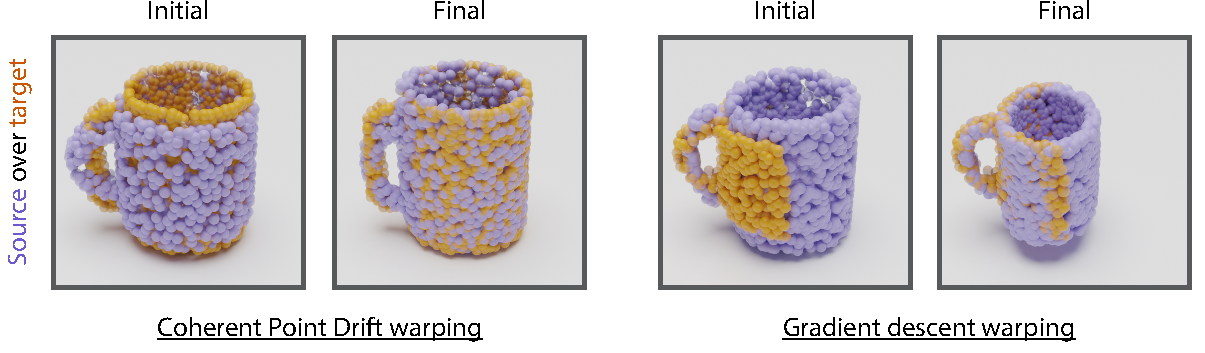
\includegraphics[width=\textwidth]{figures/warping.pdf}
    \caption{Example of warping using CPD and gradient descent with a latent space of warps of a canonical mug. Gradient descent warping works with partial point clouds.}
    \label{fig:warping}
\end{figure}

Shape warping aims to find the correspondence between the shape of two objects by altering one shape to fit the other (Figure \ref{fig:warping}). Usually, the first step is to turn both objects into point clouds. This can be accomplished by sampling the surface or the volume of the object, or directly using the vertices that make up the mesh of the object. Given a pair of point clouds to be matched, shape warping draws on the literature of non-rigid point cloud registration \cite{huang21comprehensive}. Next, we outline the Coherent Point Drift algorithm \cite{manuelli20keypoints}, a common method for aligning a pair of point clouds. We also introduce the necessary notation we will use throughout the paper.
%\rob{This section is not nearly as clear as it should be. You should describe CPD as if you were teaching the method to someone who is new to it. The section is a little short; but most importantly, you introduce new notation when it seems unnecessary and present ideas in a way that makes it hard to follow.}

Denote a pair of point clouds $\pci$ and $\pcj$. We want to compute a matrix of displacements $\wij$ that minimizes some distance function between $\pci + \wij$ and $\pcj$, such as the one-sided Chamfer distance:
\begin{align}
    d\left( \pci + \wij, \pcj \right) = \frac{1}{|\pcj|} \sum_{k=1}^{|\pcj|} \min_{l=1}^{|\pci|} \norm{ \pci_l + W_{i \rightarrow j, l} - \pcj_k }_2.
\end{align}
Note that the two point clouds can have a different number of points. In general, $\wij$ can re-arrange $\pci$ in an arbitrary way, leading to a mapping that is not useful. The Coherent Point Drift (CPD) algorithm regularizes $\wij$ so that nearby points in $\pci$ are displaced similarly. CPD formulates the problem as a fitting of a Gaussian Mixture Model (GMM), where $\pci$ is a set of components and $\pcj$ is the data. It uses expectation maximization to optimize the objective function
\begin{align}
    J(\wij) = - \sum_{k=1}^{|\pcj|} \log \sum_{l=1}^{|\pci|} \exp \left( \frac{1}{2 \sigma^2} \norm{\pcj_k - (\pci + \wij)_l} \right) + \frac{\alpha}{2} \phi(\wij).
\end{align}
The regularizer $\phi$ penalizes high frequencies in $\wij$, so that the displacements applied to $\pci$ do not oscillate among nearby points.

\citet{rodriguez18transferring} observed that we can treat each displacement matrix $\wij$ as a data point in order to learn a generative model of object shapes. Given a canonical object $\pcc$ and a set of warps $\{ \wci \}_{i=1}^K$, each matrix $\wci$ is flattened and treated as a feature vector. Then, we fit a PCA projection matrix $W \in \mathbb{R}^{|\pcc|{\times}D}$ to the data, which allows us to represent each shape by a low-dimensional latent vector $v$:
\begin{align}
    \pcx{v} = \pcc + W v.
\end{align}
Given a new point cloud $\pci$, we infer its shape by solving the following optimization problem by gradient descent:
\begin{align}
    v^* = \argmin_{v \in \mathbb{R}^D} d(\pcc + W v, \pci).
\end{align}
Finally, the term $Wv$ can be replaced by a more expressive model, e.g. an auto-encoder \cite{thompson21shapebased} or possibly a diffusion model \cite{nichol22pointe}. We use PCA for simplicity.

\section{Interaction Warping (IW)}

% \begin{figure}
%     \centering
%     \includegraphics[width=\textwidth]{figures/method_figure2.pdf}
%     \caption{Main method figure. I'll fill it in with real-world images later. \rob{I'm thinking instead of a fig that focuses on warping of relative pose between pair of objects. Maybe visualize mug-on-tree (or bottle in box) for diff warped configs, similar to what you do in fig 2 for objects.}}
%     \label{fig:method}
% \end{figure}

In this section, we propose \textbf{Interaction Warping (IW)}, a method for imitation learning using shape warping. IW is robust to shape variation between object instances and sample-efficient in terms of both the number of example objects and the number of demonstrations of  a task. Our method has three main components that make it work on a real-world robot: (1) hybrid mesh and point cloud warping to enable the detection of contact points and collision avoidance during motion planning, (2) joint estimation of object shape and pose in 3D using gradient descent and (3) warping of interactions between objects (including the robot gripper) to enable the transfer of 3D robot actions across object instances.

\subsection{Latent Space of Meshes}
\label{sec:methods:mesh}

\begin{figure}
    \centering
    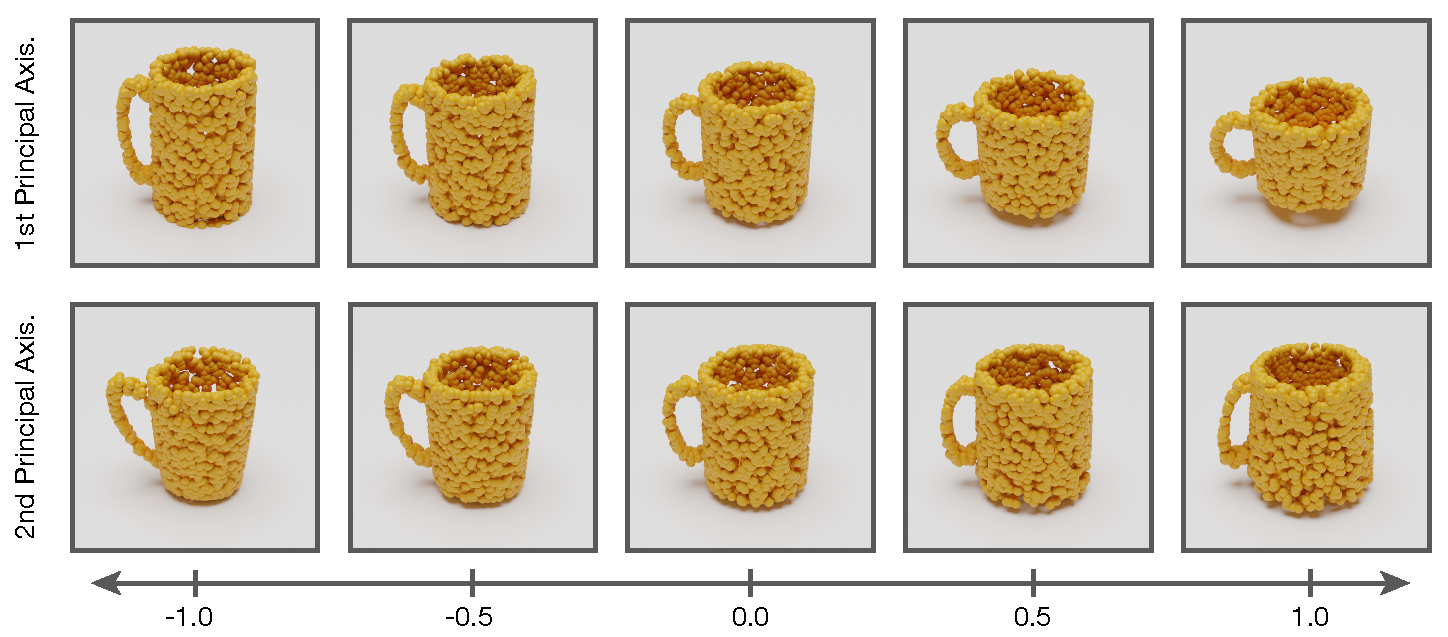
\includegraphics[width=\textwidth]{figures/latent_mugs2.pdf}
    \caption{The first two principal components of a latent space of mug warps.}
    \label{fig:latent}
\end{figure}

We pre-train IW with a small number of example objects (ten objects from ShapeNet \cite{chang15shapenet} in our experiments) for each object class. We assume to have access to object meshes and we sample a point cloud per object using surface sampling. For each class, we select a canonical example $C$ that appears to be the most representative (we describe two possible heuristics in Appendix \ref{appendix:method:canonical}). Then, we apply the method of \cite{rodriguez18transferring} described in Section \ref{sec:background} to learn a latent space of object warps (Figure \ref{fig:latent}). As a result, we can parameterize object shape by a low-dimensional vector $v$:
\begin{align}
    \pcx{v} = \pcc + W v. \tag{3}
\end{align}

For real-world applications, we found it important to have access to the surface of the object shape parameterized by $v$ in addition to its point cloud. If the point cloud of $\pcx{v}$ is dense enough, it is possible to use surface completion methods. But, we found a simpler approach to work well: we construct the canonical point cloud $\pcc$ as a concatenation of the actual vertices of object $C$ and points sampled on its surface. By having actual vertices in $\pcc$, we ensure that they can be warped to create a new mesh. We add the surface samples to make the point cloud more uniform -- meshes modeled by people tend to have highly non-uniform distributions of vertices.

Finally, we create a new mesh by extracting the warped vertices from $\pcx{v}$ and keeping the original faces (represented as triplets of vertex indices) from object $C$. This way of warping vertices can possibly break the mesh (e.g. by intersecting or inverting its faces), but we did not find it to be a problem when performing collision checking for a reasonable range of real-world objects.

\subsection{Fitting a Mesh to the Observed Point Cloud}
\label{sec:methods:scene}

We observe real-world (or simulated) point cloud $\mathrm{scene\_pcd}$ using one to three RGB-D cameras. The cameras are calibrated to the robot's hand and we fuse their outputs into a single point cloud. We detect each object of interest in $\mathrm{scene\_pcd}$ either using clustering and heuristics (Section \ref{sec:exp:rearrangement}) or using pre-trained RGB-based open-vocabulary object detection and instance segmentation models (Section \ref{sec:exp:wild}).

Using our latent space from Section \ref{sec:methods:mesh}, we aim to recover the pose and the complete mesh of each detected object from its point cloud $\mathrm{pcd}$. First, we use the class of the detected object to select a model from Section \ref{sec:methods:mesh} -- we have one for each class. We center $\mathrm{pcd}$ and initialize the canonical point cloud with the following parameters:
\begin{align}
    v = \begin{pmatrix} 0 & 0 & ... & 0 \end{pmatrix}, s = \begin{pmatrix} 1 & 1 & 1 \end{pmatrix}, t = \begin{pmatrix} 0 & 0 & 0 \end{pmatrix}, r = \begin{pmatrix} 1 & 0 & 0 \\ 0 & 1 & 0 \end{pmatrix}.
\end{align}
The point clouds starts in its canonical form with the latent shape $v$ equal to zero. We set the initial scale $s$ to one, translation $t$ to zero and rotation $r$ to a unit rotation matrix. We use the Gram-Schmidt orthogonalization process to turn the six entries in $r$ into a proper 3D rotation matrix $R$. This method has been shown to enable stable learning of rotation matrices \cite{falorsi18explorations, park22learning}.

We decode the shape and pose parameters into a transformed point cloud
\begin{align}
    \mathrm{dec} = [(\pcc + W v) \odot s] R^T + t,
\end{align}
and define a loss function
\begin{align}
    \mathcal{L}(\mathrm{dec}) = \underbrace{\frac{1}{|\mathrm{pcd}|} \sum_k^{|\mathrm{pcd}|} \min_l^{|\mathrm{dec}|} \norm{\mathrm{pcd}_k - \mathrm{dec}_l}_2^2}_{\text{(1)}} + \underbrace{\beta \max_l^{|\mathrm{dec}|} \norm{\mathrm{dec}_l}_2^2}_{\text{(2)}}.
\end{align}
The first term in the loss function is a one-sided Chamfer distance between the decoded and the observed point clouds. The second term is a regularizer on the size of the decoded object. Our implementation regularizes the object to fit into the smallest possible ball. Other options are possible, such as directly regularizing $v$ and $s$, regularizing the $L_2$ norm of $\mathrm{dec}$, etc. The main reason for the regularizer is to prevent large predicted meshes in real-world experiments, which might make it impossible to find collision-free motion plans.

We minimize $\mathcal{L}$ with respect to $v, s, t$ and $r$ using the Adam optimizer \cite{kingma17adam} with learning rate $10^{-2}$ for 100 steps. We set $\beta=10^{-2}$. We found the optimization process is prone to getting stuck in local minima; e.g., instead of aligning the handle of the decoded mug with the observed point cloud, the optimizer might change the shape of the decoded mug to hide its handle. Hence, we restart the process with many different random initial rotations and pick the solution with the lowest loss function. Further, we randomly subsample the point clouds at each gradient descent step -- this allows us to run 12 random starting orientations at once on a consumer GPU.

As a result, we get the decoded point cloud $\mathrm{dec}$ (turned into a mesh as described in Section \ref{sec:methods:mesh}) and its pose represented by $t$ and $R$.

\subsection{Cloning Robot Actions via Interaction Points}

\begin{figure}
    \centering
    \begin{subfigure}[b]{0.25\textwidth}
        \centering
        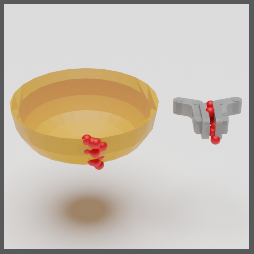
\includegraphics[width=\textwidth]{figures/contact_fig1.pdf}
        \caption{}
    \end{subfigure}
    \hspace{0.05\textwidth}
    \begin{subfigure}[b]{0.25\textwidth}
        \centering
        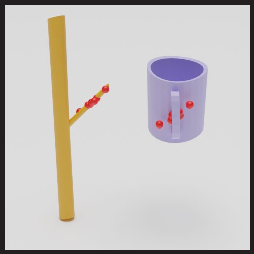
\includegraphics[width=\textwidth]{figures/contact_fig3.pdf}
        \caption{}
    \end{subfigure}
    \hspace{0.05\textwidth}
    \begin{subfigure}[b]{0.25\textwidth}
        \centering
        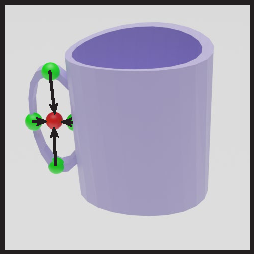
\includegraphics[width=\textwidth]{figures/contact_fig2.pdf}
        \caption{}
    \end{subfigure}
    \caption{(a) Contacts between a gripper and a bowl extracted from a demonstration. (b) Nearby points between a mug and a tree extracted from a demonstration of hanging the mug on the tree. (c) A virtual point (red) representing the branch of the tree intersecting the handle of the mug. The red point is anchored to the mug using k nearest neighbors on the mug (four are shown in green) and moves as the mug warps. All points shown in this visualization are extracted automatically.} % \ob{TODO: The red point on the mug in (b) are pointing in the wrong way.}
    \label{fig:contacts}
\end{figure}

\begin{figure}
    \centering
    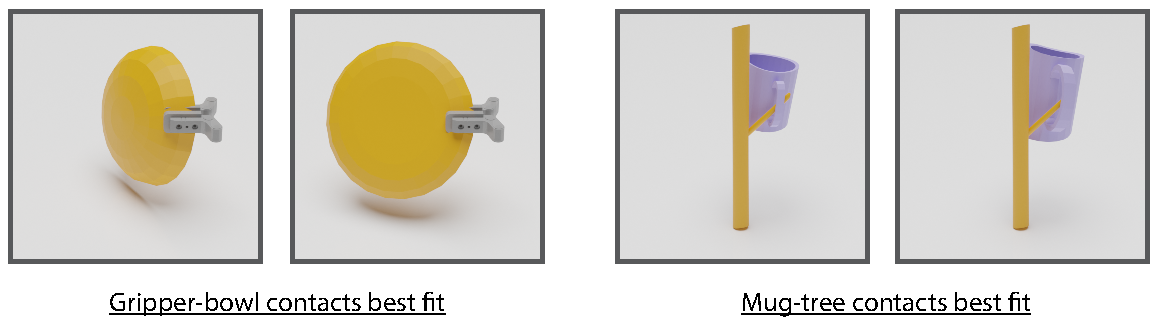
\includegraphics[width=\textwidth]{figures/picks_and_places.pdf}
    \caption{Predicting grasps using interaction point warping. (a) the predicted grasp for a bowl/plate changes based on the curvature of the object. (b) the placement of a mug on a mug tree changes as the mug grows larger so that the branch of the tree is in the middle of the handle.}
    \label{fig:grasps_and_placements}
\end{figure}

Our key contribution is a generalizable representation of 3D robotic actions with respect to manipulated objects. We propose an action abstraction we call \textit{interaction points}: pairs of these points capture the interaction of either a robot and an object, or a pair of objects. Crucially, we are able to warp interaction points to novel objects without any additional learning. We describe the cloning of grasping and relational object placement, but interaction points could be also used in, e.g., pushing or tossing. We use a single demonstration of a grasp or a placement to identify the interaction points.

\textbf{Grasping:} Assume that we have a single demonstration of grasping an object. We have inferred object shape $v$ and pose $T$ (Section X). We also have our reconstructed and transformed point cloud $\pcx{v}$, object mesh $\mathrm{obj}^{(v)}$ and a gripper mesh $\mathrm{grip}$. We find $N$ pairs of points $(p^{(v)}_j, p^{(G)}_j)$ that define the contacts between the object and the gripper. We use \texttt{pybullet} collision checking for this purpose. Each $p^{(v)}_j$ is a point in $\pcx{v}$ with index $i_j$.

Given a new object to be grasped with shape $v'$, pose $T'$ and a point cloud $\pcx{v'}$, we create new pairs of points $(p^{(v')}_i, p^{(G)}_i)$. The points $p^{(v)}_i$ and $p^{(v')}_i$ are related by the following equation:
\begin{align}
    p^{(v')}_j T'^{-1} = \underbrace{p^{(v)}_j T^{-1}}_{\text{(1)}} + \underbrace{[W(v' - v)]_{i_j}}_{\text{(2)}} \label{eq:contact_point_warping}.
\end{align}
Intuitively, we transform the interaction points to a canonical pose and then warp them to conform to a new object instance. Term 1 ensures that we can repeat the grasp in any orientation ($\mathrm{SE}(3)$-invariance) and Term 2 encodes generalization over object shapes using linear shape warping.

We compute the target pose of the robot gripper as the optimal transform $T_{\text{grasp}}$ of the points $p^{(G)}_j$ that minimizes the following loss function. An analytical solution exists \cite{horn88computation}.
\begin{align}
    \mathcal{L}(T) = \sum_{j=1}^N \norm{ p^{(v')}_j - T p^{(G)}_j }_2^2. \label{eq:coordinate_transform}
\end{align}

\textbf{Relational object placement:} We consider tasks where object 1 should be placed in a specific configuration relative to object 2. The placement can be both final (e.g. mug on mug-tree) on only a waypoint in a task (e.g. brush sliding over a canvas). Given a demonstration, we infer the pose $T_1, T_2$ and shape $v_1, v_2$ of both objects as well as their reconstructed and transformed point clouds $\pcx{v_1}, \pcx{v_2}$. We find all pairs of nearby points $(p^{(v_1)}_j \in \pcx{v_1}, p^{(v_2)}_j \in \pcx{v_2})$ such that $\norm{p^{(v_1)}_j - p^{(v_2)}_j} \leq \delta$. This step will usually return thousands of points and we find a subset of size 100 using farthest point sampling \cite{eldar94farthest} to get a representative sample. We use nearby points as a strict generalization of contact points: some demonstrations of a task can involve placing an object free of contact and letting it fall in place.

Since $p^{(v_1)}_j$ and $p^{(v_2)}_j$ are not necessarily in contact, we cannot simply compute the optimal transform that aligns the pairs of points. We solve this problem by creating virtual points in $\pcx{v_1}$ that are in contact with points $p^{(v_2)}_j$. Each virtual point is defined as
\begin{align}
    p^{(v_1)}_{V,j} = \frac{1}{L} \sum_{k=1}^L \pcx{v_1}_{i_k} + \underbrace{(p^{(v_2)}_j - \pcx{v_1}_{i_k})}_{\Delta_k} = p^{(v_2)}_j,
\end{align}
where $i_1, i_2$, ..., $i_L$ are indices of the k-nearest-neighbors to point $p^{(v_2)}_j$ in $\pcx{v_1}$. Figure \ref{fig:contacts} (b) and (c) shows an example of this process: we create a virtual points in the middle of the handle of a mug, which is in contact with the branch of a mug-tree. Note that these points are found automatically and we do not require any task specific information.

We now have pairs of points $(p^{(v_1)}_{V,j} \in \pcx{v_1}, p^{(v_2)}_j \in \pcx{v_2})$ that are in contact. Given a novel object 1 of shape $v'_1$, we can warp the virtual points as follows:
\begin{align}
    p^{(v'_1)}_{V,j} = \frac{1}{L} \sum_{k=1}^L \pcx{v'_1}_{i_k} + \Delta_k.
\end{align}
We can also warp the second object to shape $v'_2$ using Equation \ref{eq:contact_point_warping} and compute the new optimal transform $T_{\text{rel}}$ using Equation \ref{eq:coordinate_transform}. Finally, we transform $T_{\text{rel}}$ from the coordinate space of object 1 to the coordinate space of the gripper holding the object (we record the relative transform between the pose of the object and the gripper when we pick it up). Hence, we get $T_{\text{place}}$ that can be executed by a physical robot.


% \subsection{Action: Warping of Grasps and Placements}
% \label{sec:methods:cloning}

% In this section, we describe our approach to clone pick and place actions for different object shapes and poses, given a single demonstration of a task. In general, the demonstration consists of a sequence of $T$ \evdp{is this symbol overloaded? Earlier in the paper capital T (with subscript) referred to transformations} pick and place actions manipulating $M$ objects. Our experiments are restricted to $T=M=2$, but our algorithm is immediately applicable to any sequence, as long as it is told which object to manipulate at which time step. We record the pose of the gripper and the inferred object shape and pose (using Algorithm \ref{alg:warp_infer}):
% \begin{align}
%     \left(T_{\text{pick/place}}, (v_k, T_k)_{k=1}^M\right)_{t=1}^T
% \end{align}

% \textbf{Grasp cloning:} To clone a grasp, we register contact points between the gripper and an object. Since we infer the mesh $X$ of the grasped object using Algorithm \ref{alg:warp_infer}, we can sample $B$ contact points between the object mesh and the gripper mesh (Figure \ref{fig:warping}a). For each contact point, we find the nearest neighbor in $X$. We record these indices as $\left< i_1, i_2, ..., i_B \right>$.

% When transferring the grasp to a new scene with a different object instance in a different position and orientation, we denote the completed point cloud of the new instance as $Y$. Points $Y_{i_1}, Y_{i_2}, ..., Y_{i_B}$ correspond to the points the gripper touched when picking up the demo object. Since the points have been warped to a new instance, a new grasp could be required. We solve for the best fit between the contact points on $Y$ and the contact points on the gripper (we have pairs of points, where the first point is on the object and the second on the gripper) to get a new grasp pose (Figure \ref{fig:grasps_and_placements}).

% \textbf{Placement cloning:} We consider the placement of a child object $X_{\mathrm{child}}$ on a parent object $X_{\mathrm{parent}}$ (e.g. mug on tree, bottle in box) \evdp{what is the definition of a child vs a parent object?}. Given the inferred meshes, we could find the contact points between the child and the parent. However, the two objects might not always touch before the child object is released from the gripper. E.g., when putting an object into a container. Instead, we find nearby points between the child and the parent and anchor them to the child point cloud as \textit{virtual points}.

% \rob{Exactly the same comment here as in the grasp section. 1) define the points we're looking for; 2) What properties do these points need to have such that placement is guaranteed to be successful? 3) Does our method deliver? When and when not?}

% We find points $p_1, p_2, ..., p_B$ on the parent object that are nearby the child object (Figure \ref{fig:contacts}b). These points are again found based on the inferred meshes of the two objects. For the parent object, we find a nearest neighbor $X_{\mathrm{parent},i_j}$ for each point $p_j$ -- it is the same process as in grasp cloning. For the child object, we anchor each point $p_j$ to its point cloud using its $K$ nearest neighbors $(n_1, n_2, ..., n_k)$. We save the deltas between $p_j$ and its neighbors $\delta = (v_j - n_1, v_j - n_2, ..., v_j - n_k)$ (Figure \ref{fig:contacts}c). Given warped nearest neighbors $n'$, we update $p_j$ as the mean over the deltas to the neighbors:
% \begin{align}
%     p'_j = \frac{1}{k} \sum_{i=1}^k n'_i + \delta_i.
% \end{align}

% Using the above method, we can calculate pairs of contact points in a novel scene. We solve for the transformation of the child object so that the contact points are in the best possible alignment with the target object. Finally, we solve for a collision free motion plan that places the child object to the target pose.

\section{Experiments}
\label{sec:exp}

We evaluate both the perception and imitation learning capabilities of Interaction Warping. In Section \ref{sec:exp:rearrangement}, we perform three object re-arrangement tasks with previously unseen objects both in simulation and on a physical robot. In Section \ref{sec:exp:wild}, we show our system is capable of proposing grasps in a cluttered kitchen setting from a single RGB-D image.

\subsection{Object Re-arrangement}
\label{sec:exp:rearrangement}

\begin{figure}[]
    \centering

    \begin{subfigure}{(\linewidth - 0.05\linewidth)/5}
        \centering
        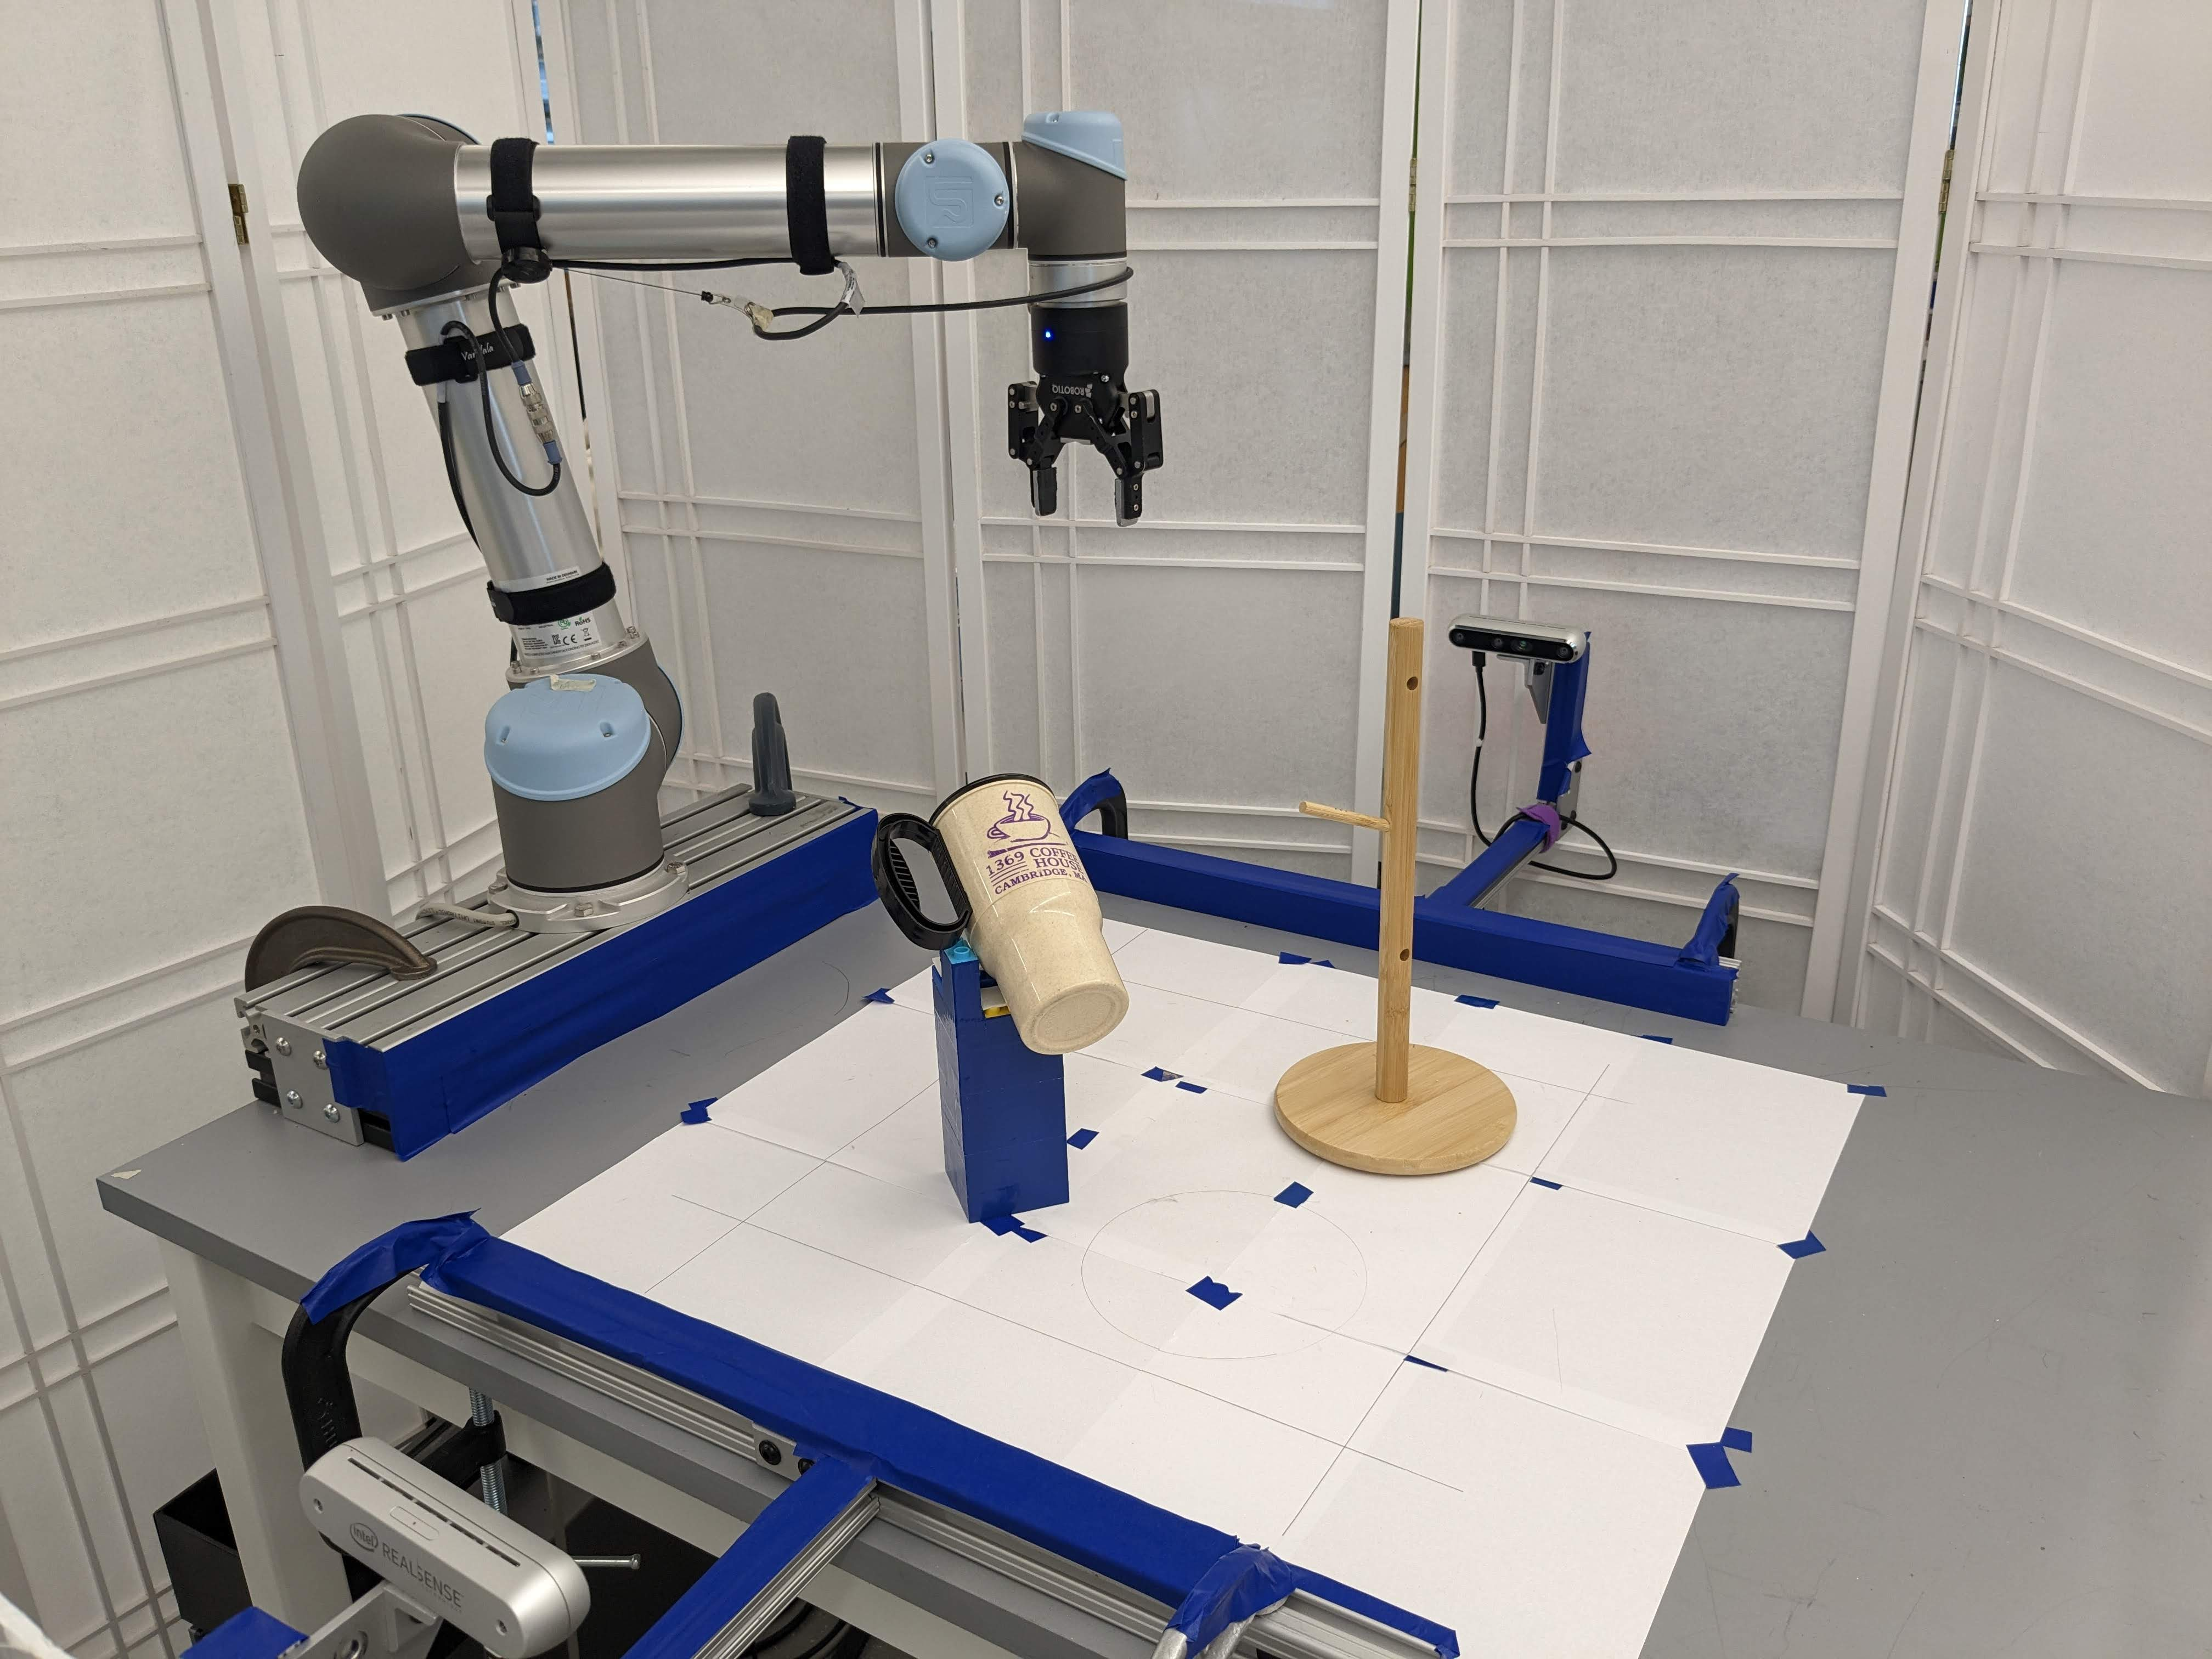
\includegraphics[width=\linewidth]{figures/episodes/mug_on_tree/1.jpg}
    \end{subfigure}
    \begin{subfigure}{(\linewidth - 0.05\linewidth)/5}
        \centering
        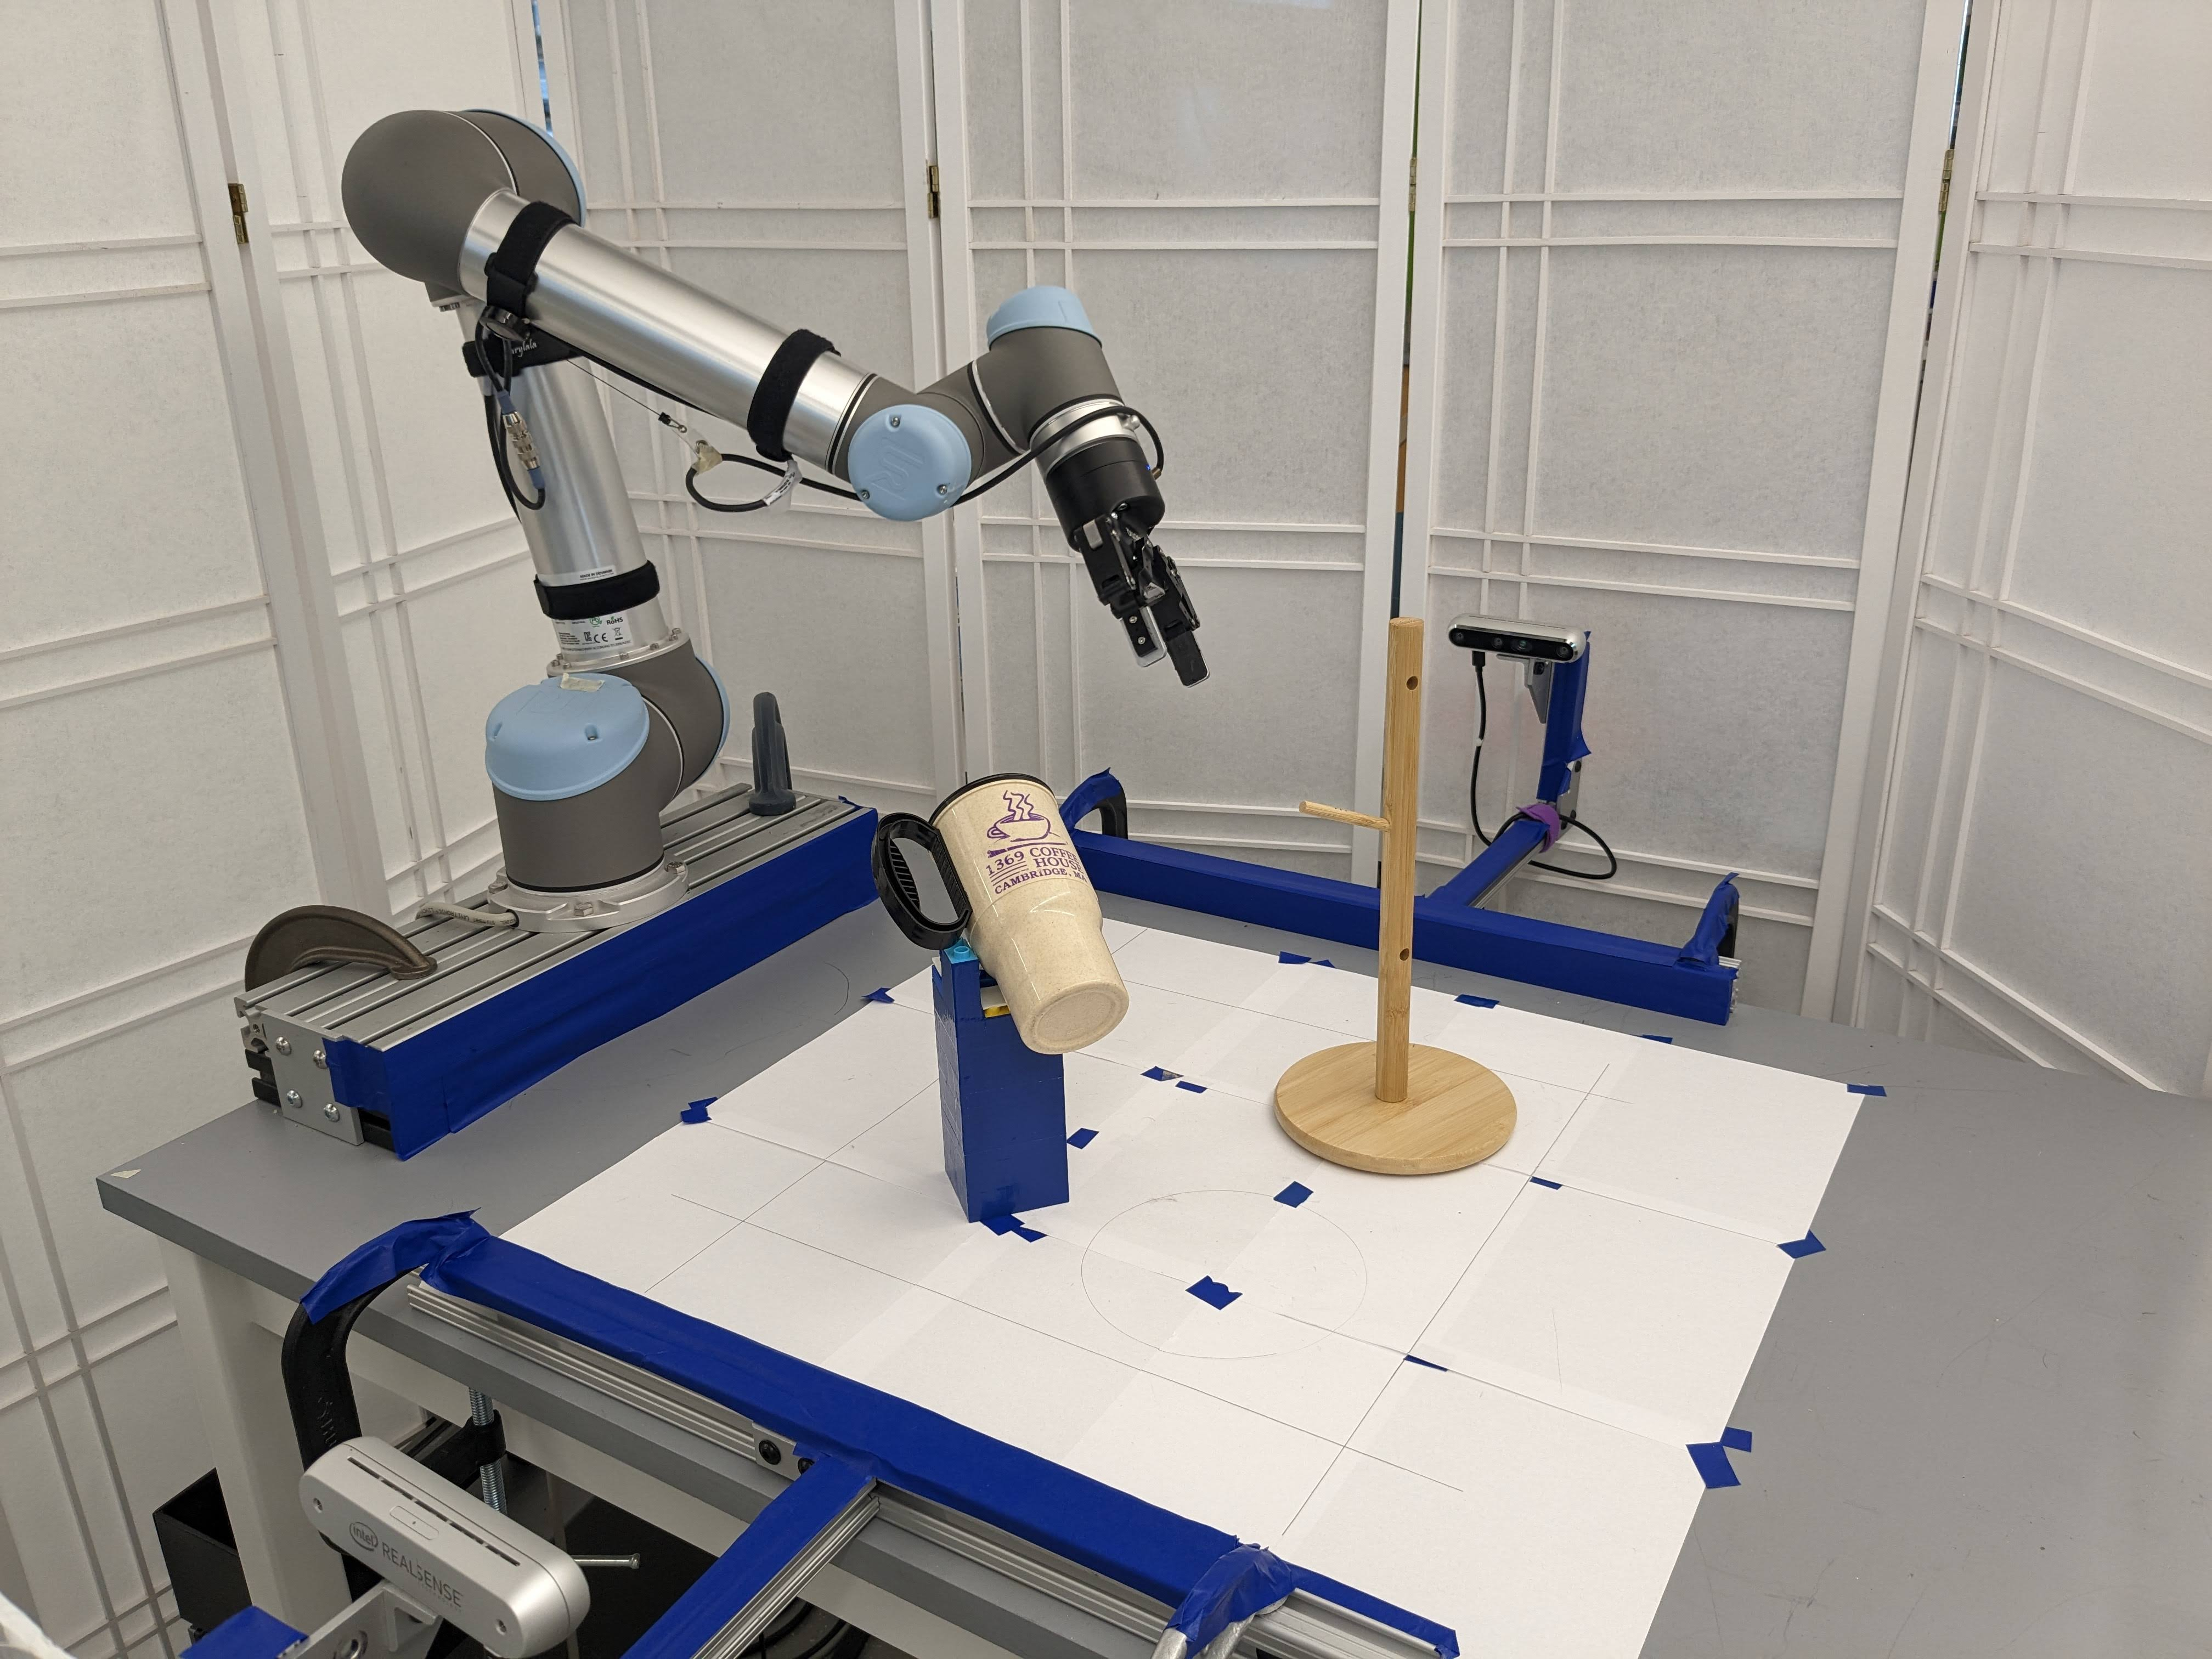
\includegraphics[width=\linewidth]{figures/episodes/mug_on_tree/2.jpg}
    \end{subfigure}
    \begin{subfigure}{(\linewidth - 0.05\linewidth)/5}
        \centering
        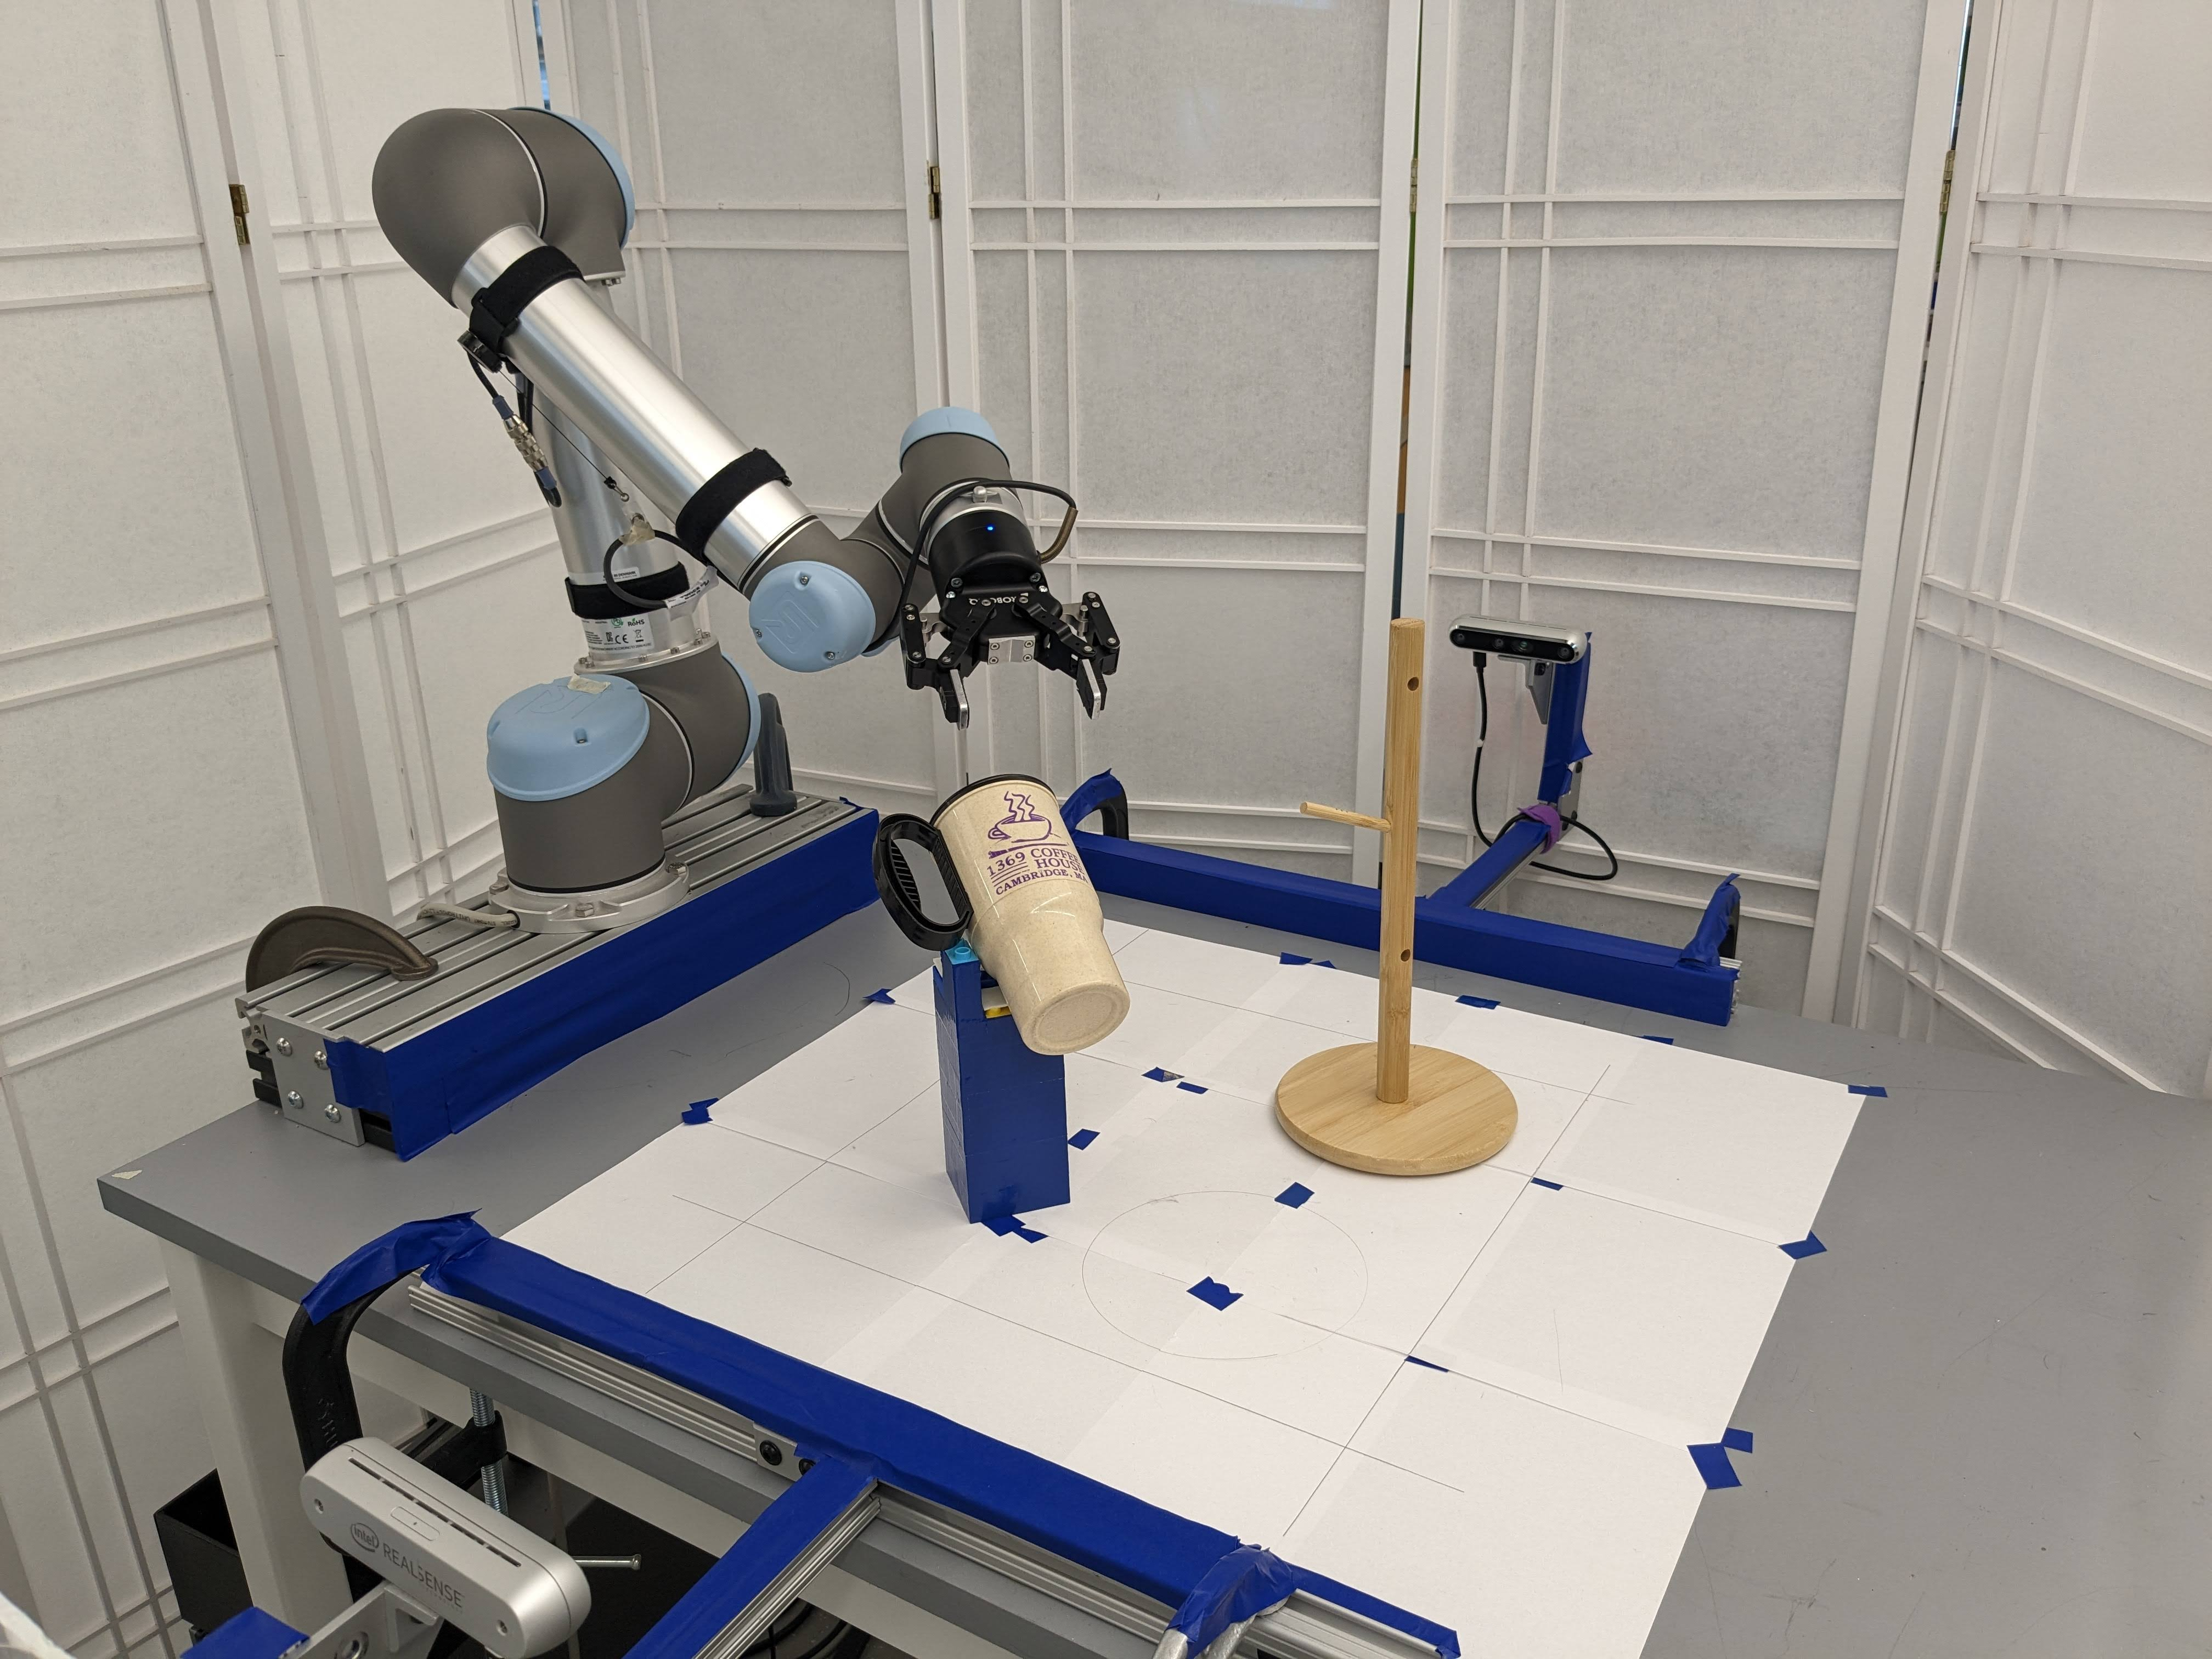
\includegraphics[width=\linewidth]{figures/episodes/mug_on_tree/3.jpg}
    \end{subfigure}
    \begin{subfigure}{(\linewidth - 0.05\linewidth)/5}
        \centering
        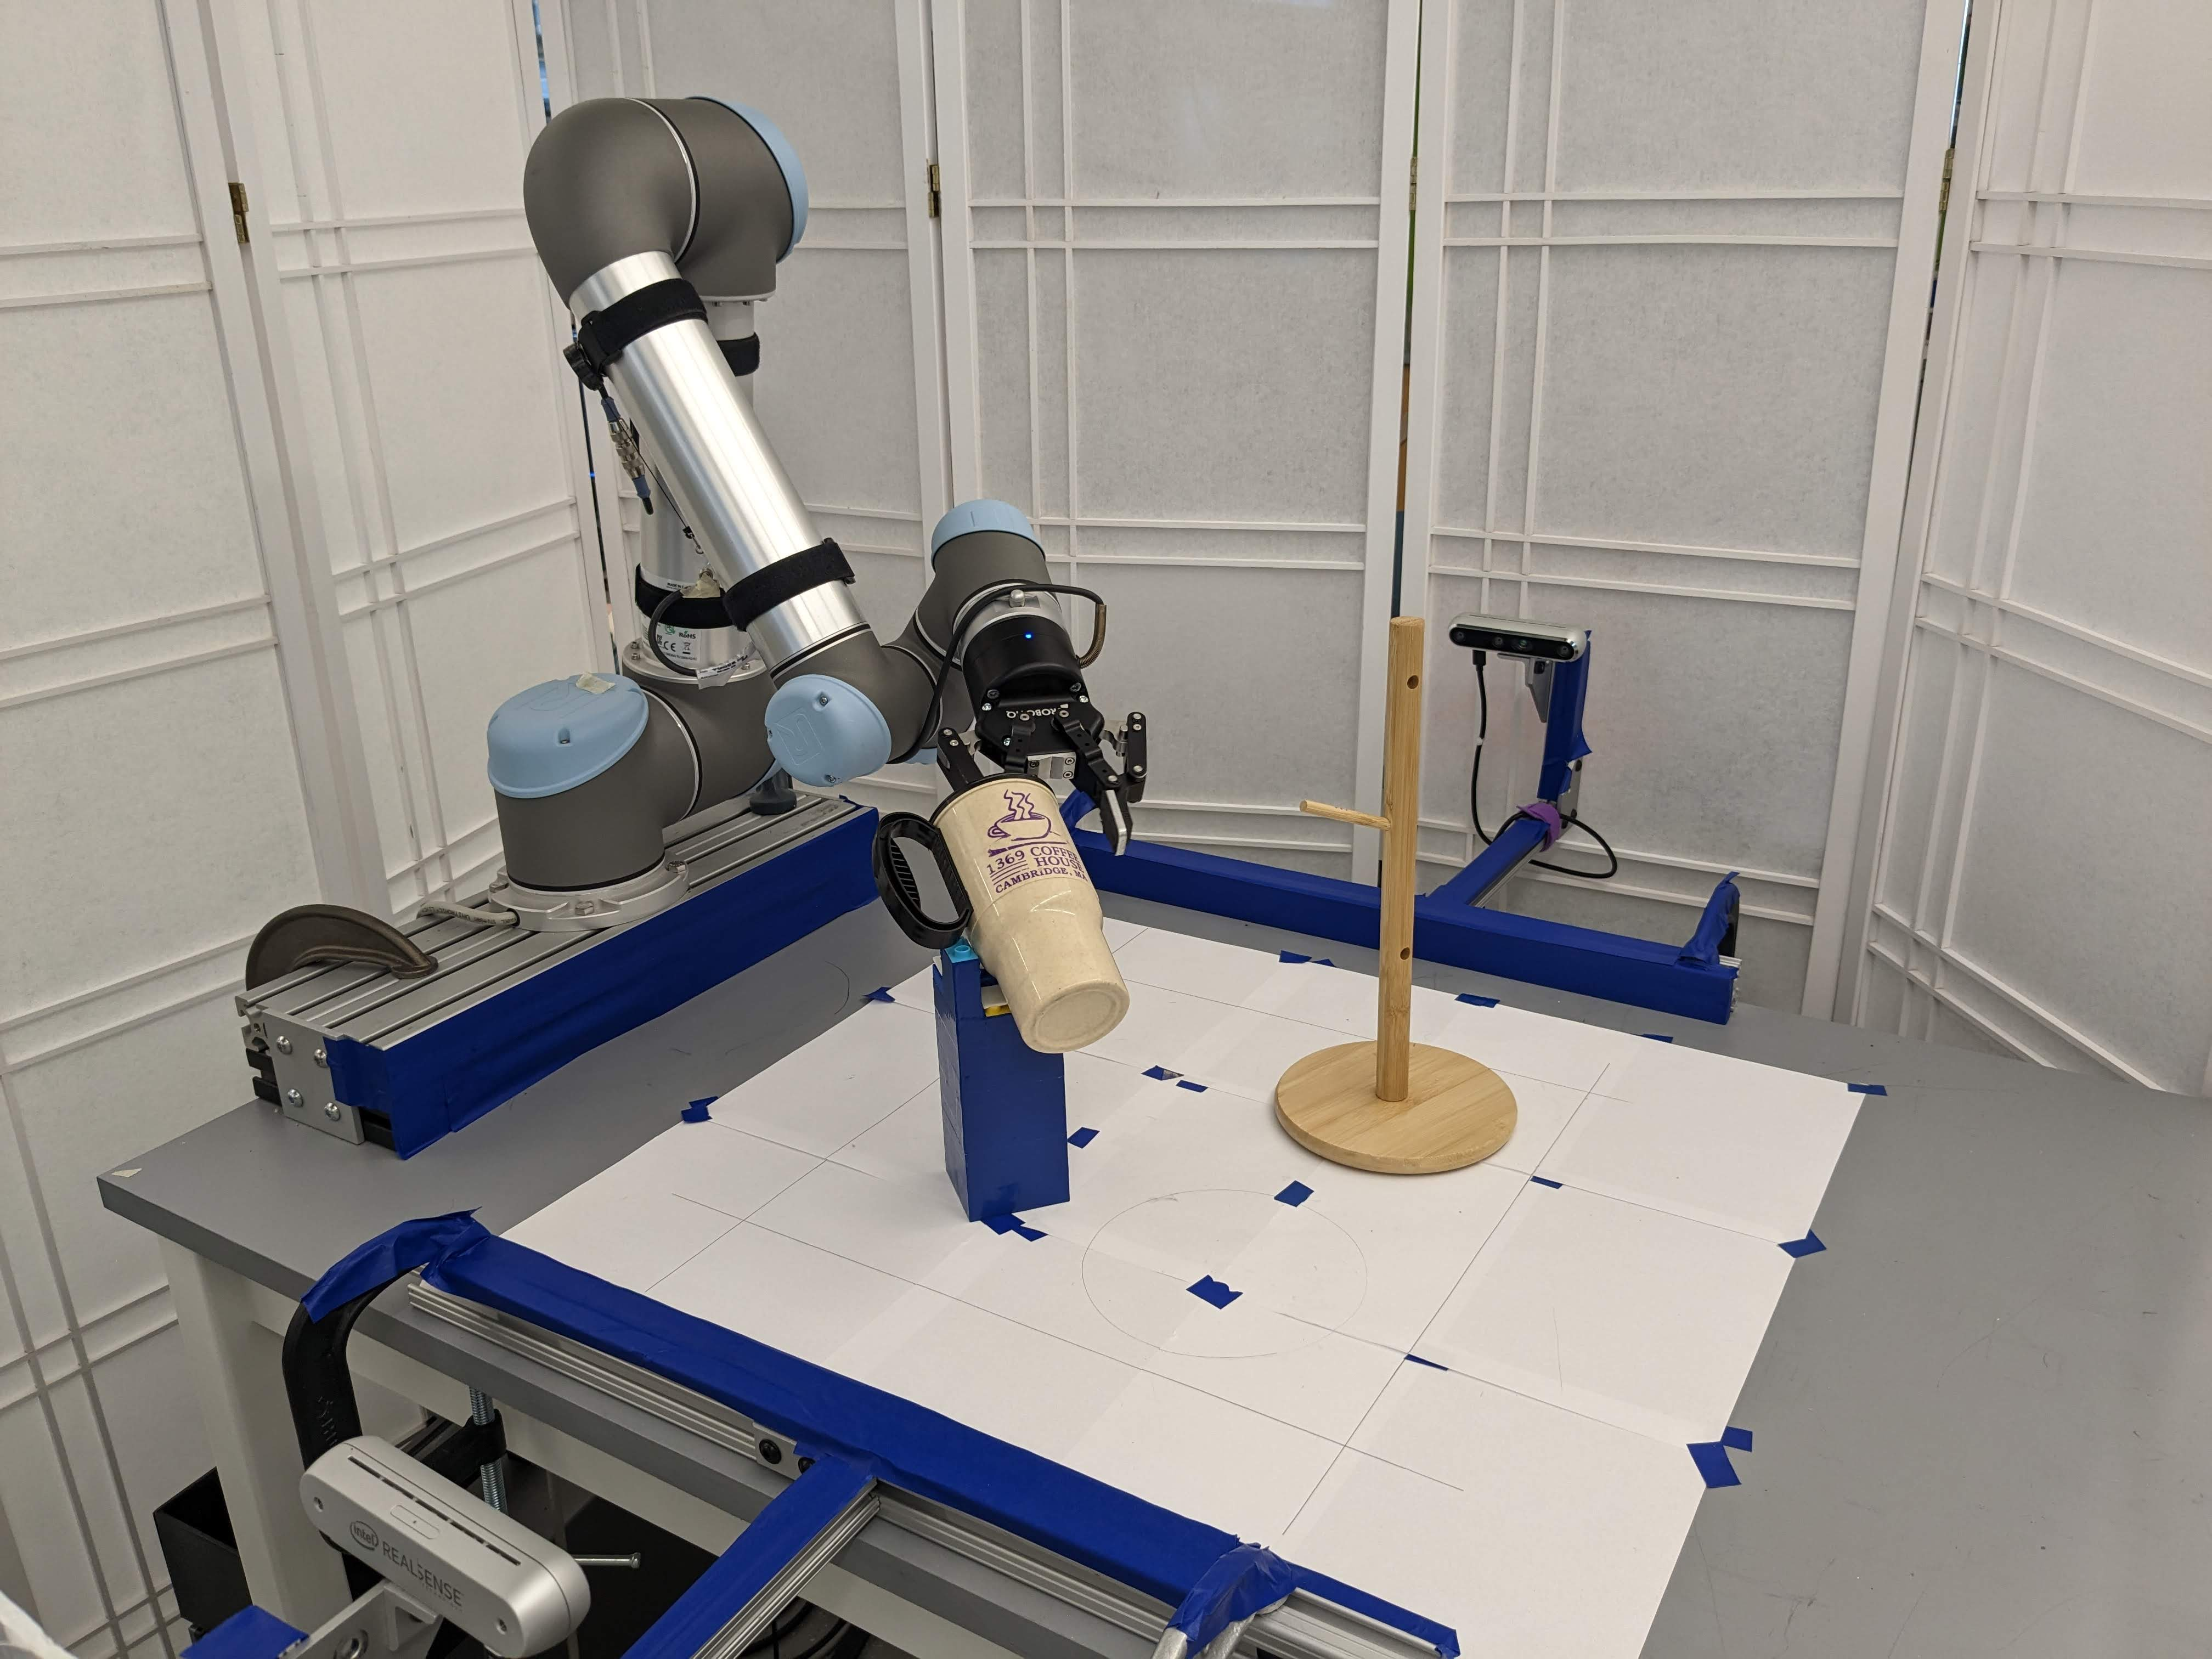
\includegraphics[width=\linewidth]{figures/episodes/mug_on_tree/4.jpg}
    \end{subfigure}
    \begin{subfigure}{(\linewidth - 0.05\linewidth)/5}
        \centering
        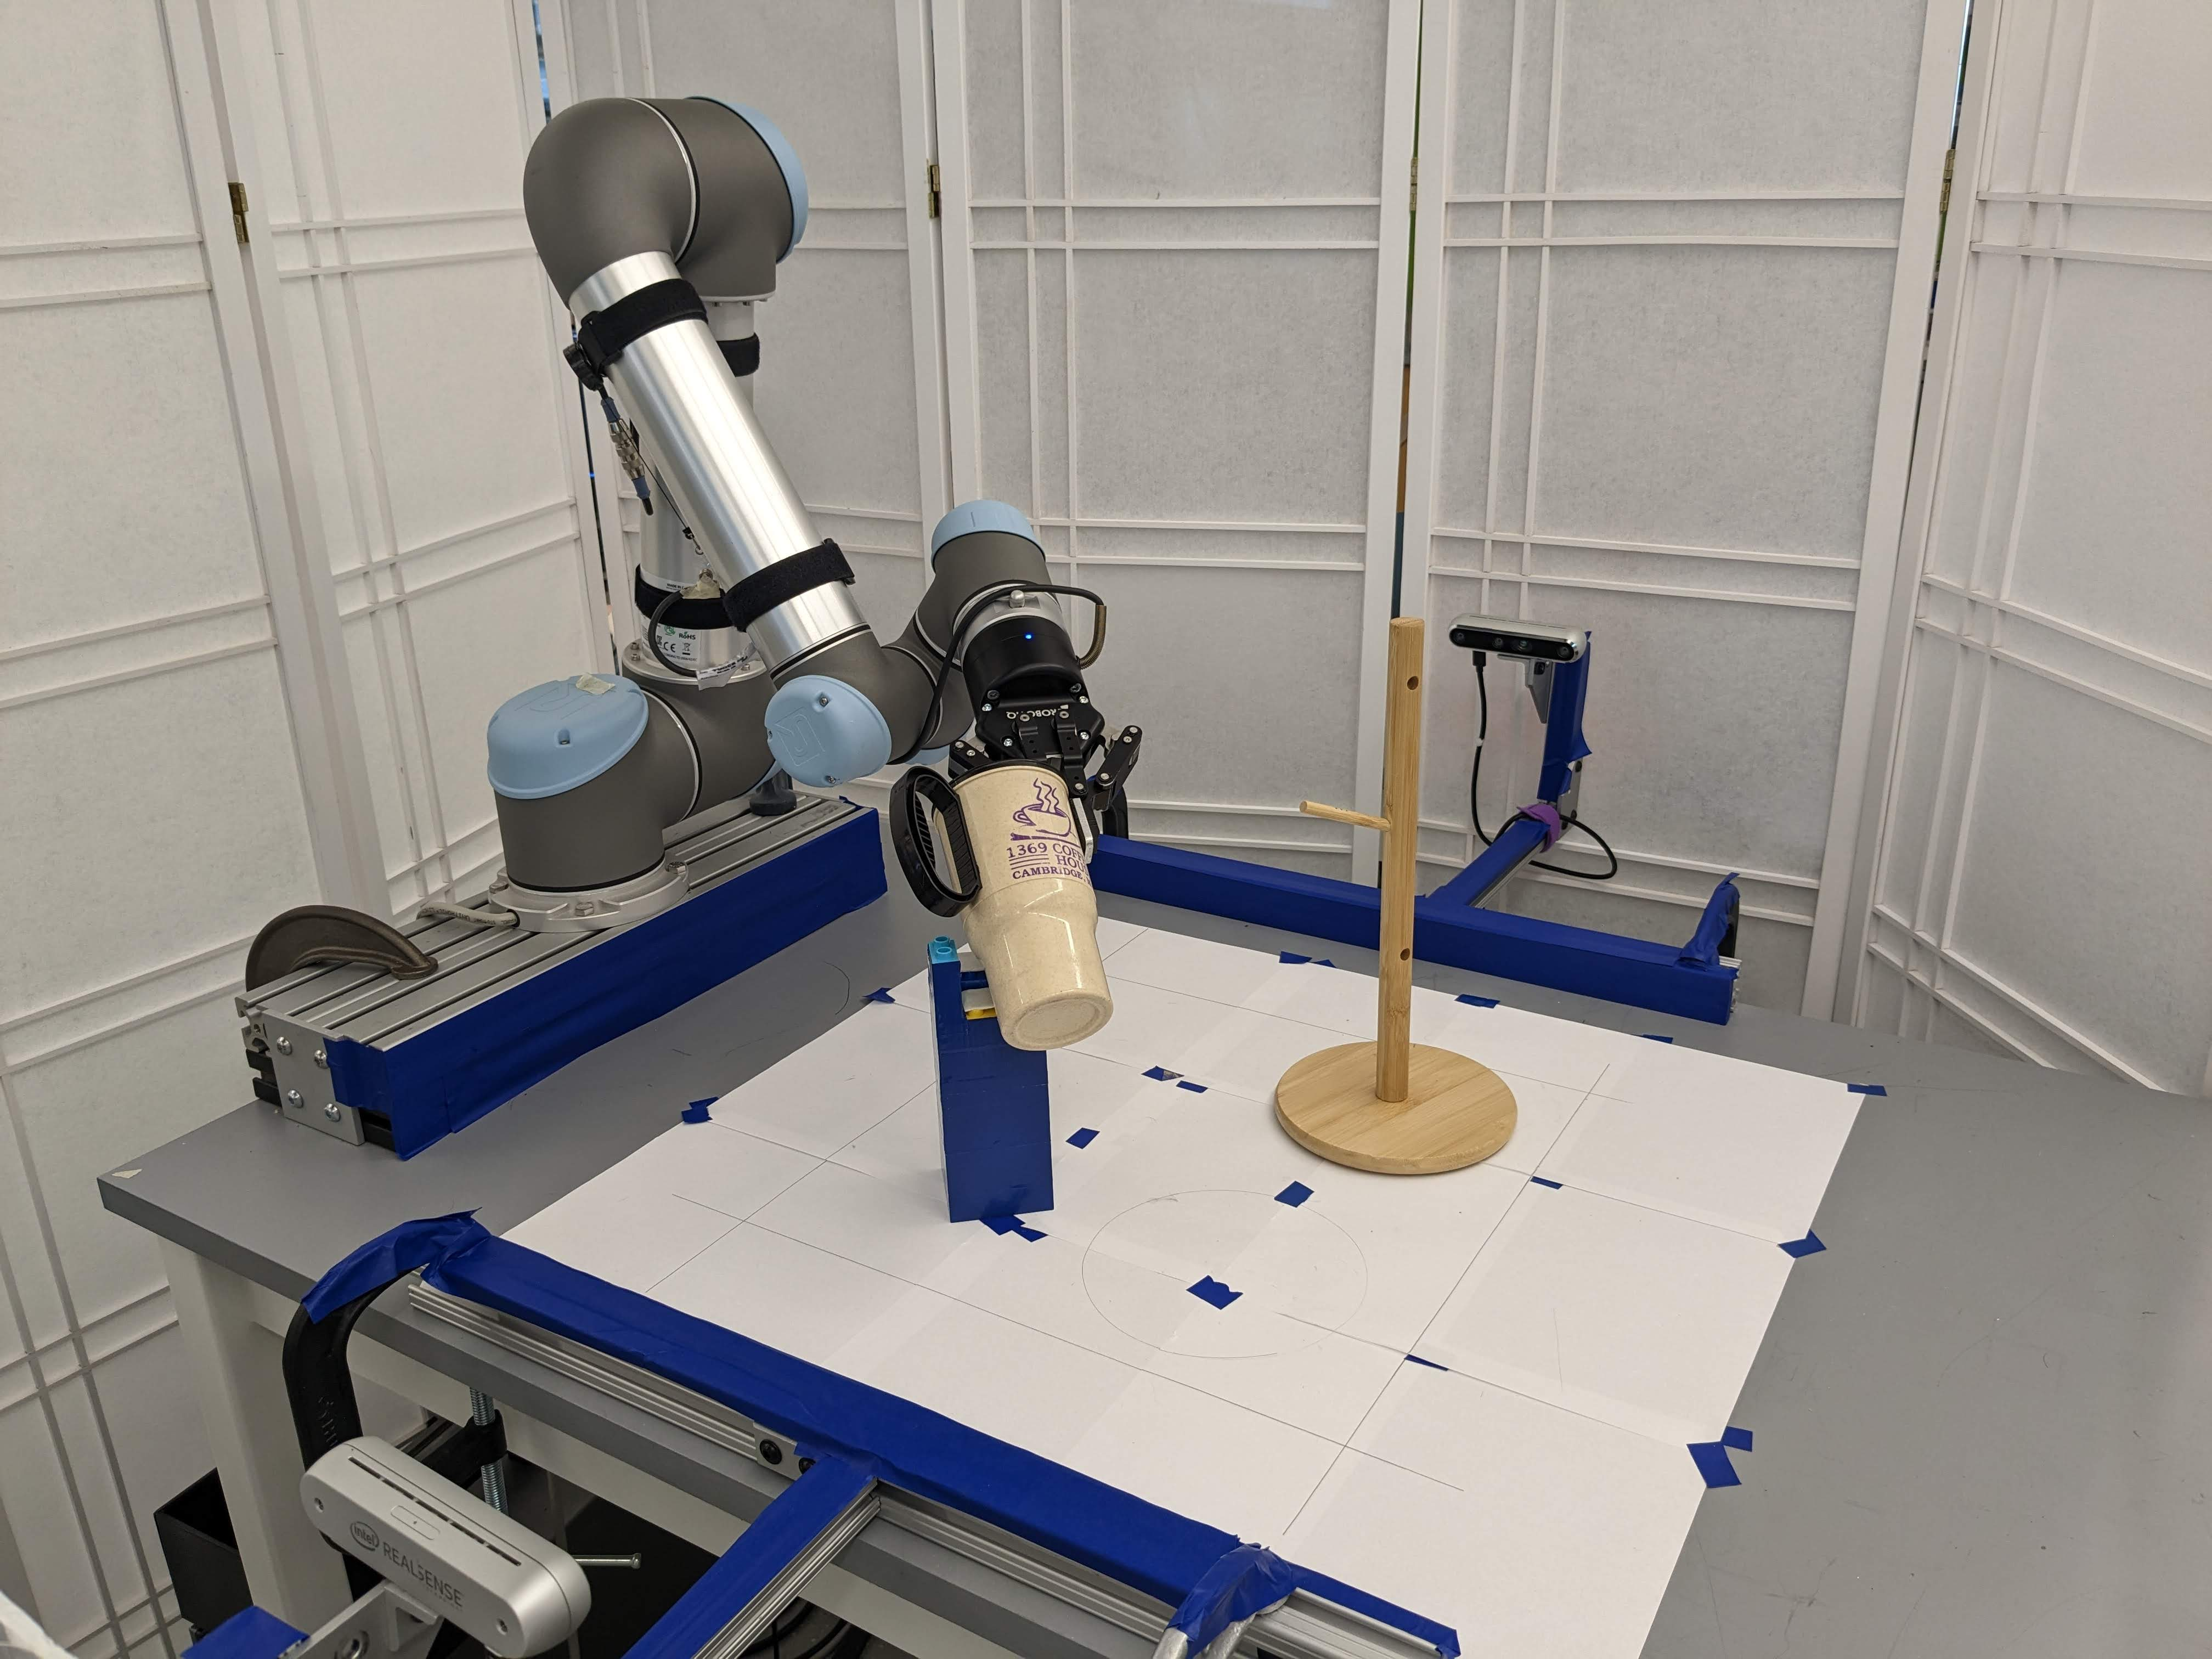
\includegraphics[width=\linewidth]{figures/episodes/mug_on_tree/5.jpg}
    \end{subfigure}
    \begin{subfigure}{(\linewidth - 0.05\linewidth)/5}
        \centering
        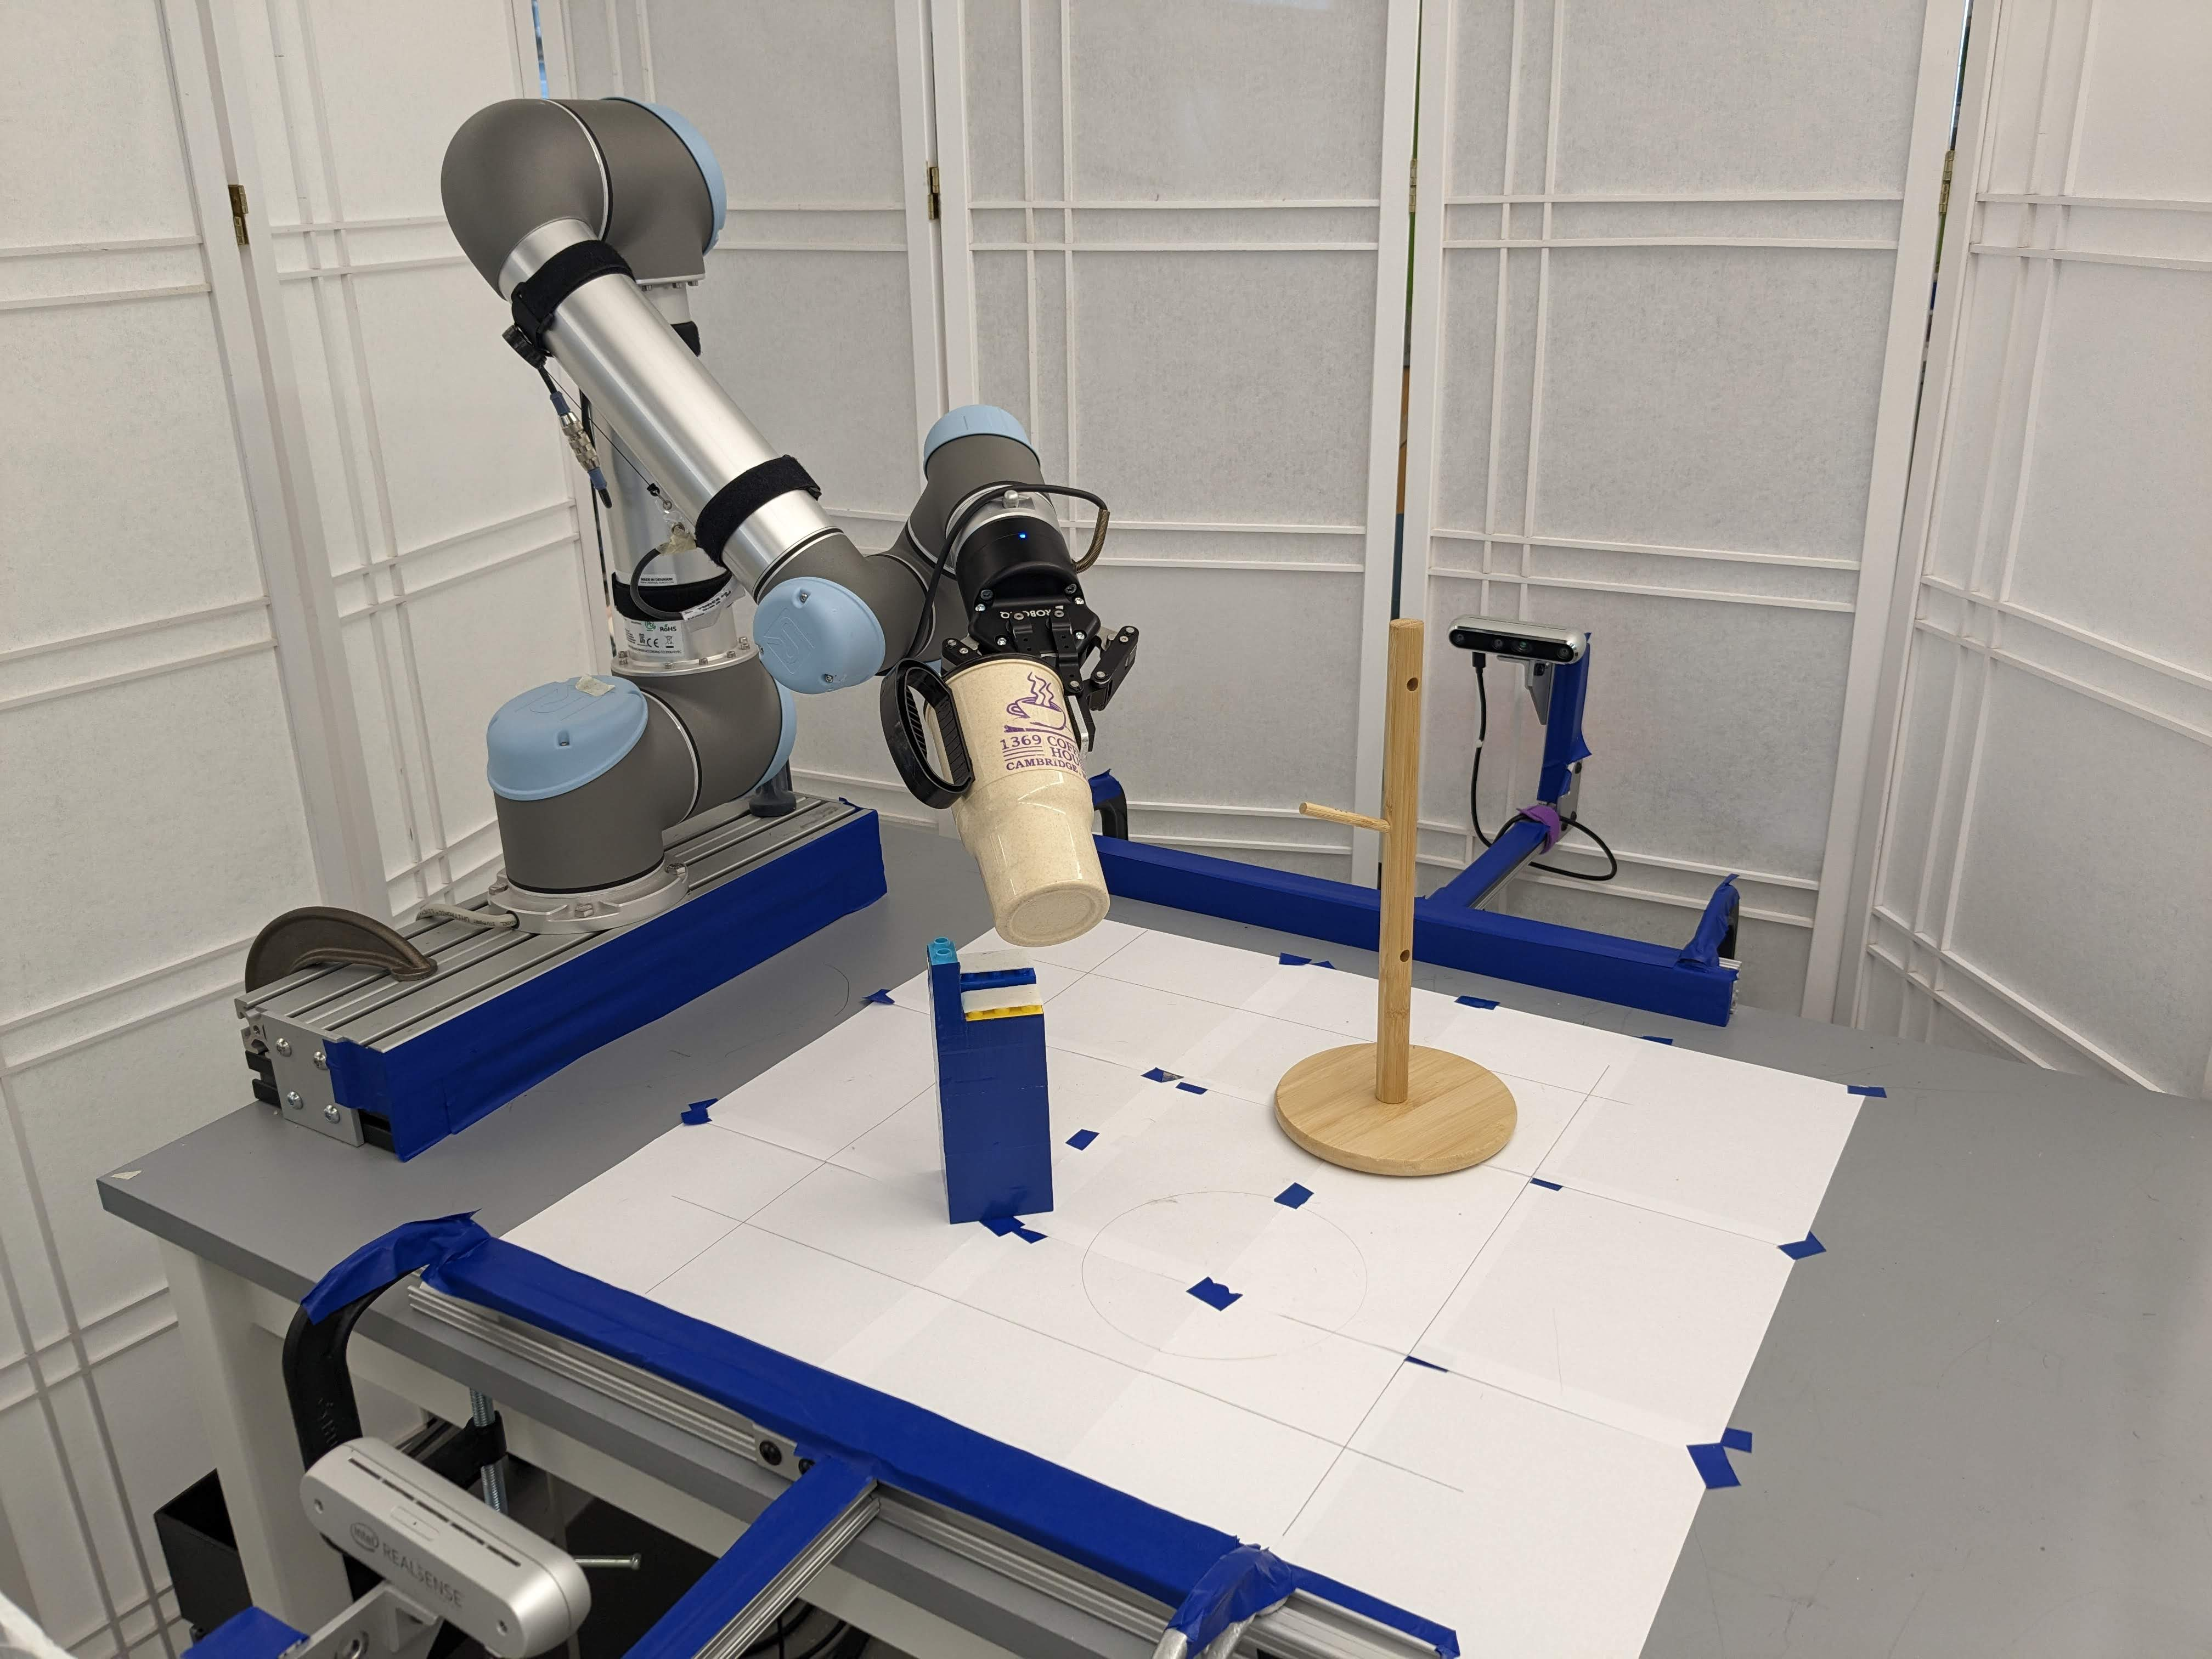
\includegraphics[width=\linewidth]{figures/episodes/mug_on_tree/6.jpg}
    \end{subfigure}
    \begin{subfigure}{(\linewidth - 0.05\linewidth)/5}
        \centering
        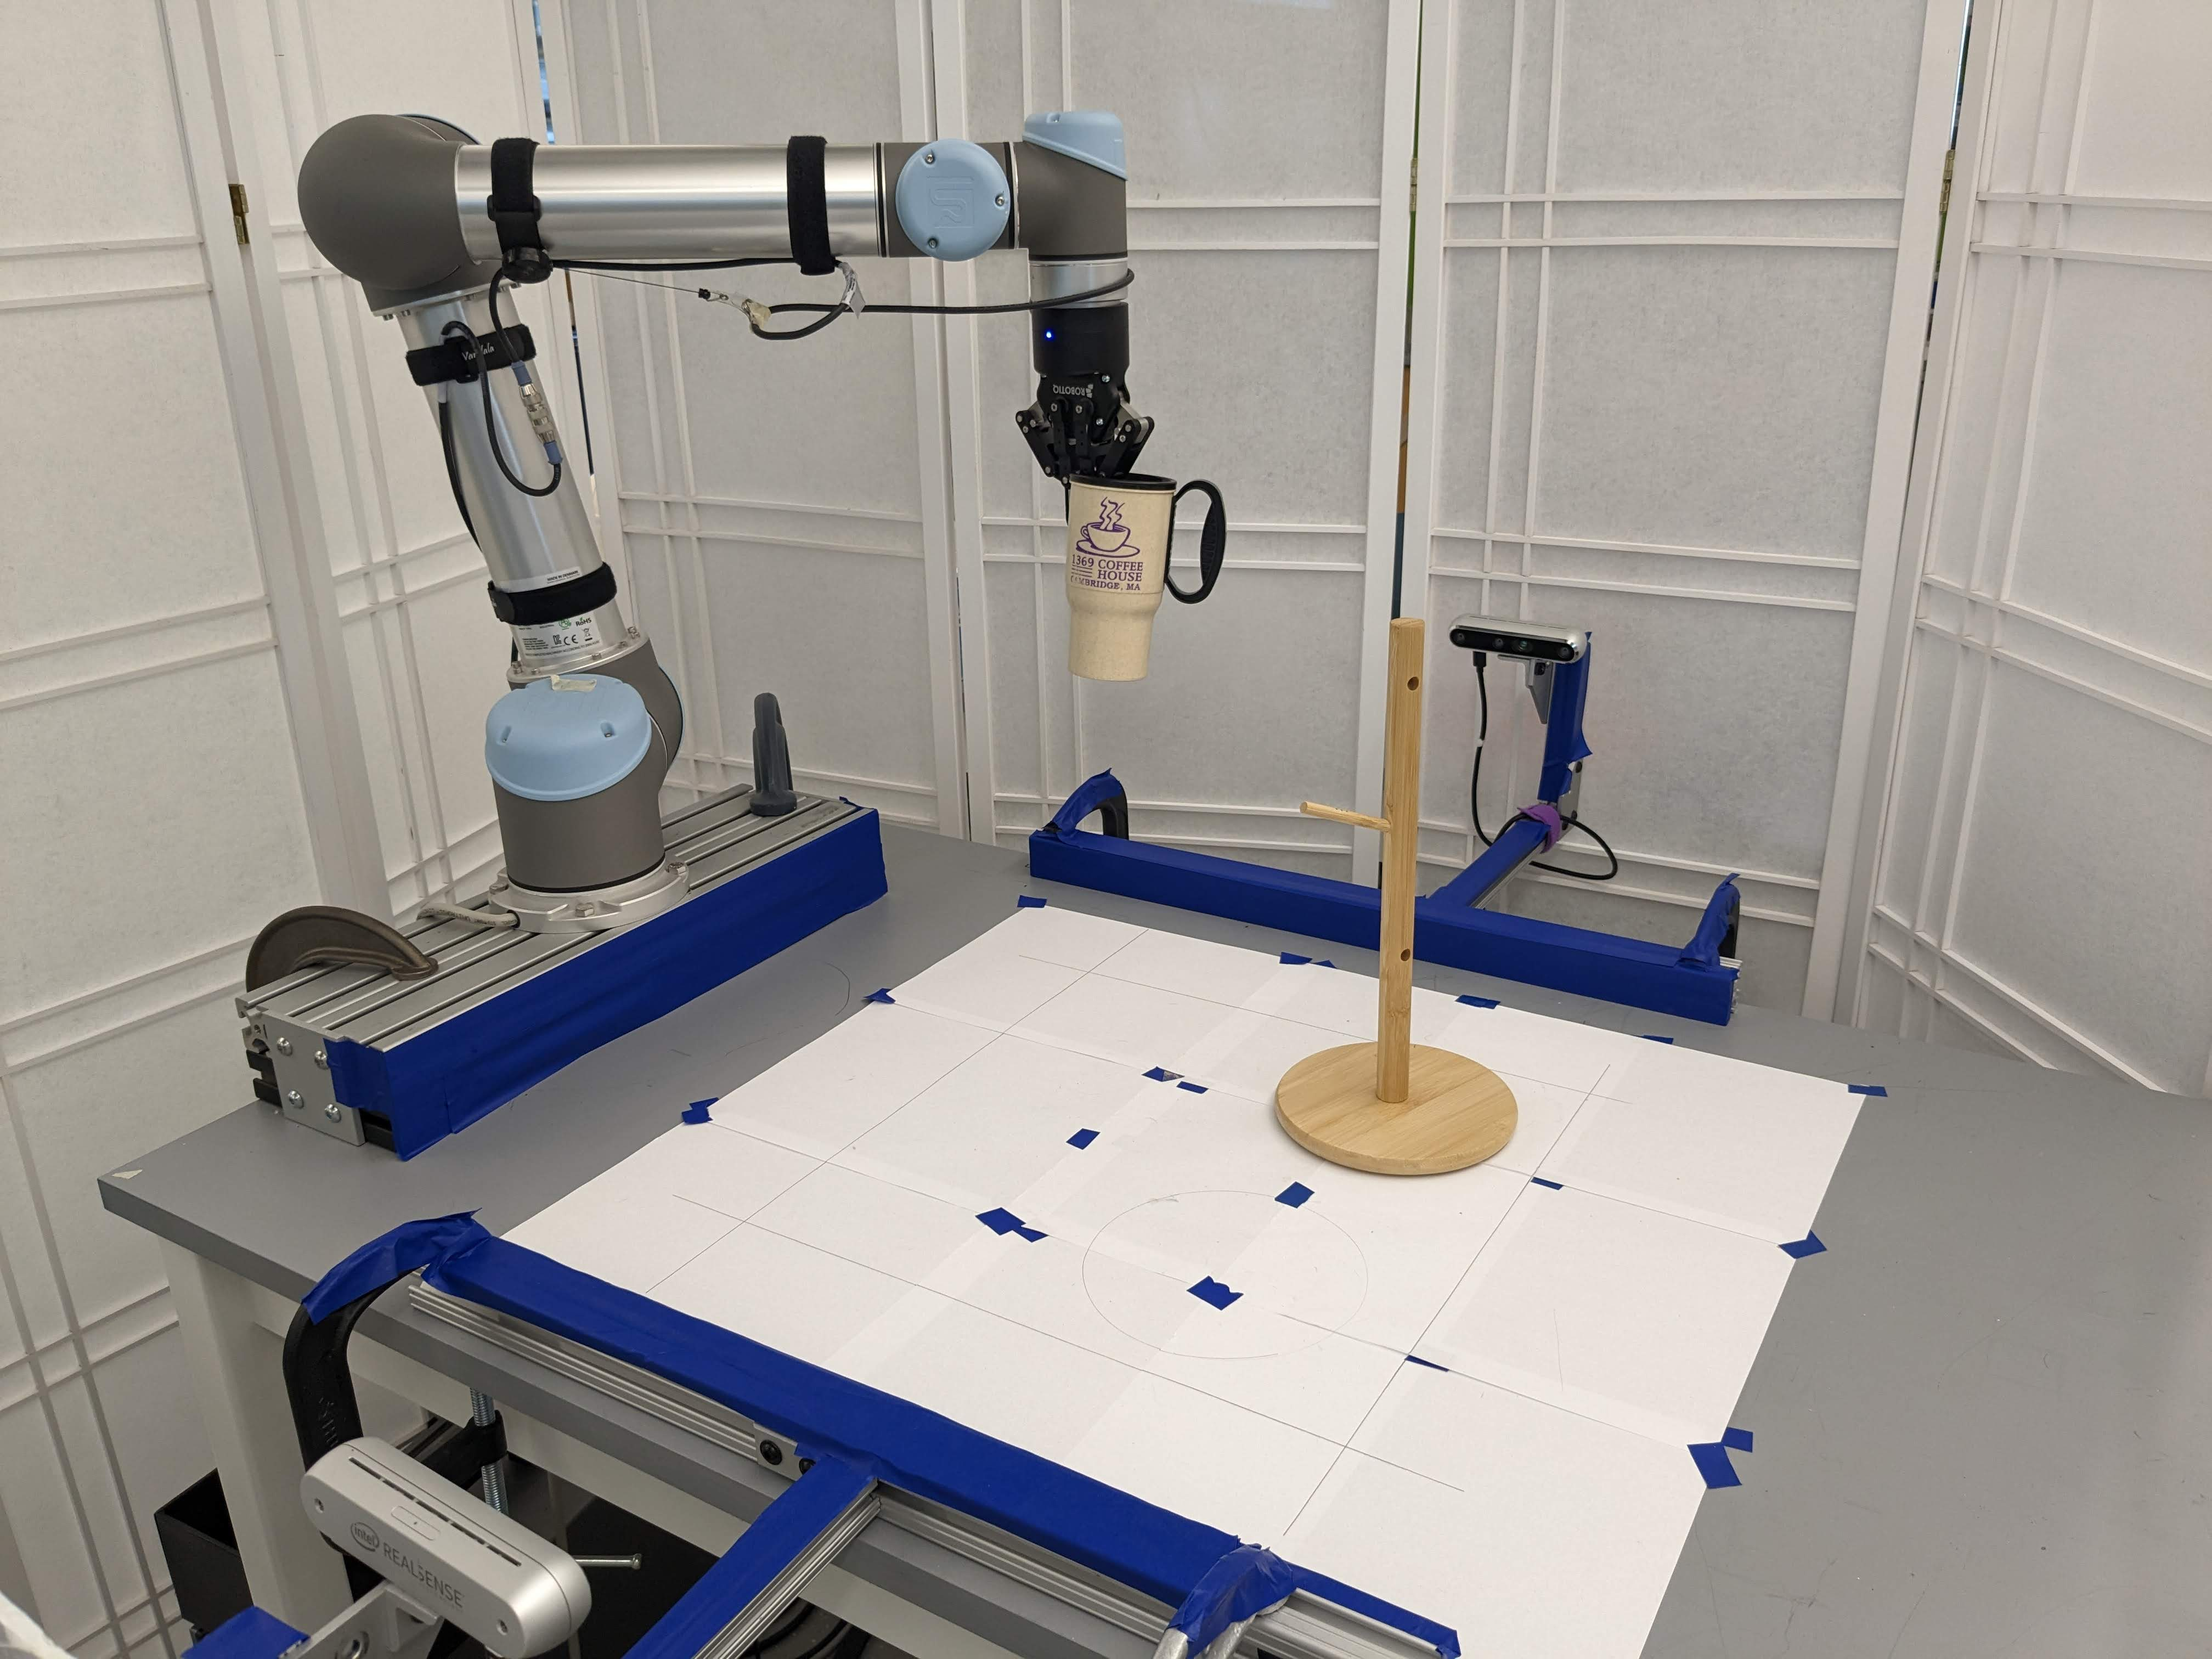
\includegraphics[width=\linewidth]{figures/episodes/mug_on_tree/7.jpg}
    \end{subfigure}
    \begin{subfigure}{(\linewidth - 0.05\linewidth)/5}
        \centering
        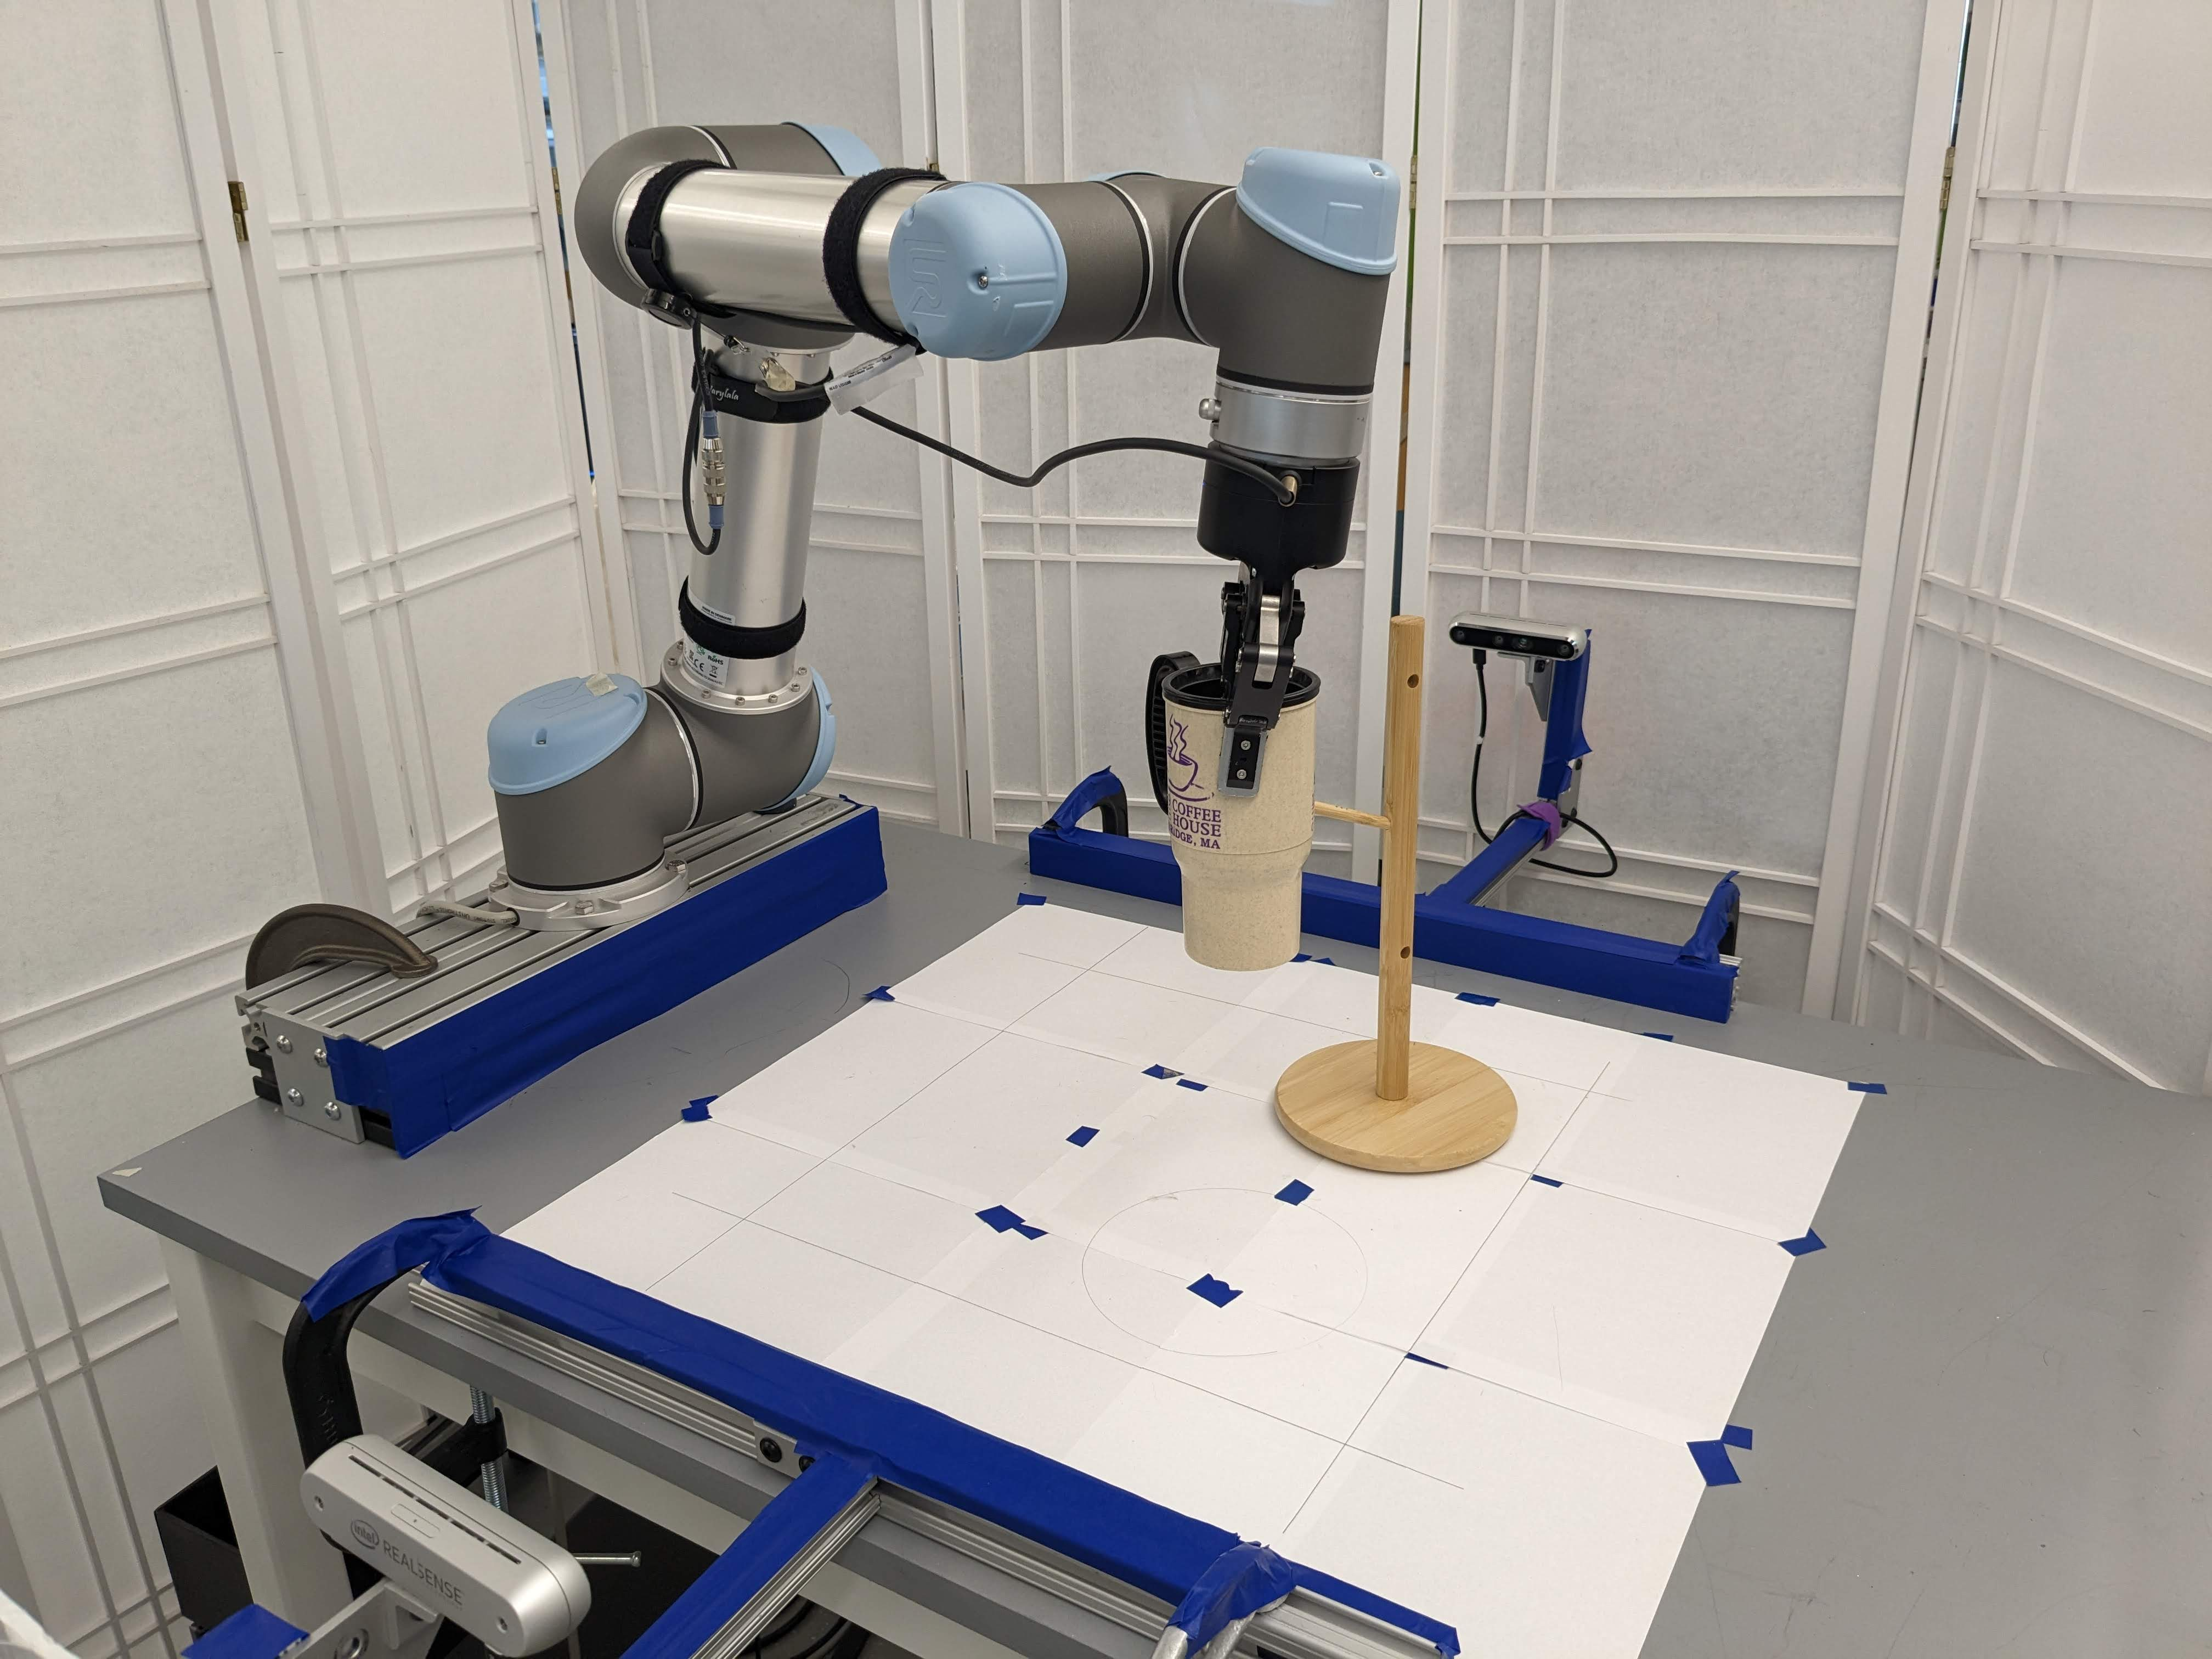
\includegraphics[width=\linewidth]{figures/episodes/mug_on_tree/8.jpg}
    \end{subfigure}
    \begin{subfigure}{(\linewidth - 0.05\linewidth)/5}
        \centering
        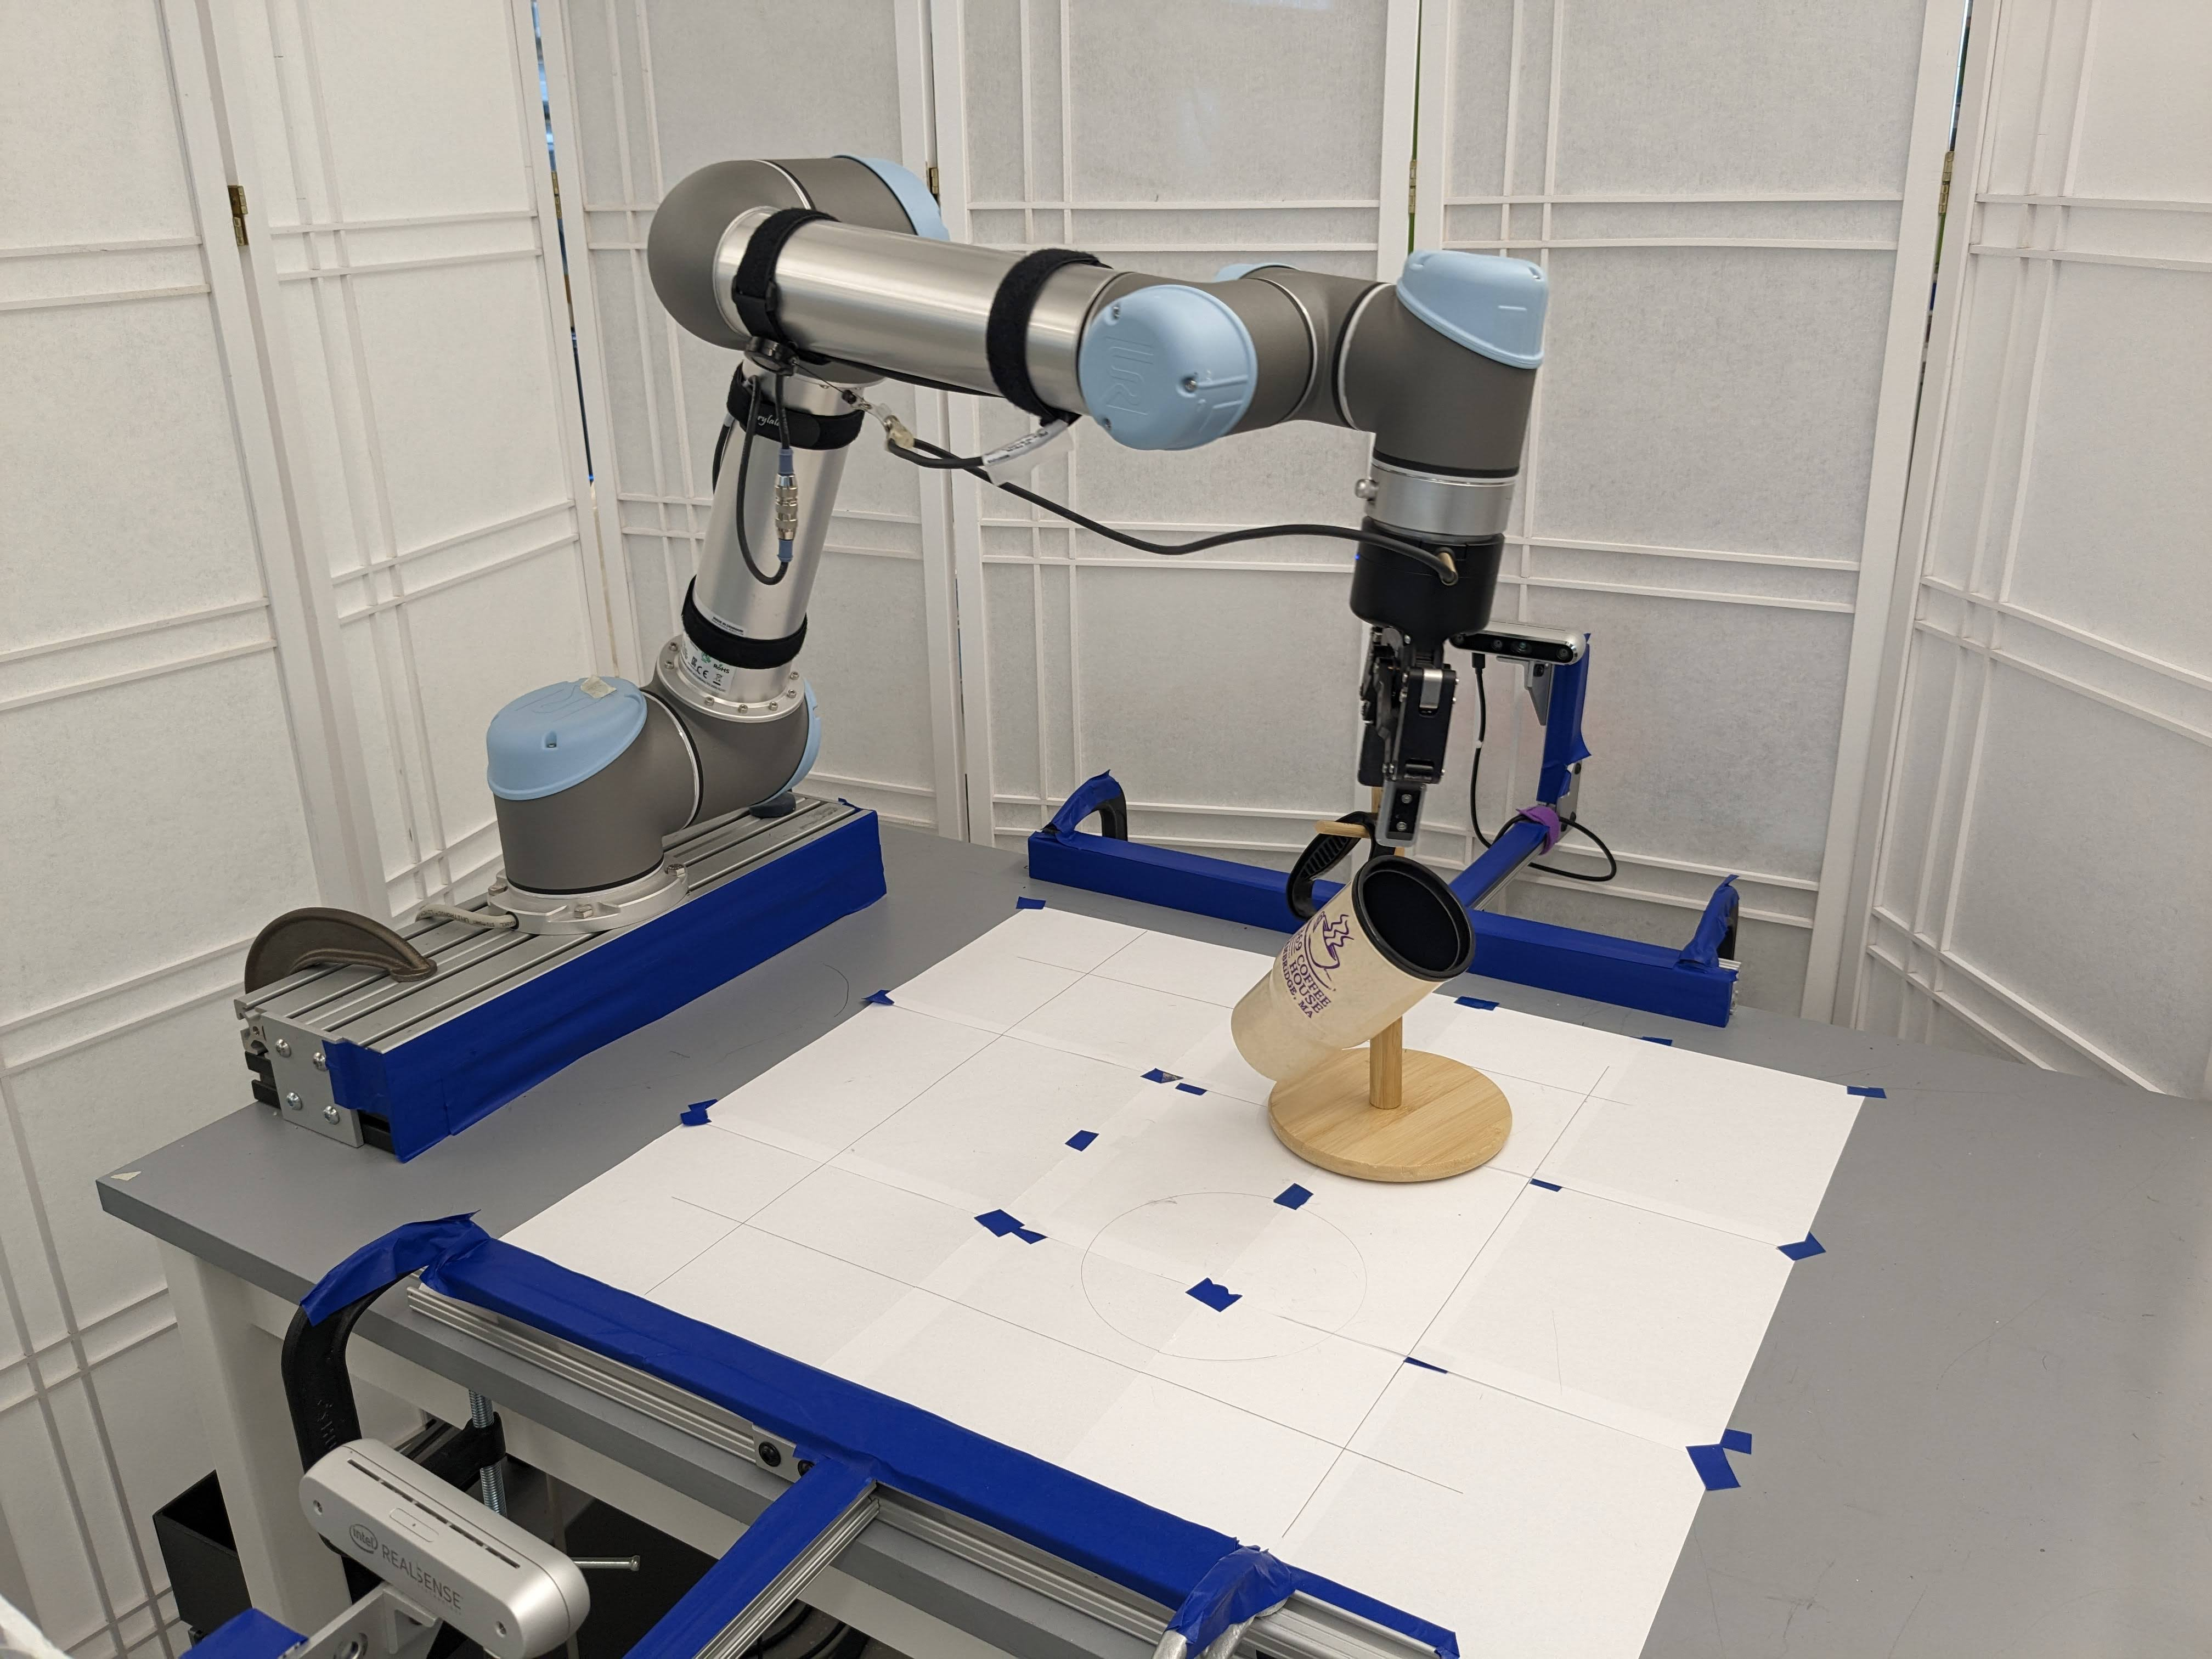
\includegraphics[width=\linewidth]{figures/episodes/mug_on_tree/9.jpg}
    \end{subfigure}
    \begin{subfigure}{(\linewidth - 0.05\linewidth)/5}
        \centering
        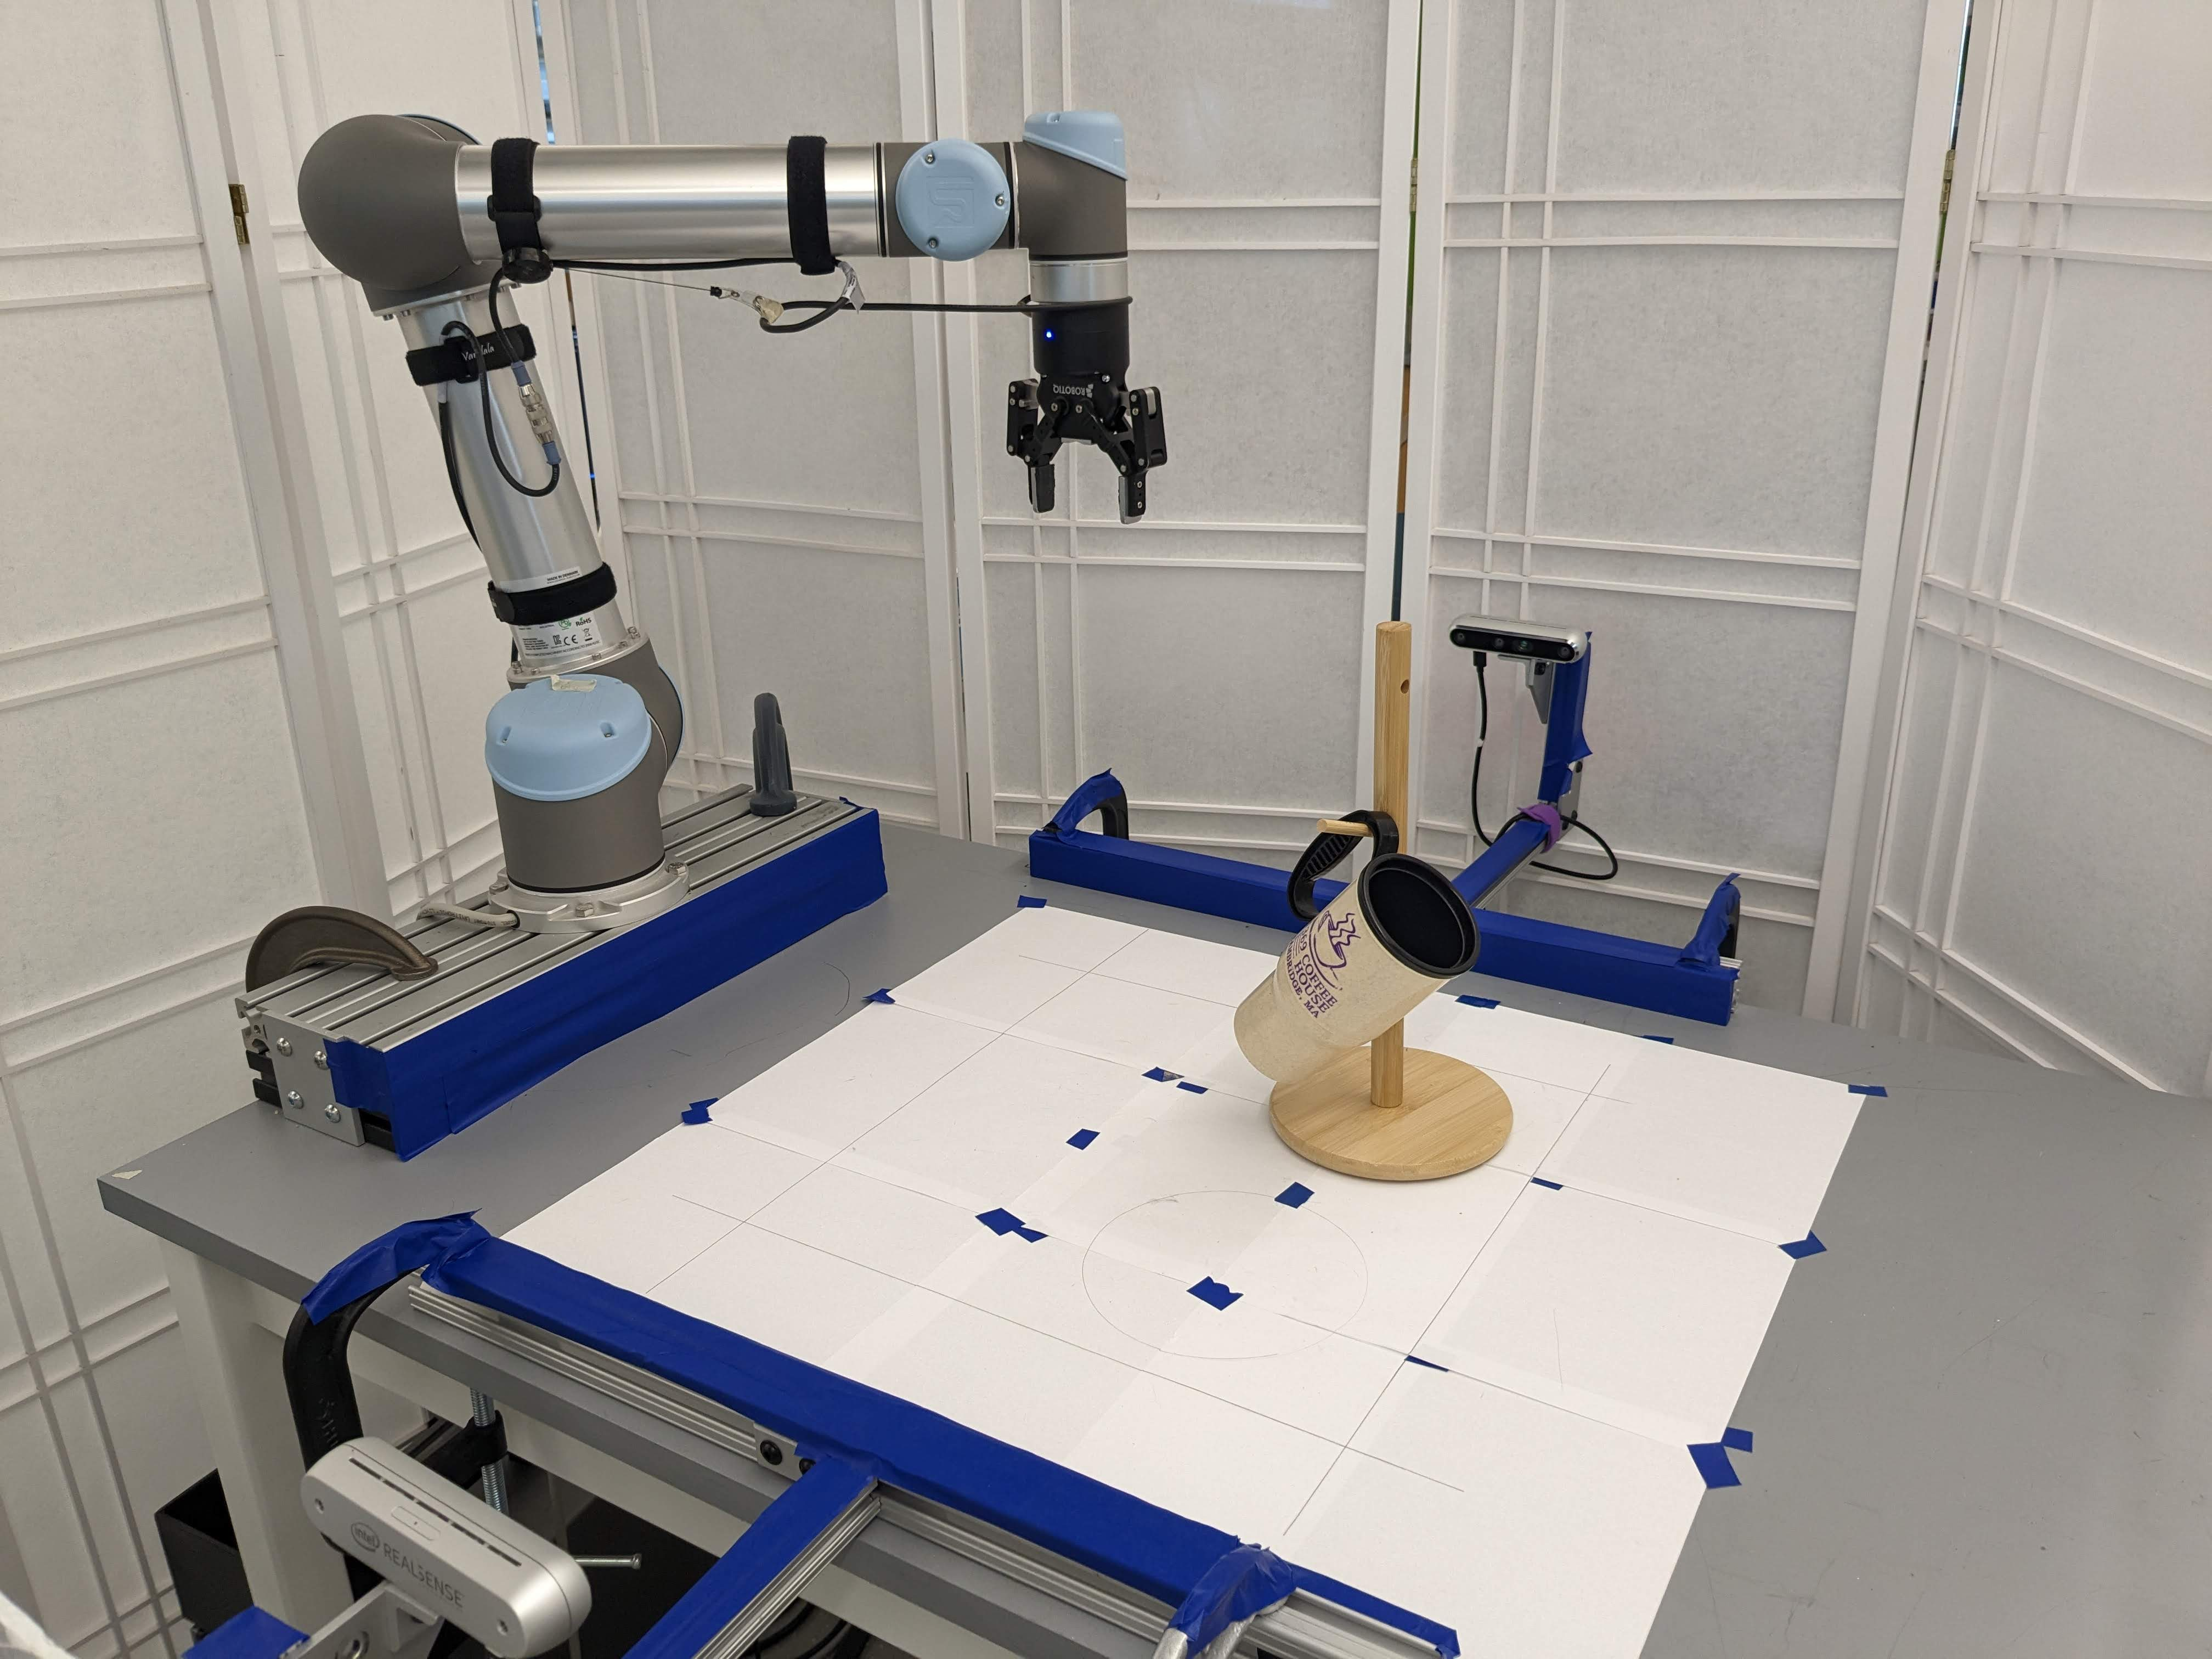
\includegraphics[width=\linewidth]{figures/episodes/mug_on_tree/10.jpg}
    \end{subfigure}

    \caption{Example of an episode of putting a mug on a tree starting from a tilted mug pose.}
    \label{fig:mug_tree_episode}
\end{figure}

\begin{table}[h]
    \centering
    \begin{tabular}{lllcccccc}
        \toprule
          & & \# Train. & \multicolumn{2}{c}{\textbf{Mug on Tree}} & \multicolumn{2}{c}{\textbf{Bowl on Mug}} & \multicolumn{2}{c}{\textbf{Bottle in Container}} \\
         \textbf{Method} & \# Demos & Meshes & Upright & Arbitrary & Upright & Arbitrary & Upright & Arbitrary \\
         \midrule
         R-NDF & 1 & 200 & 60.0 & 51.0 & 69.0 & 68.0 & 19.0 & 8.0 \\
         TAX-Pose & 1 & 200 & 61.0 & 41.0 & 16.0 & 9.0 & - & - \\
         \textbf{IW} & 1 & 10 & \textbf{86.0} & \textbf{83.0} & \textbf{82.0} & \textbf{84.0} & \textbf{62.0} & \textbf{60.0} \\
         \midrule
         R-NDF & 5 & 200 & 88.0 & \textbf{89.0} & 53.0 & 46.0 & 78.0 & 47.0 \\
         TAX-Pose & 5 & 200 & 82.0 & 51.0 & 29.0 & 14.0 & - & - \\
         \textbf{IW} & 5 & 10 & \textbf{90.0} & 87.0 & \textbf{75.0} & \textbf{77.0} & \textbf{79.0} & \textbf{79.0} \\
         \midrule
         R-NDF \cite{simeonov22se} & 10 & 200 & 71.0 & 70.0 & 69.0 & 60.0 & \textbf{81.0} & 59.0 \\
         TAX-Pose \cite{pan22taxpose} & 10 & 200 & 82.0 & 52.0 & 20.0 & 20.0 & 2.0 & 1.0 \\
         \textbf{IW (Ours)} & 10 & 10 & \textbf{88.0} & \textbf{88.0} & \textbf{83.0} & \textbf{86.0} & 70.0 & \textbf{83.0} \\
         \bottomrule
    \end{tabular}
    \caption{Success rates of predicted target poses of objects in \hl{simulation}. Upright and Arbitrary refer to the starting pose of the manipulated object. Each entry is measured over 100 trials with unseen object pairs.}
    \label{tab:simulation}
\end{table}

\begin{table*}[t!]
    \centering
    \begin{tabular}{lcccccc|cc}
         \toprule
          & \multicolumn{2}{c}{\textbf{Mug on Tree}} & \multicolumn{2}{c}{\textbf{Bowl on Mug}} & \multicolumn{2}{c}{\textbf{Bottle in Container}} & \multicolumn{2}{c}{\textbf{Mean}} \\
         \textbf{Method} & Pick & Pick\&Place & Pick & Pick\&Place & Pick & Pick\&Place & Pick & Pick\&Place \\
         \midrule
         NDF$^1$ \cite{simeonov22neural} & 93.3 & 26.7 & 75.0 & 33.3 & 20.0 & 6.7 & 62.8 & 22.2 \\
         R-NDF \cite{simeonov22se} & 60.0 & 13.3 & 41.7 & 41.7 & 33.3 & 20.0 & 45.0 & 25.0 \\
         \textbf{IW (Ours)} & \textbf{100.0} & \textbf{93.3} & \textbf{83.3} & \textbf{75.0} & \textbf{80.0} & \textbf{73.3} & \textbf{87.8} & \textbf{80.5} \\
         \bottomrule
    \end{tabular}
    \caption{Success rates of \hl{real-world robot} pick-and-place experiments with a single demonstration. The manipulated object (e.g. a mug) starts in an arbitrary pose (we use a stand to get a range of poses) and the target object (e.g. a mug-tree) starts in an arbitrary upright pose. $^1$The target object (e.g. the mug tree) is in a fixed pose for this experiment, as NDF does not handle target object variation. Each entry is measured over 25 - 30 trials with unseen object pairs.}
    \label{tab:real_world}
\end{table*}

\textbf{Setup:} For our simulated experiment, we use an open-source environment with three tasks: mug on a mug-tree, bowl on a mug and a bottle in a  container \cite{simeonov22se}\footnote{\url{https://github.com/anthonysimeonov/relational_ndf}}. Given a segmented point cloud of the initial scene, the goal is to predict the pose of the child object relative to the parent object (e.g.~the mug relative to the mug-tree) so that the task constraint is satisfied. The simulation does not test grasp prediction.

For our real-world experiment, we perform both grasps and placements based on a single demonstration. We capture a fused point cloud using three RealSense D455 depth cameras. We use point cloud clustering and heuristics to detect objects in the real-world scenes (details in Appendix \ref{appendix:experiment:rearrangement}) and perform motion planning with collision checking based on the meshes predicted by our method. We evaluate the ability of each method to pick and place unseen objects with a varying shape and pose (Figure \ref{fig:object_sets}).

\textbf{Result:} We find that interaction warping generally outperforms Relational Neural Descriptor Fields \cite{simeonov2022neural} and TAX-Pose \cite{pan22taxpose} on the simulated relational placement prediction tasks (Table \ref{tab:simulation}) with 20 times fewer training objects. IW can succeed with one demonstration of a task, whereas R-NDF and TAX-Pose usually require five demonstrations. 

In real-world pick and place experiments, we demonstrate the ability of IW to solve the three object re-arrangement tasks -- mug on tree, bowl on mug and bottle in box -- with unseen objects and variation in the starting pose of objects (Table \ref{tab:real_world}). We find that (Relational) Neural Descriptor Fields \cite{simeonov22neural,simeonov22se} struggle with the partial and noisy real-world point clouds. This often results in both the pick and place actions being too imprecise to successfully solve the task. Pre-training (R-)NDF on real-world point clouds could help, but note that IW was also pre-trained on simulated point clouds. We find that the warping of canonical objects is more robust to noisy and occluded point clouds. We show an example episode of mug on tree in Figure \ref{fig:mug_tree_episode}.

We used the meshes predicted by IW to perform collision checking during motion planning. We do not perform collision checking (other than to avoid contact with the table) when using (R-)NDF as these methods do not predict object meshes, but failures due to a collision between the robot and one of the object were infrequent.

% \subsection{Trajectory Cloning}
% \label{sec:exp:trajectory}
% \textbf{Setup:} We record a single demonstration of a robot painting a particular pattern on a canvas with a brush. We then automatically segment this demonstration into waypoints and record the contact of the brush with the canvas at various waypoints. During testing, the robot uses a different brush and paints on a canvas that is potentially curved. We show that we can make predictions about the object poses that constitute the trajectory regardless of the shape of the brush and the canvas.
% \textbf{Result:} \ob{Abhinav}

\subsection{Grasp Prediction in the Wild}
\label{sec:exp:wild}

\begin{figure}[]
    \centering

    \begin{subfigure}{(\linewidth - 0.05\linewidth)/5}
        \centering
        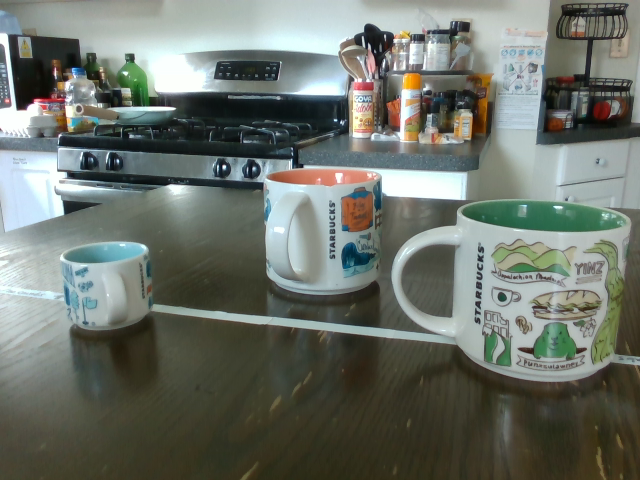
\includegraphics[width=\linewidth]{figures/real2sim2real/2/1.png}
    \end{subfigure}
    \begin{subfigure}{(\linewidth - 0.05\linewidth)/5}
        \centering
        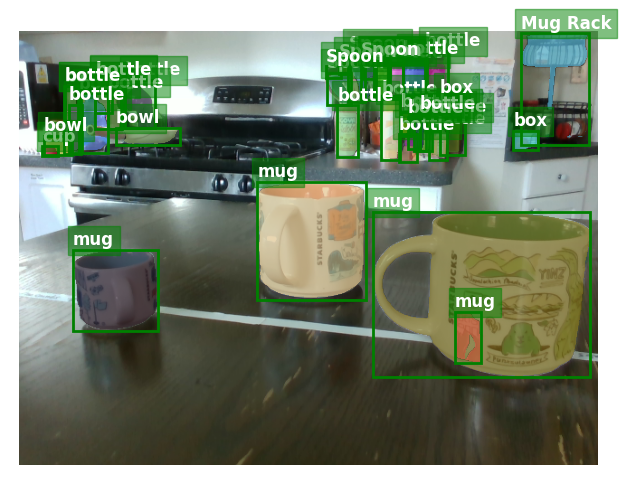
\includegraphics[width=\linewidth]{figures/real2sim2real/2/0.png}
    \end{subfigure}
    \begin{subfigure}{(\linewidth - 0.05\linewidth)/5}
        \centering
        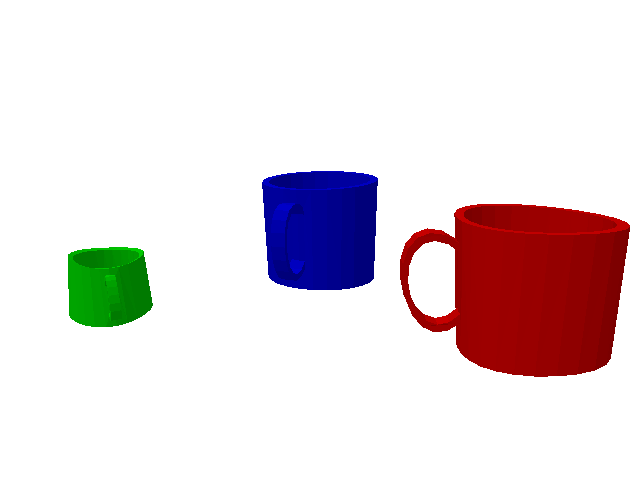
\includegraphics[width=\linewidth]{figures/real2sim2real/2/3_sim.png}
    \end{subfigure}
    \begin{subfigure}{(\linewidth - 0.05\linewidth)/5}
        \centering
        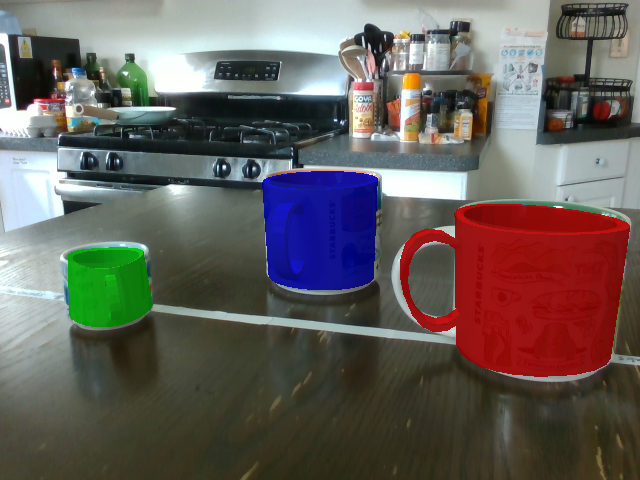
\includegraphics[width=\linewidth]{figures/real2sim2real/2/3.png}
    \end{subfigure}
    \begin{subfigure}{(\linewidth - 0.05\linewidth)/5}
        \centering
        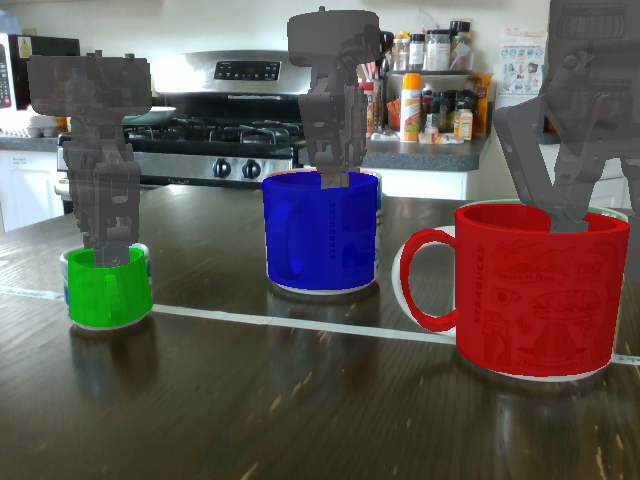
\includegraphics[width=\linewidth]{figures/real2sim2real/2/4.png}
    \end{subfigure}

    \begin{subfigure}{(\linewidth - 0.05\linewidth)/5}
        \centering
        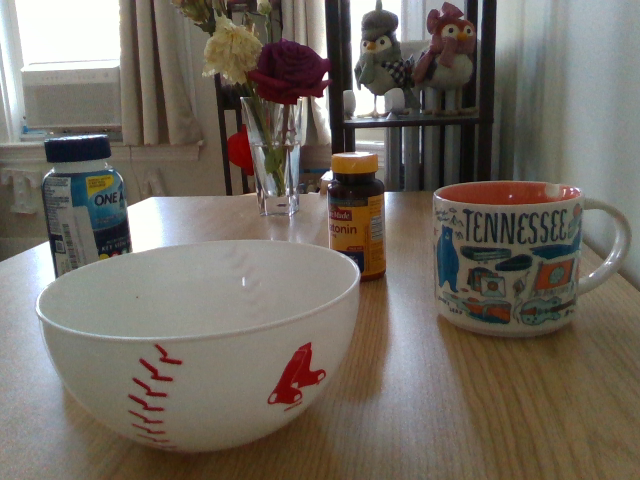
\includegraphics[width=\linewidth]{figures/real2sim2real/5/1.png}
        \caption{}
    \end{subfigure}
    \begin{subfigure}{(\linewidth - 0.05\linewidth)/5}
        \centering
        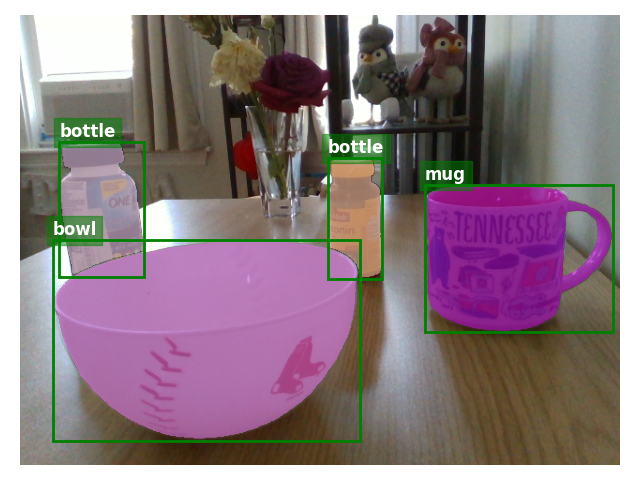
\includegraphics[width=\linewidth]{figures/real2sim2real/5/0.png}
        \caption{}
    \end{subfigure}
    \begin{subfigure}{(\linewidth - 0.05\linewidth)/5}
        \centering
        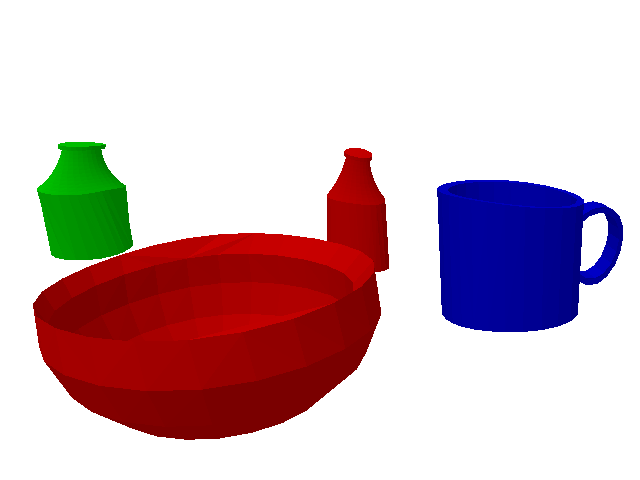
\includegraphics[width=\linewidth]{figures/real2sim2real/5/3_sim.png}
        \caption{}
    \end{subfigure}
    \begin{subfigure}{(\linewidth - 0.05\linewidth)/5}
        \centering
        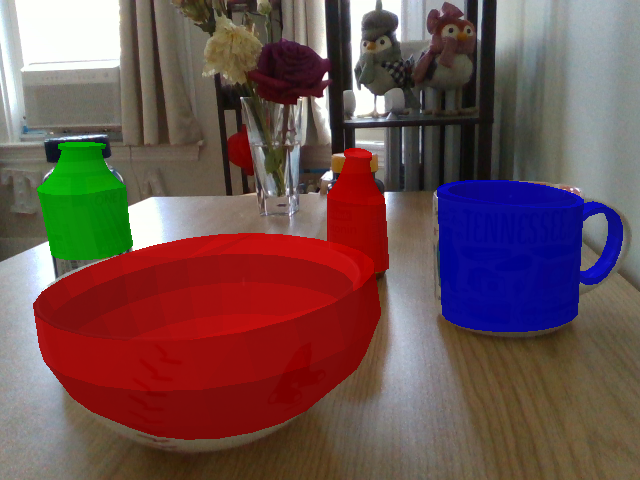
\includegraphics[width=\linewidth]{figures/real2sim2real/5/3.png}
        \caption{}
    \end{subfigure}
    \begin{subfigure}{(\linewidth - 0.05\linewidth)/5}
        \centering
        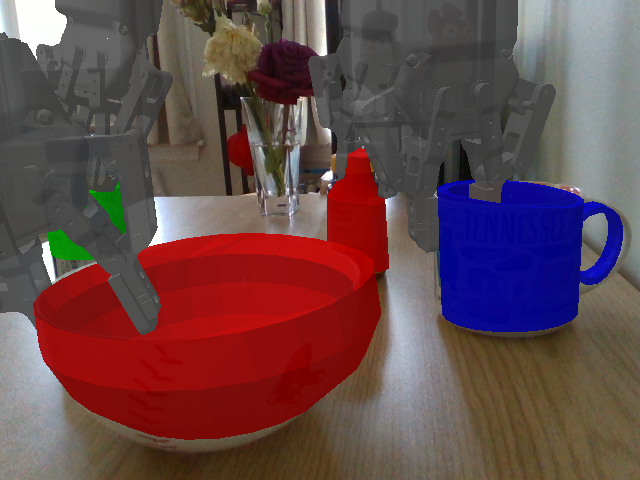
\includegraphics[width=\linewidth]{figures/real2sim2real/5/4.png}
        \caption{}
    \end{subfigure}

    \caption{Grasp prediction in the wild: (a) an RGB-D (depth not shown) image from a RealSense D435 camera, (b) open-vocabulary object detection and segmentation using Detic \cite{zhou22detecting} and Segment Anything \cite{kirillov23segment}, (c) object meshes predicted by our method based on segmented point clouds (we filter out distant and small objects), (d) meshes projected into the original image, (e) grasps predicted by interaction warping projected into the original image. Figure \ref{fig:real2sim2real_part2} has additional examples.}
    \label{fig:real2sim2real}
\end{figure}

\textbf{Setup:} In this experiment, we show that we can combine our method with a state-of-the-art object detection and segmentation pipeline to predict object meshes and robot grasps from a single RGB-D image. We use an open-vocabulary object detector Detic \cite{zhou22detecting} to predict bounding boxes for common household objects and Segment Anything \cite{kirillov23segment} to predict segmentation masks within these bounding boxes. We turn the predicted RGB-D images into point clouds and use our shape warping model to predict a mesh for each object. Finally, we use interaction warping to predict a robot grasp based on a single demonstration per each object class (detailes in Appendix \ref{appendix:experiment:wild}).

\textbf{Result:} We show the results for two example scenes in Figure \ref{fig:real2sim2real} and \ref{fig:real2sim2real_part2}. Our perception pipeline can successfully detect objects in images with cluttered backgrounds. Our warping algorithm accounts for the variation in the shape and size of objects and our interaction warping algorithm can generalize the demonstrated grasps to the novel objects.

\section{Limitations}

\begin{itemize}
    \item We run joint shape warping and pose estimation using gradient descent and many random restarts. This process takes around 25 seconds per object on a single desktop GPU. Future work could train an additional neural network to skip the gradient descent, or to predict favorable initialization.
    \item Shape warping represented using PCA cannot capture the detail of each object. Tasks that require a high-degree of precision might have a low success rate. But, PCA can be easily replaced with a higher capacity model (which might require more than 10 training meshes per object class).
    \item Our method does not learn from its failures; its behavior is fully determined by the shape warping model and a single demonstration. But, the entire prediction process, from shape warping to interaction point cloning, is technically fully differentiable.
    \item While relatively robust to partial and noisy point clouds, our method cannot reason about object parts that are not shown in the point cloud. For example, our method currently cannot infer that a handle of a mug is occluded by the mug itself if it is not shown in the point cloud. It would instead predict an arbitrary orientation of the mug.
\end{itemize}

\section{Conclusion}

We introduced Interaction Warping, a method for one-shot learning of 3D robotic manipulation policies. We have shown that warping of shapes and interaction points leads to successful learning of policies for object re-arrangement. We have also shown that we can use open-vocabulary detection and segmentation models to detect objects in the wild and predict their meshes and possible robot grasps. Future work could equip interaction warping with a more expressive shape warping model, so that it can predict 3D meshes of novel objects with high precision. Another interesting direction is to combine shape warping with object decomposition \cite{tenorth13decomposing,vahrenkamp16partbased,chen22neural} to learn representations of parts of complex objects, such as the door of a toaster oven or a water tank of a coffee machine. Shape warping could be used to represent articulate as well as deformable objects.

%===============================================================================

\clearpage

%===============================================================================

% no \bibliographystyle is required, since the corl style is automatically used.
\bibliography{main,zotero,references-rob}  % .bib

\clearpage
\appendix

\section{Method Details}
\label{appendix:method}

\begin{algorithm}[H]

\caption{Warp Learning}\label{alg:warp_learn} 

\begin{flushleft}
    \hspace*{\algorithmicindent} \textbf{Input:} Meshes of $K$ example object instances $\{ \mathrm{obj}_1, \mathrm{obj}_2, ..., \mathrm{obj}_K \}$. \\
    \hspace*{\algorithmicindent} \textbf{Output:} Canonical point cloud, vertices and faces and a latent space of warps. \\
    \hspace*{\algorithmicindent} \textbf{Parameters:} Smoothness of CPD warping $\alpha$ and number of PCA components $L$.
\end{flushleft}

\begin{algorithmic}[1]

    \State $\mathrm{PCD} = \left< \mathrm{SampleS}(\mathrm{obj}_i) \right>_{i=1}^K$. \Comment{\textcolor{blue}{Sample a small point cloud per object (Appendix \ref{appendix:method:sampling}).}}
    \State $C = \mathrm{SelectCanonical}(\mathrm{PCD})$. \Comment{\textcolor{blue}{Select a canonical object with index $C$ (Appendix \ref{appendix:method:canonical}).}}
    \State $\mathrm{canon} = \mathrm{Concat}(\mathrm{obj}_C.\mathrm{vertices}, \mathrm{SampleL}(\mathrm{obj}_C))$. \Comment{\textcolor{blue}{Use both vertices and surface samples.}}
    \For {$i \in \{ 1, 2, ..., K \}, i \neq C$}
        \State $W_{C \rightarrow i} = \mathrm{CPD}(\mathrm{canon}, \mathrm{PCD}_i, \alpha)$. \Comment{\textcolor{blue}{Coherent Point Drift warping (Section \ref{sec:background}).}}
    \EndFor
    \State $D_W = \{ \mathrm{Flatten}(W_{C \rightarrow i}) \}_{i = 1, i \neq C}^K$. \Comment{\textcolor{blue}{Dataset of displacements of $\mathrm{canon}$.}}
    \State $\mathrm{PCA} = \mathrm{FitPCA}(D_W, \mathrm{n\_components}=L)$. \Comment{\textcolor{blue}{Learn a latent space of canonical object warps.}}
    \State \Return $\mathrm{Canon}(\mathrm{points} = \mathrm{canon}, \mathrm{vertices} = \mathrm{obj}_C.\mathrm{vertices}, \mathrm{faces} = \mathrm{obj}_C.\mathrm{faces}), \mathrm{PCA}$.

\end{algorithmic}

\end{algorithm}

\begin{algorithm}[H]

\caption{Warp Inference and Mesh Reconstruction}\label{alg:warp_infer} 

\begin{flushleft}
    \hspace*{\algorithmicindent} \textbf{Input:} Observed point cloud $\mathrm{pcd}$, canonical object $\mathrm{canon}$ and latent space $\mathrm{PCA}$. \\
    \hspace*{\algorithmicindent} \textbf{Output:} Predicted latent shape $v$ and pose $T$. \\
    \hspace*{\algorithmicindent} \textbf{Parameters:} Number of random starts $S$, number of gradient descent steps $T$, learning rate $\eta$ and object size regularization $\beta$.
\end{flushleft}

\begin{algorithmic}[1]

    \State $t_g = \frac{1}{|\mathrm{pcd}|} \sum_{i=1}^{|\mathrm{pcd}|} \mathrm{pcd}_i$.
    \State $\mathrm{pcd} = \mathrm{pcd} - t_g$. \Comment{\textcolor{blue}{Center the point cloud.}}
    \For {$i = 1$ \textbf{to} $S$}
        \State $R_{\mathrm{init}} =$ Random initial 3D rotation matrix.
        \State Initialize $v = \begin{pmatrix} 0 & 0 & ... & 0 \end{pmatrix}, s = \begin{pmatrix} 1 & 1 & 1 \end{pmatrix}, t_l = \begin{pmatrix} 0 & 0 & 0 \end{pmatrix}, \hat{R} = \begin{pmatrix} 1 & 0 & 0 \\ 0 & 1 & 0 \end{pmatrix}$.
        \State Initialize $\mathrm{Adam}$ \cite{kingma17adam} with parameters $v, s, t_l, r$ and learning rate $\eta$.
        \For {$j = 1$ \textbf{to} $T$}
            \State $\delta = \mathrm{Reshape}(Wv)$.
            \State $X = \mathrm{canon.points} + \delta$. \Comment{\textcolor{blue}{Warped canonical point cloud.}}
            \State $R = \mathrm{GramSchmidt(\hat{R})}$.
            \State $X = (X \odot s) R_{\mathrm{init}}^T R^T + t_l$. \Comment{\textcolor{blue}{Scaled, rotated and translated point cloud.}}
            \State $\mathcal{L} = \frac{1}{|\mathrm{pcd}|} \sum_k^{|\mathrm{pcd}|} \min_l^{|X|} \norm{\mathrm{pcd}_k - X_l}_2^2$. \Comment{\textcolor{blue}{One-sided Chamfer distance.}}
            \State $\mathcal{L} = \mathcal{L} + \beta \max_l^{|X|} \norm{X_l}_2^2$. \Comment{\textcolor{blue}{Object size regularization.}}
            \State Take a gradient descent step to minimize $\mathcal{L}$ using $\mathrm{Adam}$.
        \EndFor
    \EndFor
    \State Find parameters $v^*, s^*, t^*_l, R_{\mathrm{init}}^*, R^*$ with the lowest final loss across $i \in \{ 1, 2, ..., S \}$.
    \State $X = \mathrm{canon.points} +\mathrm{Reshape}(W v^*)$.
    \State $X = (X \odot s^*) (R_{\mathrm{init}}^*)^T (R^*)^T + t^*_l + t_g$. \Comment{\textcolor{blue}{Complete point cloud in workspace coordinates.}}
    \State $\mathrm{vertices} = \langle X_1, X_2, ..., X_{|\mathrm{canon.vertices}|} \rangle$. \Comment{\textcolor{blue}{First $|\mathrm{canon.vertices}|$ points of $X$ are vertices.}}
    \State \Return $\mathrm{Mesh}(\mathrm{vertices} = \mathrm{vertices}, \mathrm{faces} = \mathrm{canon.faces})$. \Comment{\textcolor{blue}{Warped mesh.}}

\end{algorithmic}

\end{algorithm} %\evdp{There is a lot of information here, is it possible to present the main steps here and leave the details for the appendix?}

\subsection{Point Cloud Sampling}
\label{appendix:method:sampling}

\subsection{Canonical Object Selection}
\label{appendix:method:canonical}

Among the $K$ example objects, we would like to find the one that is the easiest to warp to the other objects. For example, if we have ten examples of mugs, but only one mug has a square handle, we should not choose it as it might be difficult to warp it to conform to the round handles of the other nine mugs.

\begin{algorithm}[H]

\caption{Exhaustive Canonical Object Selection}\label{alg:canon_select_1} 

\begin{flushleft}
    \hspace*{\algorithmicindent} \textbf{Input:} Meshes of $K$ example object instances $\{ \mathrm{obj}_1, \mathrm{obj}_2, ..., \mathrm{obj}_K \}$. \\
    \hspace*{\algorithmicindent} \textbf{Output:} Canonical object $\mathrm{obj}^C$, $\mathrm{PCA}$ mapping latent vectors to warps of $\mathrm{obj}^C$. \\
\end{flushleft}

\begin{algorithmic}[1]

    \State x.

\end{algorithmic}

\end{algorithm}

\begin{algorithm}[H]

\caption{Approximate Canonical Object Selection}\label{alg:canon_select_2} 

\begin{flushleft}
    \hspace*{\algorithmicindent} \textbf{Input:} Meshes of $K$ example object instances $\{ \mathrm{obj}_1, \mathrm{obj}_2, ..., \mathrm{obj}_K \}$. \\
    \hspace*{\algorithmicindent} \textbf{Output:} Canonical object $\mathrm{obj}^C$, $\mathrm{PCA}$ mapping latent vectors to warps of $\mathrm{obj}^C$. \\
\end{flushleft}

\begin{algorithmic}[1]

    \State x.

\end{algorithmic}

\end{algorithm}

\section{Experiment Details}
\label{appendix:experiment}

\subsection{Object re-arrangement on a physical robot}
\label{appendix:experiment:rearrangement}

\begin{figure}[]
    \centering

    \begin{subfigure}{(\linewidth - 0.05\linewidth)/3}
        \centering
        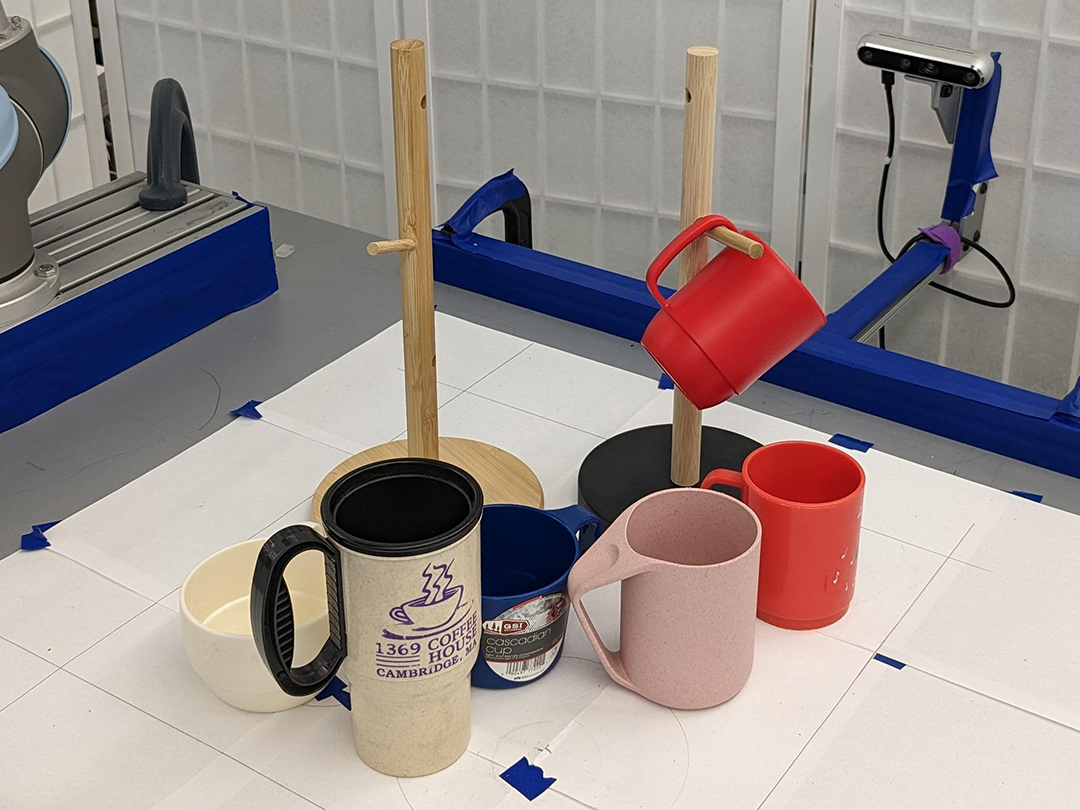
\includegraphics[width=\linewidth]{figures/object_sets/mug_on_tree.png}
        \caption{}
    \end{subfigure}
    \begin{subfigure}{(\linewidth - 0.05\linewidth)/3}
        \centering
        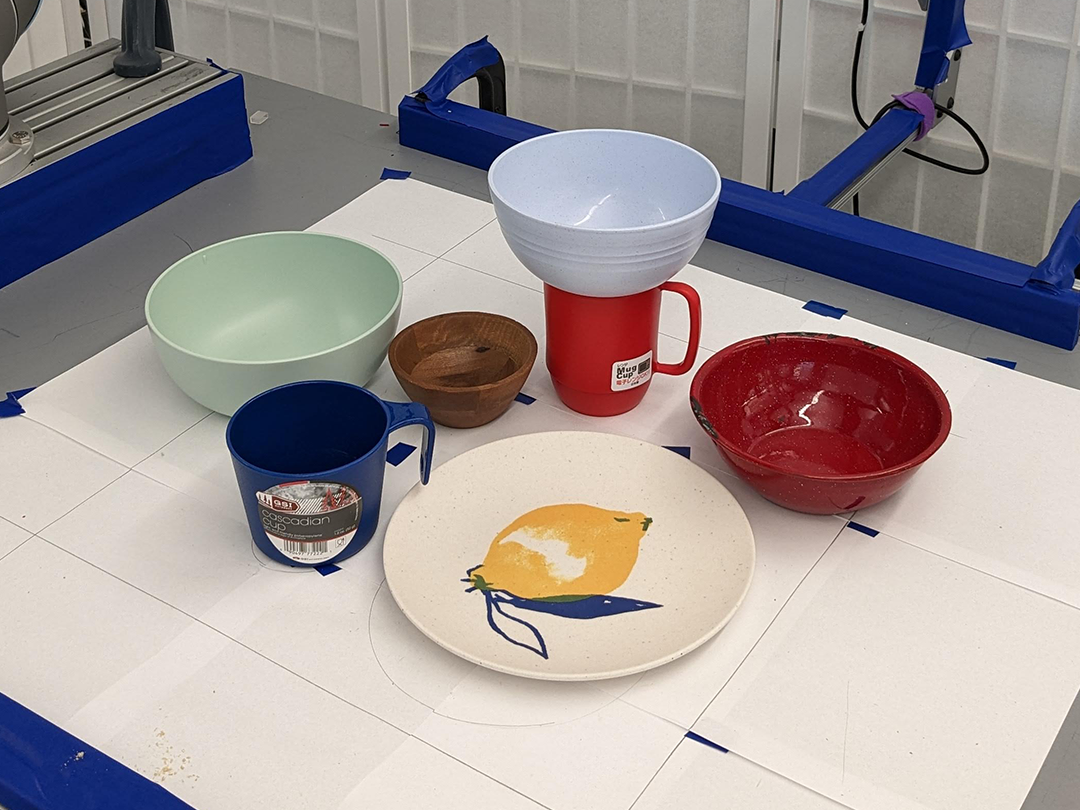
\includegraphics[width=\linewidth]{figures/object_sets/bowl_on_mug.png}
        \caption{}
    \end{subfigure}
    \begin{subfigure}{(\linewidth - 0.05\linewidth)/3}
        \centering
        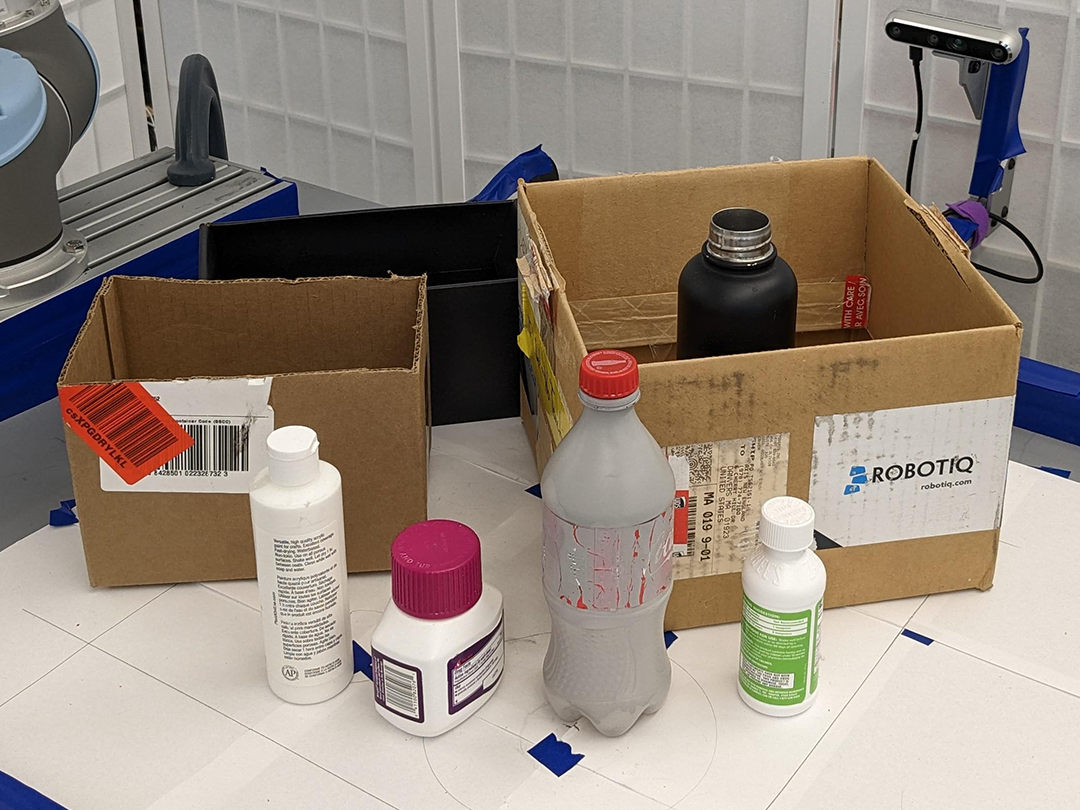
\includegraphics[width=\linewidth]{figures/object_sets/bottle_in_box.png}
        \caption{}
    \end{subfigure}

    \caption{Objects used for the real-world tasks: (a) mug on tree, (b) bowl (or plate) on mug and (c) bottle in box. We use a single pair of objects to generate demonstrations and test on novel objects.}
    \label{fig:object_sets}
\end{figure}

\subsection{Grasp prediction in the wild}
\label{appendix:experiment:wild}

We use a single RealSense D435 RGB-D camera. Our goal is to be able to demonstrate any task in the real world without having to re-train our perception pipeline. Therefore, we chose an open-vocabulary object detection model Detic \cite{zhou22detecting}, which is able to detect object based on natural language descriptions. We use the predicted bounding boxes from Detic to condition a Segment Anything model \cite{kirillov23segment} to get accurate class-agnostic segmentation masks. Both Detic\footnote{https://github.com/facebookresearch/Detic} and Segment Anything\footnote{https://github.com/facebookresearch/segment-anything} come with several pre-trained models and we used the largest available. Finally, we select the pixels within each segmentation mask and use the depth information from our depth camera to create a per-object point cloud. We use DBSCAN to clouster the point cloud and filter out outlier points. Then, we perform mesh warping and interaction warping to predict object meshes and grasps.

Previously, we experimented with Mask R-CNN \cite{he17mask} and Mask2Former \cite{cheng22maskedattention} trained on standard segmentation datasets, such as COCO \cite{lin15microsoft} and ADE20k \cite{scene}. We found that these dataset lack the wide range of object classes we would see in a household environment and that the trained models struggle with out-of-distribution viewing angles, such as looking from a steep top-down angle. We also experimented with an open-vocabulary object detection model OWL-ViT \cite{minderer22simple} and found it to be sensitive to scene clutter and the viewing angle.

% \ob{TODO: Re-write this to better fit into the paper.} In our project, our primary objective was to predict objects in the wild, so we chose DETIC, an object detection method capable of classifying 20,000+ classes. We concentrated on object detection and 3D semantic segmentation using PointNet. However, we encountered challenges with the PointNet network, which led us to adapt the experiment by performing 2D object detection, specifically for mugs or cups.
% We explored various methods for 2D object detection and semantic segmentation in different environments, including YOLO V8 Nano (Class Moderated), OWL ViT Image-Guided Detection, OWL ViT Text-Guided Detection, DETIC Object Detector, and the Segment Anything Model (SAM). Our focus was on the combination of SAM and DETIC, which we applied in home and lab environments to assess their performance and effectiveness.
% By employing DETIC for object detection with its vast range of classes, we aimed to improve the accuracy of the pipeline. We then used the output bounding boxes from DETIC as prompts for the SAM model, allowing us to achieve better segmentation results. This combination not only enhanced the overall accuracy and effectiveness of the pipeline but also highlighted the adaptability of the SAM model in various scenarios.
% Despite some limitations, our project provided valuable insights into the challenges of object detection and 3D semantic segmentation, emphasizing the importance of a more appropriate dataset and addressing the limitations of the PointNet network. Our efforts in combining DETIC and SAM demonstrated the potential of such an approach for future research in the field.
% \ob{Kishore -- RGBD to segmented point clouds to grasp candidates}

\section{Additional Experiments}

\begin{figure}[]
    \centering

    \begin{subfigure}{(\linewidth - 0.05\linewidth)/5}
        \centering
        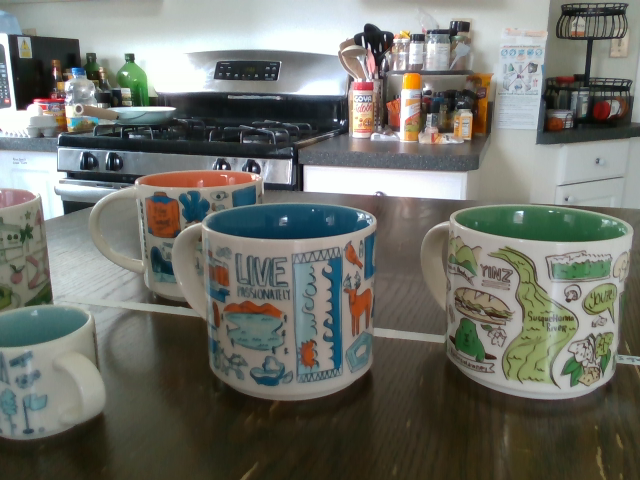
\includegraphics[width=\linewidth]{figures/real2sim2real/6/1.png}
    \end{subfigure}
    \begin{subfigure}{(\linewidth - 0.05\linewidth)/5}
        \centering
        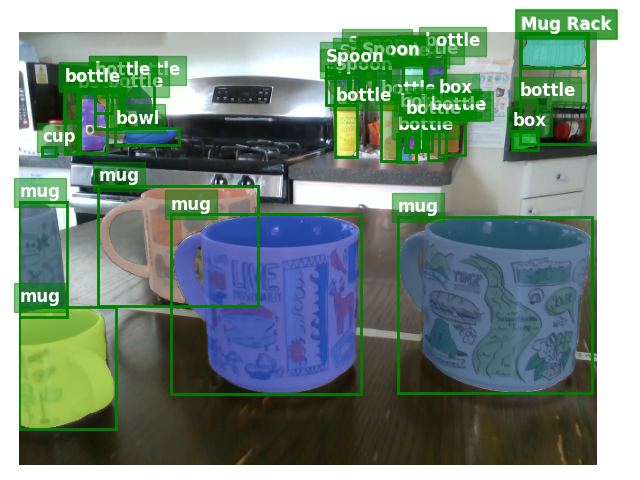
\includegraphics[width=\linewidth]{figures/real2sim2real/6/0.png}
    \end{subfigure}
    \begin{subfigure}{(\linewidth - 0.05\linewidth)/5}
        \centering
        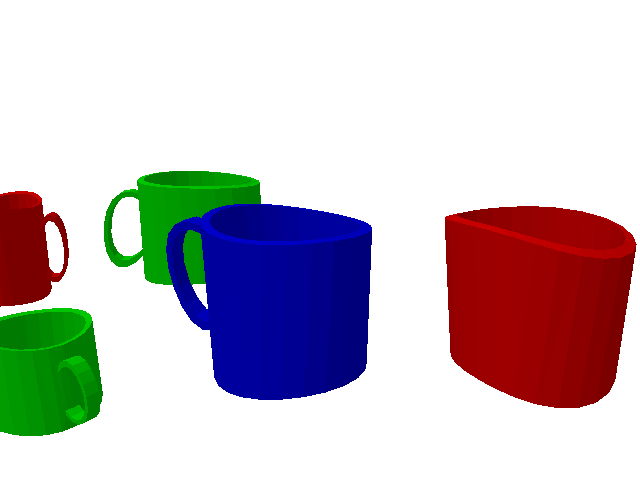
\includegraphics[width=\linewidth]{figures/real2sim2real/6/3_sim.png}
    \end{subfigure}
    \begin{subfigure}{(\linewidth - 0.05\linewidth)/5}
        \centering
        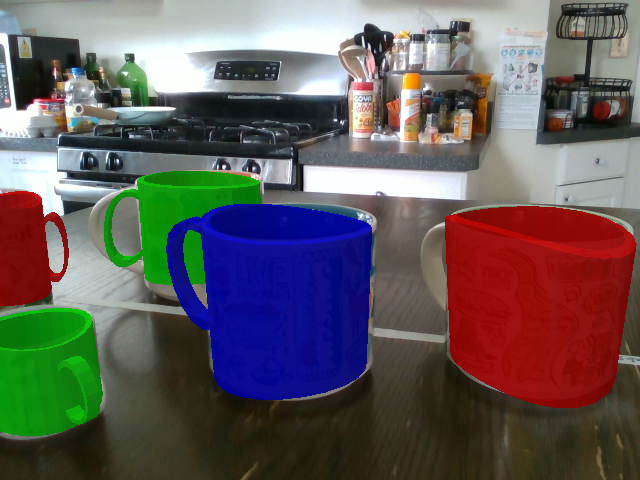
\includegraphics[width=\linewidth]{figures/real2sim2real/6/3.png}
    \end{subfigure}
    \begin{subfigure}{(\linewidth - 0.05\linewidth)/5}
        \centering
        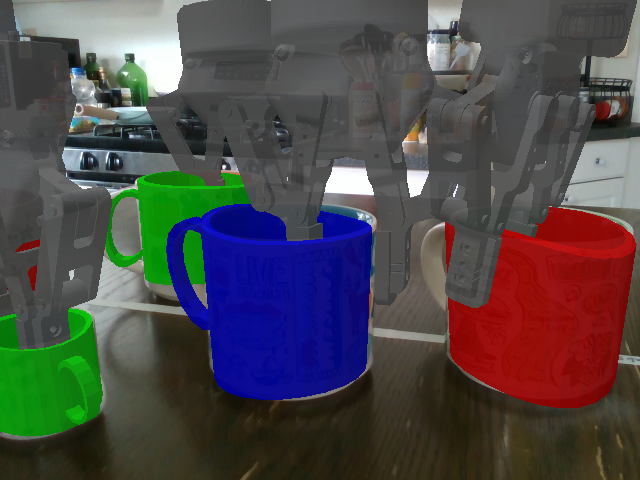
\includegraphics[width=\linewidth]{figures/real2sim2real/6/4.png}
    \end{subfigure}

    \begin{subfigure}{(\linewidth - 0.05\linewidth)/5}
        \centering
        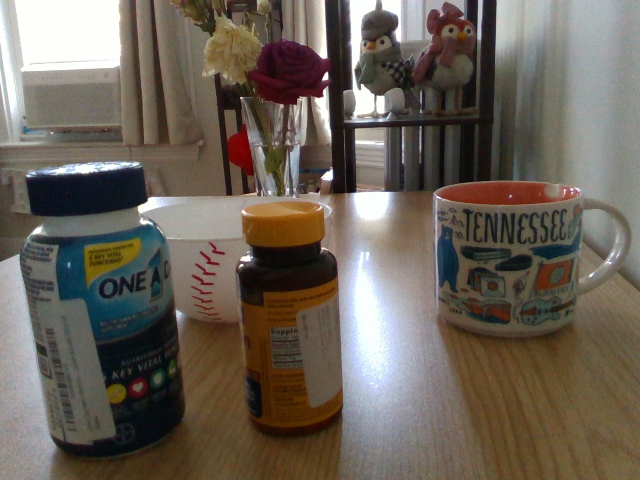
\includegraphics[width=\linewidth]{figures/real2sim2real/7/1.png}
    \end{subfigure}
    \begin{subfigure}{(\linewidth - 0.05\linewidth)/5}
        \centering
        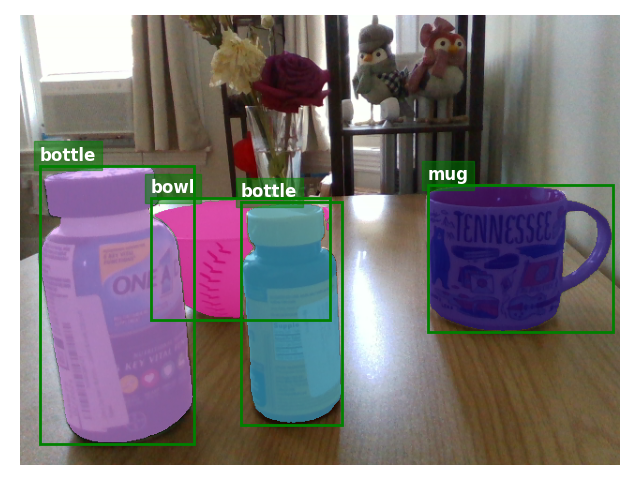
\includegraphics[width=\linewidth]{figures/real2sim2real/7/0.png}
    \end{subfigure}
    \begin{subfigure}{(\linewidth - 0.05\linewidth)/5}
        \centering
        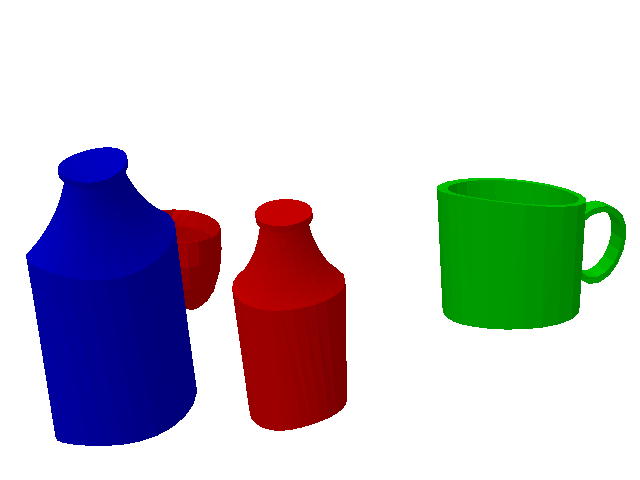
\includegraphics[width=\linewidth]{figures/real2sim2real/7/3_sim.png}
    \end{subfigure}
    \begin{subfigure}{(\linewidth - 0.05\linewidth)/5}
        \centering
        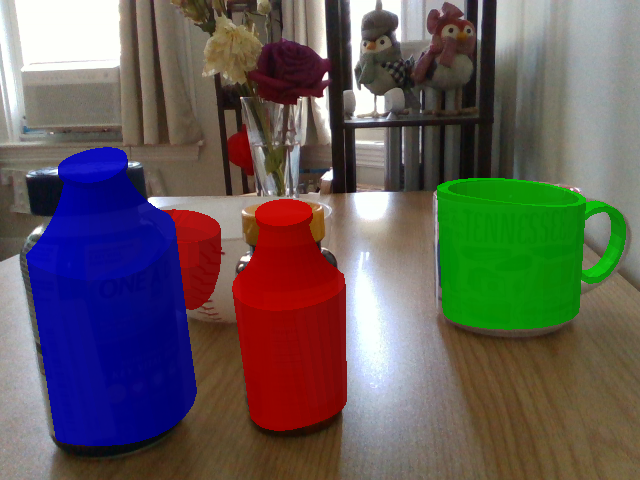
\includegraphics[width=\linewidth]{figures/real2sim2real/7/3.png}
    \end{subfigure}
    \begin{subfigure}{(\linewidth - 0.05\linewidth)/5}
        \centering
        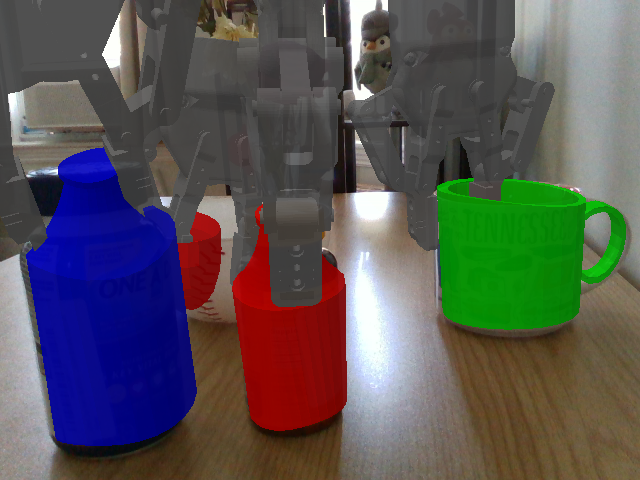
\includegraphics[width=\linewidth]{figures/real2sim2real/7/4.png}
    \end{subfigure}

    \begin{subfigure}{(\linewidth - 0.05\linewidth)/5}
        \centering
        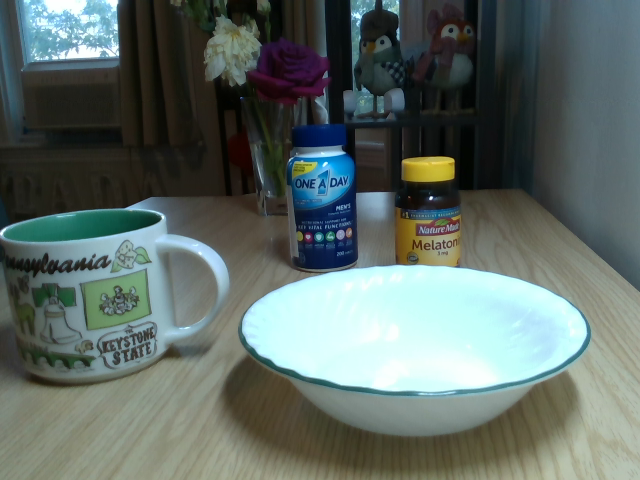
\includegraphics[width=\linewidth]{figures/real2sim2real/3/1.png}
    \end{subfigure}
    \begin{subfigure}{(\linewidth - 0.05\linewidth)/5}
        \centering
        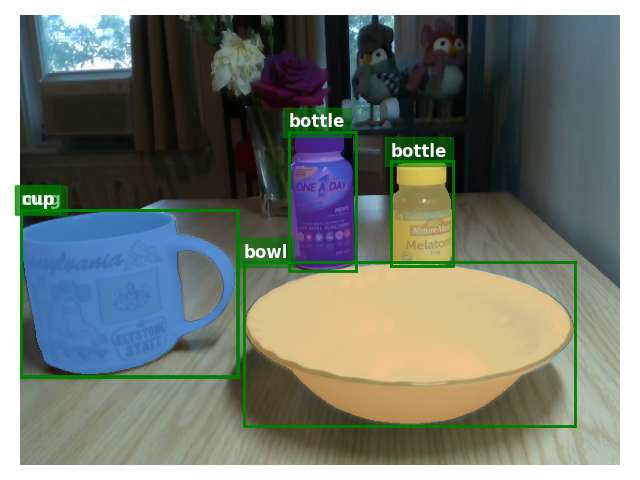
\includegraphics[width=\linewidth]{figures/real2sim2real/3/0.png}
    \end{subfigure}
    \begin{subfigure}{(\linewidth - 0.05\linewidth)/5}
        \centering
        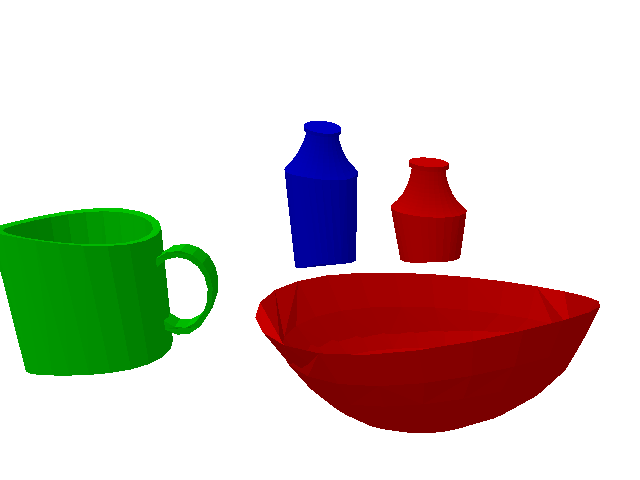
\includegraphics[width=\linewidth]{figures/real2sim2real/3/3_sim.png}
    \end{subfigure}
    \begin{subfigure}{(\linewidth - 0.05\linewidth)/5}
        \centering
        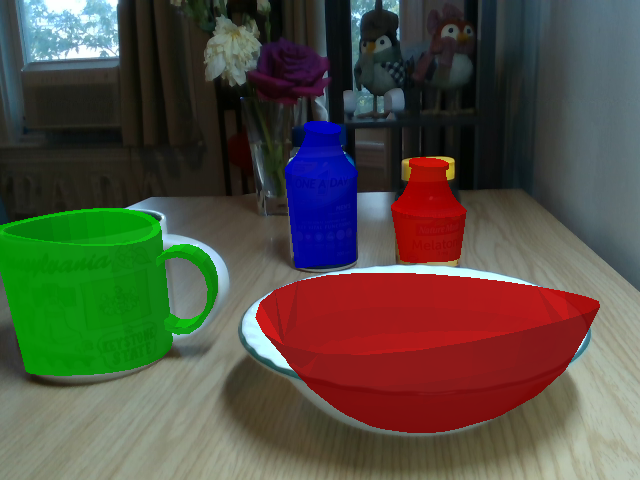
\includegraphics[width=\linewidth]{figures/real2sim2real/3/3.png}
    \end{subfigure}
    \begin{subfigure}{(\linewidth - 0.05\linewidth)/5}
        \centering
        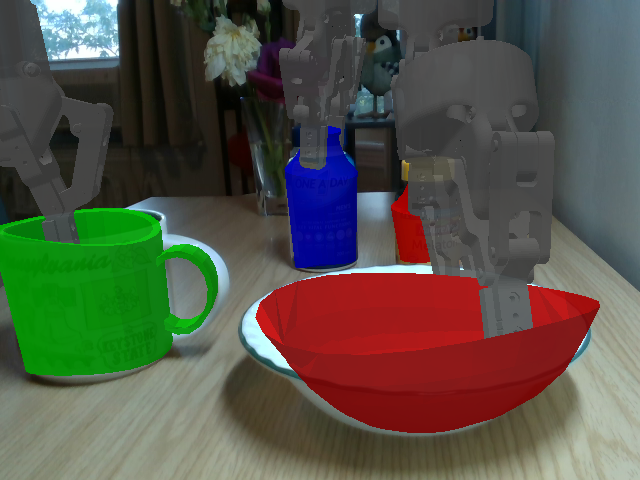
\includegraphics[width=\linewidth]{figures/real2sim2real/3/4.png}
    \end{subfigure}

    \begin{subfigure}{(\linewidth - 0.05\linewidth)/5}
        \centering
        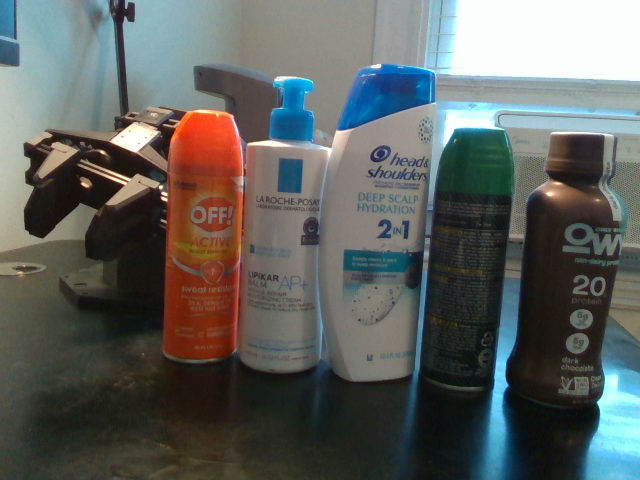
\includegraphics[width=\linewidth]{figures/real2sim2real/4/1.png}
    \end{subfigure}
    \begin{subfigure}{(\linewidth - 0.05\linewidth)/5}
        \centering
        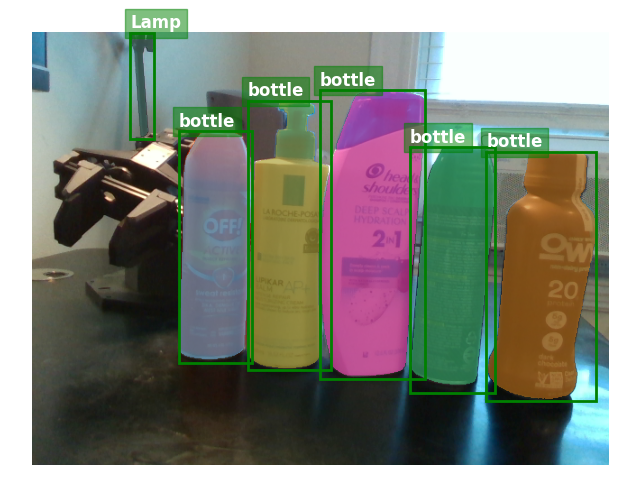
\includegraphics[width=\linewidth]{figures/real2sim2real/4/0.png}
    \end{subfigure}
    \begin{subfigure}{(\linewidth - 0.05\linewidth)/5}
        \centering
        \includegraphics[width=\linewidth]{figures/real2sim2real/4/3_sim.png}
    \end{subfigure}
    \begin{subfigure}{(\linewidth - 0.05\linewidth)/5}
        \centering
        \includegraphics[width=\linewidth]{figures/real2sim2real/4/3.png}
    \end{subfigure}
    \begin{subfigure}{(\linewidth - 0.05\linewidth)/5}
        \centering
        \includegraphics[width=\linewidth]{figures/real2sim2real/4/4.png}
    \end{subfigure}

    \begin{subfigure}{(\linewidth - 0.05\linewidth)/5}
        \centering
        \includegraphics[width=\linewidth]{figures/real2sim2real/8/1.png}
        \caption{}
    \end{subfigure}
    \begin{subfigure}{(\linewidth - 0.05\linewidth)/5}
        \centering
        \includegraphics[width=\linewidth]{figures/real2sim2real/8/0.png}
        \caption{}
    \end{subfigure}
    \begin{subfigure}{(\linewidth - 0.05\linewidth)/5}
        \centering
        \includegraphics[width=\linewidth]{figures/real2sim2real/8/3_sim.png}
        \caption{}
    \end{subfigure}
    \begin{subfigure}{(\linewidth - 0.05\linewidth)/5}
        \centering
        \includegraphics[width=\linewidth]{figures/real2sim2real/8/3.png}
        \caption{}
    \end{subfigure}
    \begin{subfigure}{(\linewidth - 0.05\linewidth)/5}
        \centering
        \includegraphics[width=\linewidth]{figures/real2sim2real/8/4.png}
        \caption{}
    \end{subfigure}

    \caption{Additional examples, please see Figure \ref{fig:real2sim2real}.}
    \label{fig:real2sim2real_part2}
\end{figure}

\end{document}
